\documentclass[twoside]{book}

% Packages required by doxygen
\usepackage{fixltx2e}
\usepackage{calc}
\usepackage{doxygen}
\usepackage[export]{adjustbox} % also loads graphicx
\usepackage{graphicx}
\usepackage[utf8]{inputenc}
\usepackage{makeidx}
\usepackage{multicol}
\usepackage{multirow}
\PassOptionsToPackage{warn}{textcomp}
\usepackage{textcomp}
\usepackage[nointegrals]{wasysym}
\usepackage[table]{xcolor}

% Font selection
\usepackage[T1]{fontenc}
\usepackage[scaled=.90]{helvet}
\usepackage{courier}
\usepackage{amssymb}
\usepackage{sectsty}
\renewcommand{\familydefault}{\sfdefault}
\allsectionsfont{%
  \fontseries{bc}\selectfont%
  \color{darkgray}%
}
\renewcommand{\DoxyLabelFont}{%
  \fontseries{bc}\selectfont%
  \color{darkgray}%
}
\newcommand{\+}{\discretionary{\mbox{\scriptsize$\hookleftarrow$}}{}{}}

% Page & text layout
\usepackage{geometry}
\geometry{%
  a4paper,%
  top=2.5cm,%
  bottom=2.5cm,%
  left=2.5cm,%
  right=2.5cm%
}
\tolerance=750
\hfuzz=15pt
\hbadness=750
\setlength{\emergencystretch}{15pt}
\setlength{\parindent}{0cm}
\setlength{\parskip}{3ex plus 2ex minus 2ex}
\makeatletter
\renewcommand{\paragraph}{%
  \@startsection{paragraph}{4}{0ex}{-1.0ex}{1.0ex}{%
    \normalfont\normalsize\bfseries\SS@parafont%
  }%
}
\renewcommand{\subparagraph}{%
  \@startsection{subparagraph}{5}{0ex}{-1.0ex}{1.0ex}{%
    \normalfont\normalsize\bfseries\SS@subparafont%
  }%
}
\makeatother

% Headers & footers
\usepackage{fancyhdr}
\pagestyle{fancyplain}
\fancyhead[LE]{\fancyplain{}{\bfseries\thepage}}
\fancyhead[CE]{\fancyplain{}{}}
\fancyhead[RE]{\fancyplain{}{\bfseries\leftmark}}
\fancyhead[LO]{\fancyplain{}{\bfseries\rightmark}}
\fancyhead[CO]{\fancyplain{}{}}
\fancyhead[RO]{\fancyplain{}{\bfseries\thepage}}
\fancyfoot[LE]{\fancyplain{}{}}
\fancyfoot[CE]{\fancyplain{}{}}
\fancyfoot[RE]{\fancyplain{}{\bfseries\scriptsize Generated by Doxygen }}
\fancyfoot[LO]{\fancyplain{}{\bfseries\scriptsize Generated by Doxygen }}
\fancyfoot[CO]{\fancyplain{}{}}
\fancyfoot[RO]{\fancyplain{}{}}
\renewcommand{\footrulewidth}{0.4pt}
\renewcommand{\chaptermark}[1]{%
  \markboth{#1}{}%
}
\renewcommand{\sectionmark}[1]{%
  \markright{\thesection\ #1}%
}

% Indices & bibliography
\usepackage{natbib}
\usepackage[titles]{tocloft}
\setcounter{tocdepth}{3}
\setcounter{secnumdepth}{5}
\makeindex

% Hyperlinks (required, but should be loaded last)
\usepackage{ifpdf}
\ifpdf
  \usepackage[pdftex,pagebackref=true]{hyperref}
\else
  \usepackage[ps2pdf,pagebackref=true]{hyperref}
\fi
\hypersetup{%
  colorlinks=true,%
  linkcolor=blue,%
  citecolor=blue,%
  unicode%
}

% Custom commands
\newcommand{\clearemptydoublepage}{%
  \newpage{\pagestyle{empty}\cleardoublepage}%
}

\usepackage{caption}
\captionsetup{labelsep=space,justification=centering,font={bf},singlelinecheck=off,skip=4pt,position=top}

%===== C O N T E N T S =====

\begin{document}

% Titlepage & ToC
\hypersetup{pageanchor=false,
             bookmarksnumbered=true,
             pdfencoding=unicode
            }
\pagenumbering{alph}
\begin{titlepage}
\vspace*{7cm}
\begin{center}%
{\Large generate\+\_\+packings \\[1ex]\large 1.\+0.\+0 }\\
\vspace*{1cm}
{\large Generated by Doxygen 1.8.14}\\
\end{center}
\end{titlepage}
\clearemptydoublepage
\pagenumbering{roman}
\tableofcontents
\clearemptydoublepage
\pagenumbering{arabic}
\hypersetup{pageanchor=true}

%--- Begin generated contents ---
\chapter{Quickstart Guide}
\label{index}\hypertarget{index}{}\hypertarget{index_getting_code}{}\section{Getting the code}\label{index_getting_code}
Getting started with generate\+\_\+packings is easy. Make sure you have a system capable of compiling C++ (g++ or clang) and obtain the repo via\+: 
\begin{DoxyCode}
$ git clone https:\textcolor{comment}{//github.com/jacktreado/generate\_packings}
$ cd generate\_packings
\end{DoxyCode}
 Once you have a local copy, to test it do the following\+:


\begin{DoxyCode}
$ cd examples/test\_main\_files
$ g++ -I ../../src/ residue\_pack\_test.cpp ../../src/\mbox{\hyperlink{classrigidbody}{rigidbody}}.cpp ../../src/
      \mbox{\hyperlink{classpacking}{packing}}*.cpp ../../src/\mbox{\hyperlink{class_quaternion}{Quaternion}}.cpp -o test.o
$ ./test.o
\end{DoxyCode}


Once the simulation is complete, you should see something like this, indicative of success\+:


\begin{DoxyCode}
Contact Matrix:
     0     0     0     1     1     1     1     0     1     0     0     1
     0     0     0     1     0     0     1     1     0     1     1     0
     0     0     0     0     1     0     1     0     0     1     1     1
     1     1     0     0     0     1     0     0     1     1     1     0
     1     0     1     0     0     1     0     1     0     0     1     1
     1     0     0     1     1     0     1     1     1     0     0     0
     1     1     1     0     0     1     0     0     1     1     0     1
     0     1     0     0     1     1     0     0     1     1     1     1
     1     0     0     1     0     1     1     1     0     0     1     1
     0     1     1     1     0     0     1     1     0     0     1     0
     0     1     1     1     1     0     0     1     1     1     0     1
     1     0     1     0     1     0     1     1     1     0     1     0


~entering \mbox{\hyperlink{classrigidbody}{rigidbody}} destructor
\end{DoxyCode}
\hypertarget{index_writing_sims}{}\section{Running your own simulations}\label{index_writing_sims}
If you open up {\ttfamily residue\+\_\+pack\+\_\+test.\+cpp} you can take a look at some key areas of the code that should be modified if you are to run your own simulation.

Along with all the other imports at the top of the file, be sure to include {\ttfamily \mbox{\hyperlink{rigidbody_8h}{rigidbody.\+h}}}


\begin{DoxyCode}
\textcolor{preprocessor}{#include "\mbox{\hyperlink{rigidbody_8h}{rigidbody.h}}"}
\textcolor{preprocessor}{#include <iostream>}
\textcolor{preprocessor}{#include <fstream>}
\textcolor{preprocessor}{#include <string>}
\textcolor{preprocessor}{#include <cstdlib>}
\end{DoxyCode}
 
\chapter{Hierarchical Index}
\section{Class Hierarchy}
This inheritance list is sorted roughly, but not completely, alphabetically\+:\begin{DoxyCompactList}
\item \contentsline{section}{packing}{\pageref{classpacking}}{}
\begin{DoxyCompactList}
\item \contentsline{section}{rigidbody}{\pageref{classrigidbody}}{}
\end{DoxyCompactList}
\item \contentsline{section}{Quaternion}{\pageref{class_quaternion}}{}
\end{DoxyCompactList}

\chapter{Class Index}
\section{Class List}
Here are the classes, structs, unions and interfaces with brief descriptions\+:\begin{DoxyCompactList}
\item\contentsline{section}{\mbox{\hyperlink{classpacking}{packing}} }{\pageref{classpacking}}{}
\item\contentsline{section}{\mbox{\hyperlink{class_quaternion}{Quaternion}} }{\pageref{class_quaternion}}{}
\item\contentsline{section}{\mbox{\hyperlink{classrigidbody}{rigidbody}} }{\pageref{classrigidbody}}{}
\end{DoxyCompactList}

\chapter{File Index}
\section{File List}
Here is a list of all files with brief descriptions\+:\begin{DoxyCompactList}
\item\contentsline{section}{src/\mbox{\hyperlink{packing_8cpp}{packing.\+cpp}} }{\pageref{packing_8cpp}}{}
\item\contentsline{section}{src/\mbox{\hyperlink{packing_8h}{packing.\+h}} }{\pageref{packing_8h}}{}
\item\contentsline{section}{src/\mbox{\hyperlink{packing__meas_8cpp}{packing\+\_\+meas.\+cpp}} }{\pageref{packing__meas_8cpp}}{}
\item\contentsline{section}{src/\mbox{\hyperlink{packing__sim_8cpp}{packing\+\_\+sim.\+cpp}} }{\pageref{packing__sim_8cpp}}{}
\item\contentsline{section}{src/\mbox{\hyperlink{packing__test_8cpp}{packing\+\_\+test.\+cpp}} }{\pageref{packing__test_8cpp}}{}
\item\contentsline{section}{src/\mbox{\hyperlink{_quaternion_8cpp}{Quaternion.\+cpp}} }{\pageref{_quaternion_8cpp}}{}
\item\contentsline{section}{src/\mbox{\hyperlink{_quaternion_8h}{Quaternion.\+h}} }{\pageref{_quaternion_8h}}{}
\item\contentsline{section}{src/\mbox{\hyperlink{rigidbody_8cpp}{rigidbody.\+cpp}} }{\pageref{rigidbody_8cpp}}{}
\item\contentsline{section}{src/\mbox{\hyperlink{rigidbody_8h}{rigidbody.\+h}} }{\pageref{rigidbody_8h}}{}
\end{DoxyCompactList}

\chapter{Class Documentation}
\hypertarget{classpacking}{}\section{packing Class Reference}
\label{classpacking}\index{packing@{packing}}


This is the packing base class. The rigidbody class inherits from it.  




{\ttfamily \#include $<$packing.\+h$>$}

Inheritance diagram for packing\+:\begin{figure}[H]
\begin{center}
\leavevmode
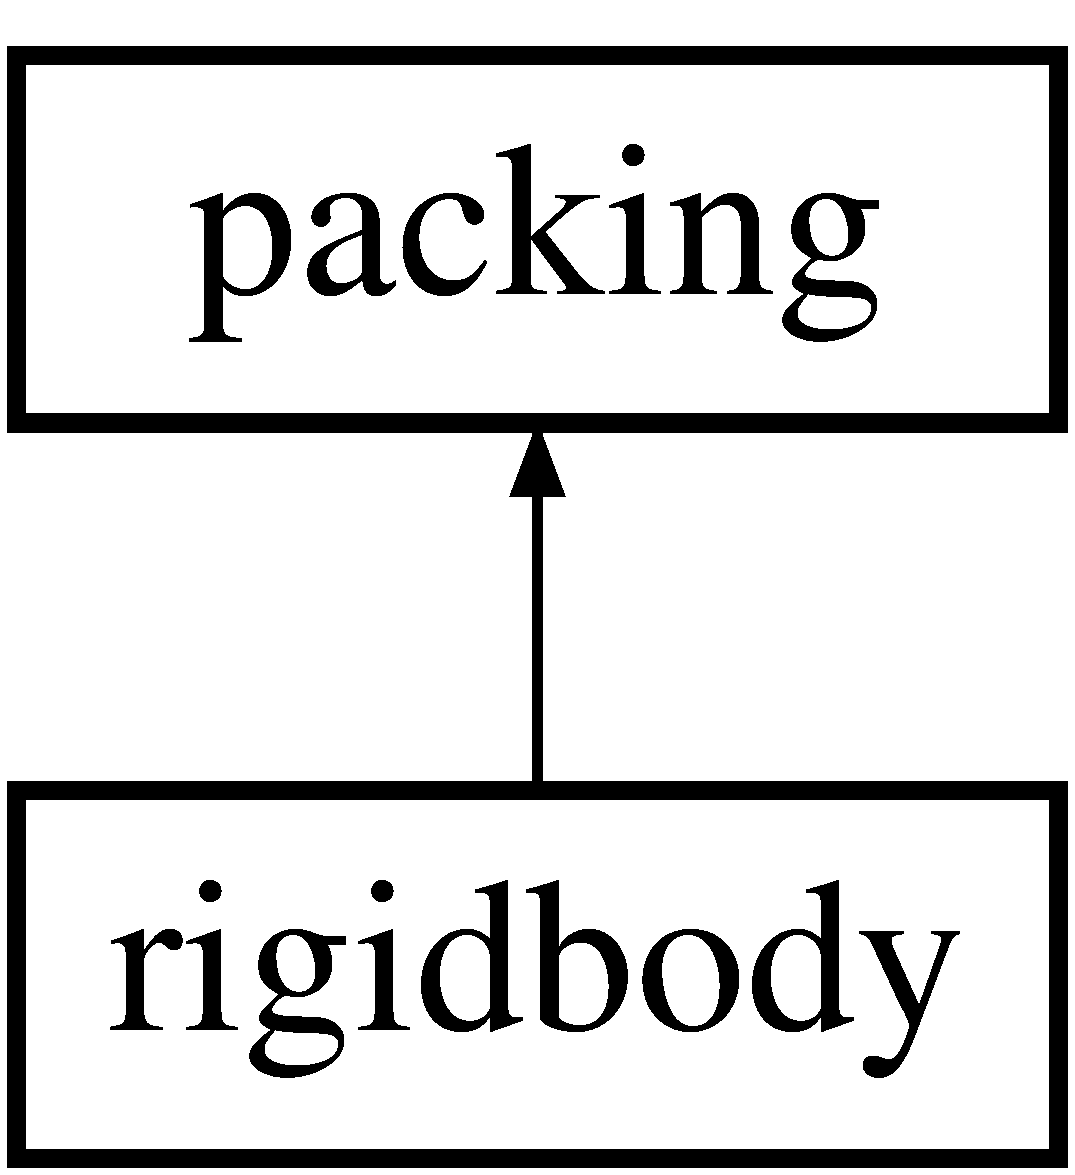
\includegraphics[height=2.000000cm]{classpacking}
\end{center}
\end{figure}
\subsection*{Public Member Functions}
\begin{DoxyCompactItemize}
\item 
\mbox{\hyperlink{classpacking_aec1b63190de5c8e69e47a06bfb7db0d5}{packing}} (int n, int dof, int nc, int s)
\item 
\mbox{\hyperlink{classpacking_ac345d2c7345a103d7b390585565d2712}{packing}} (std\+::string \&str, int ndim, int s)
\item 
\mbox{\hyperlink{classpacking_a954ef88de3bcf03906e7b9c1511c4338}{packing}} (int n, int ndim, double \mbox{\hyperlink{classpacking_a9683c4c16704f81b0086a7639f030953}{alpha}}, double phi0, int \mbox{\hyperlink{classpacking_aa5a588c50b2c22b3c2917a2da12f33e5}{seed}})
\item 
\mbox{\hyperlink{classpacking_ae34dd16515628814825132a9dbf06543}{packing}} (int n, int ndim, double \mbox{\hyperlink{classpacking_a9683c4c16704f81b0086a7639f030953}{alpha}}, double phi0, int nc, int nnu, double rc, int \mbox{\hyperlink{classpacking_aa5a588c50b2c22b3c2917a2da12f33e5}{seed}})
\item 
\mbox{\hyperlink{classpacking_a985cd1712c1e0c7e9f3927e847383810}{$\sim$packing}} ()
\item 
void \mbox{\hyperlink{classpacking_a00d1be8bf289c4a8a29fa915c9db13e9}{initialize\+\_\+\+NC}} ()
\item 
void \mbox{\hyperlink{classpacking_a16af9b32d0aa64fe236bc73ca5b98248}{initialize\+\_\+box}} (double val)
\item 
void \mbox{\hyperlink{classpacking_a87d6f5a31dd8c3c0f30c40f6e8b478f2}{initialize\+\_\+particles}} ()
\item 
void \mbox{\hyperlink{classpacking_af1514931993a8ea4fd14ff53f7d38b70}{initialize\+\_\+nlcl}} ()
\item 
void \mbox{\hyperlink{classpacking_a1f49ca3dbade782f8da82c946a2be238}{setup\+\_\+nlcl}} ()
\item 
void \mbox{\hyperlink{classpacking_aff094d1084949ed63ca374373e8d312b}{freeze\+\_\+nlcl}} ()
\item 
void \mbox{\hyperlink{classpacking_a02683527b4a5e41e2b9eaac44672cf9f}{setup\+\_\+std\+\_\+\+F\+I\+RE}} ()
\item 
void \mbox{\hyperlink{classpacking_afc22f53f3fa942d5347a3ebfeacae2bf}{setup\+\_\+std\+\_\+sim}} ()
\item 
void \mbox{\hyperlink{classpacking_a706d5c77cb054dadbf181fe1b68c6eda}{mc\+\_\+pos\+\_\+init}} ()
\item 
void \mbox{\hyperlink{classpacking_ad096a61ae3cd07d3a85f0c865ec0af70}{mxwl\+\_\+vel\+\_\+init}} (double t)
\item 
void \mbox{\hyperlink{classpacking_afa5fb6a5af7e185656c85f10534572a9}{rand\+\_\+vel\+\_\+init}} (double tmp0)
\item 
void \mbox{\hyperlink{classpacking_a15619b62e055ec5e1897fb8d40b194b2}{read\+\_\+spheres}} (std\+::string \&str)
\item 
int \mbox{\hyperlink{classpacking_addc33dab6e59ce3a959b1987ac0a4fce}{get\+\_\+N}} ()
\item 
int \mbox{\hyperlink{classpacking_a09b1231993da19d68581f630365d0c3a}{get\+\_\+\+N\+D\+IM}} ()
\item 
int \mbox{\hyperlink{classpacking_a0b60c2368d6b16389edfdb81bd0f45b7}{get\+\_\+\+D\+OF}} ()
\item 
int \mbox{\hyperlink{classpacking_ac99ab03b903298da3ac29dde9fdd4ad1}{get\+\_\+seed}} ()
\item 
double \mbox{\hyperlink{classpacking_a778812fa17eb4daa96adc03f1ce5128c}{get\+\_\+dt}} ()
\item 
double \mbox{\hyperlink{classpacking_a08f9bf70b057ad530e1499c15fdb34ff}{get\+\_\+phi}} ()
\item 
double \mbox{\hyperlink{classpacking_abe5e5105ed2b581e64f0ba5608e2ccb6}{get\+\_\+ep}} ()
\item 
double \mbox{\hyperlink{classpacking_ac2544dd44e1dd8bfb08315f94d543bc3}{get\+\_\+U}} ()
\item 
double \mbox{\hyperlink{classpacking_ab484a3d36c45db72614267af5a203f76}{get\+\_\+K}} ()
\item 
double \mbox{\hyperlink{classpacking_a366b4efa1f1fecf098df6bb9af09e739}{get\+\_\+alpha}} ()
\item 
double \mbox{\hyperlink{classpacking_a357aeeeac709d7926cbbaa9312cf3649}{get\+\_\+alpha0}} ()
\item 
double \mbox{\hyperlink{classpacking_a58b555de4a9902399b3ab82dabfefd12}{get\+\_\+finc}} ()
\item 
double \mbox{\hyperlink{classpacking_a2b4e47ab0671d9ee9892495df465be17}{get\+\_\+fdec}} ()
\item 
double \mbox{\hyperlink{classpacking_a0c8cad7afd9da1c30856b1201be15535}{get\+\_\+falpha}} ()
\item 
double \mbox{\hyperlink{classpacking_a36de243c3a970bbf0840a17bf9758e61}{get\+\_\+dtmax}} ()
\item 
double \mbox{\hyperlink{classpacking_acf25ed42e0fdfc8334d9c6468e5c34e1}{get\+\_\+distance}} (int p1, int p2)
\item 
double \mbox{\hyperlink{classpacking_a79d854d4f45683e8a11652ce90676a90}{get\+\_\+distance}} (int p1, int p2, double xij\mbox{[}$\,$\mbox{]})
\item 
double \mbox{\hyperlink{classpacking_a9485b9495dbedd5d954bade26a3033b7}{get\+\_\+rcut}} ()
\item 
double \mbox{\hyperlink{classpacking_a72af770ca74d1b7cf93301210b4aee63}{get\+\_\+mean\+\_\+vel}} ()
\item 
double \mbox{\hyperlink{classpacking_a654616abad6b4e39903bf1c2f4953c8a}{get\+\_\+com}} ()
\item 
double \mbox{\hyperlink{classpacking_aed06b7bd33506e2e26fd4b95749873a8}{get\+\_\+mean\+\_\+mass}} ()
\item 
double \mbox{\hyperlink{classpacking_ace5de1e50143754b63f3922ed9dcd646}{get\+\_\+mean\+\_\+rad}} ()
\item 
double \mbox{\hyperlink{classpacking_a23fc5018721f5022318addbe87b33d47}{get\+\_\+c\+\_\+sum}} ()
\item 
void \mbox{\hyperlink{classpacking_aa6f391cfee43bbb59dc71221a23c8d83}{reset\+\_\+c}} ()
\item 
void \mbox{\hyperlink{classpacking_a33a628e0d2d7bcaa72f6a205a3244e76}{set\+\_\+alpha0}} (double val)
\item 
void \mbox{\hyperlink{classpacking_aa80ff9c4b9ec36807a0d42ce28f50d2a}{set\+\_\+alpha}} (double val)
\item 
void \mbox{\hyperlink{classpacking_a8cb03b2d0af8408ba4c590ade7c738ca}{set\+\_\+finc}} (double val)
\item 
void \mbox{\hyperlink{classpacking_aaa7a1eb80bdf6f80a8d91415e4e03e69}{set\+\_\+fdec}} (double val)
\item 
void \mbox{\hyperlink{classpacking_af80acfd978be8d09fed22d40459bb3fc}{set\+\_\+falpha}} (double val)
\item 
void \mbox{\hyperlink{classpacking_a5dc1a61832b80ca41be310784cec6008}{set\+\_\+dtmax}} (double val)
\item 
void \mbox{\hyperlink{classpacking_a9c34cb0d24ff7bf013c19f801591c646}{set\+\_\+plotskip}} (int val)
\item 
void \mbox{\hyperlink{classpacking_a9bfa5637ac07f61d5cd34655c3a36455}{set\+\_\+plotit}} (int val)
\item 
void \mbox{\hyperlink{classpacking_a2d86b4b1188bd7d3c9b13dacbb0ca2fb}{set\+\_\+dt}} (double val)
\item 
void \mbox{\hyperlink{classpacking_a3371ec250e3165eae9231914a7e7fa88}{set\+\_\+ep}} (double val)
\item 
void \mbox{\hyperlink{classpacking_a073820579ccf298710943fefe023d853}{set\+\_\+rcut}} (double val)
\item 
void \mbox{\hyperlink{classpacking_af02fd953055fe009e6d3e79cc7a22eb8}{set\+\_\+phi}} (double val)
\item 
void \mbox{\hyperlink{classpacking_aab96c0f738b9ff52cf5eb9deba301387}{set\+\_\+md\+\_\+time}} (double dt0)
\item 
void \mbox{\hyperlink{classpacking_ab1b640756b858f5df25d88ab841300b2}{set\+\_\+rand\+\_\+c}} (double p)
\item 
void \mbox{\hyperlink{classpacking_a7d0e7e1a244a3cb1080a5b8c189a3373}{update\+\_\+cell\+\_\+g}} ()
\item 
void \mbox{\hyperlink{classpacking_a0c837c1a1a49e78d98e3caa99452ba48}{open\+\_\+xyz}} (std\+::string str)
\item 
void \mbox{\hyperlink{classpacking_a0c981ac48ac009de032b346acd442527}{open\+\_\+config}} (std\+::string str)
\item 
void \mbox{\hyperlink{classpacking_aafe0cb05420e66caa923930222ff1bb0}{open\+\_\+stat}} (std\+::string str)
\item 
void \mbox{\hyperlink{classpacking_a8afd538218a84fa24e14d58ecbd8066b}{open\+\_\+en}} (std\+::string str)
\item 
void \mbox{\hyperlink{classpacking_a0674ff540e56b7de2919fea2960b7703}{pos\+\_\+update}} ()
\item 
double \mbox{\hyperlink{classpacking_a87346c3bda1750e3a75fcb626ccaf82f}{hs}} (double sij, double xij)
\item 
void \mbox{\hyperlink{classpacking_a2506d13784217eda51bcb99b6005c94d}{hs\+\_\+force}} ()
\item 
void \mbox{\hyperlink{classpacking_aee29c91dd4747aca62cfecfb5197f87a}{hs\+\_\+force\+\_\+nn}} ()
\item 
void \mbox{\hyperlink{classpacking_a027c3c89940dc7e8b317368ed32cfc15}{vel\+\_\+update}} ()
\item 
int \mbox{\hyperlink{classpacking_a6c94dc46459e4acd96bc99d43ed257b2}{rmv\+\_\+rattlers}} (int \&krcrs)
\item 
void \mbox{\hyperlink{classpacking_ac31d7a9a0e3fde8ca3b527f6fc3f2b45}{catch\+\_\+nans}} (int t)
\item 
void \mbox{\hyperlink{classpacking_a4a4cc64305d5f1726e1a49e5a395f7e9}{md\+\_\+evol\+\_\+hs}} (double tmp0, int NT)
\item 
void \mbox{\hyperlink{classpacking_aa78e20cbe7bb48eb52a319a7eaac0b92}{jamming\+\_\+finder}} (double tend, double dphi, double Utol, double Ktol)
\item 
void \mbox{\hyperlink{classpacking_a09872b70b71323f159a3490073aa1741}{jamming\+\_\+finder\+\_\+nn}} (double tend, double dphi, double Utol, double Ktol)
\item 
void \mbox{\hyperlink{classpacking_af0edc401a0cb530600f0219e24518f23}{fire}} ()
\item 
void \mbox{\hyperlink{classpacking_a7560d84cdb496db31c6314c3a82b10e0}{root\+\_\+search}} (double \&phiH, double \&phiL, int \&check\+\_\+ratterls, int epconst, int \mbox{\hyperlink{classpacking_a31eede3d604c45fef6021170ee506c77}{nr}}, double dphi0, double Ktol, double Utol, int t)
\item 
void \mbox{\hyperlink{classpacking_af52187be2ba3d6cc25189c7cd389ba18}{print\+\_\+cell}} ()
\item 
void \mbox{\hyperlink{classpacking_aec21a0ddfaaa3153f016ee91901b0197}{print\+\_\+neighborlist}} ()
\item 
void \mbox{\hyperlink{classpacking_a6f594a2ebfaaf03a8a43f31d5e170b86}{print\+\_\+cell\+\_\+neighbors}} ()
\item 
void \mbox{\hyperlink{classpacking_a2b2c2908beb3d2577c01d4db73e7e2c1}{print\+\_\+nl\+\_\+xyz}} ()
\item 
void \mbox{\hyperlink{classpacking_a1dfafb1273eef9839012796f8f674cd3}{print\+\_\+cell\+\_\+pos}} ()
\item 
void \mbox{\hyperlink{classpacking_ac064578aca74b4916463599a9fbdf2af}{print\+\_\+clabel}} ()
\item 
void \mbox{\hyperlink{classpacking_a874b2bf73b23b4e051c293f68e25e6c9}{print\+\_\+celln}} ()
\item 
void \mbox{\hyperlink{classpacking_a433ee4f918ce8124cc4dc24a29dcbe1c}{add\+\_\+cell}} (int \mbox{\hyperlink{classpacking_ab06bef3feef42f5c48c39fa1ae297e23}{m}}, int i)
\item 
void \mbox{\hyperlink{classpacking_a7f866169806cadb74aaed38e246d11e5}{reset\+\_\+cells}} ()
\item 
void \mbox{\hyperlink{classpacking_a9a47d7d55eb9fa7a4083571fc2a9b78f}{add\+\_\+neighbor}} (int i, int j)
\item 
void \mbox{\hyperlink{classpacking_a9c073e15bbafc308692fb63f6390a843}{reset\+\_\+neighborlist}} (int i)
\item 
void \mbox{\hyperlink{classpacking_ac55b5f684a8767d536c671f23eea808e}{update\+\_\+celln}} ()
\item 
void \mbox{\hyperlink{classpacking_a51875315e1e8c16a5dfc9e3807fcff17}{get\+\_\+cell\+\_\+neighbors}} ()
\item 
void \mbox{\hyperlink{classpacking_ad9908dd91b3969dc8a5de39d8fcf66e3}{get\+\_\+cell\+\_\+positions}} ()
\item 
int \mbox{\hyperlink{classpacking_ac1311816bef393e5fccbbf61acefcb89}{get\+\_\+new\+\_\+cell}} (int i)
\item 
void \mbox{\hyperlink{classpacking_a944bd29a56c2811a991174ddb18aba63}{update\+\_\+cell}} ()
\item 
void \mbox{\hyperlink{classpacking_adf9ce1e5fca0258a3c93cd76652ecc50}{update\+\_\+neighborlist}} ()
\item 
void \mbox{\hyperlink{classpacking_a16f87413335e58b0ac9a9ded8742f32b}{scale\+\_\+sys}} (double dphi)
\item 
void \mbox{\hyperlink{classpacking_afaa70769d1b1faadad9e530f09fe26b9}{calc\+\_\+vacf}} (int NT, int vsave, std\+::ofstream \&obj)
\item 
void \mbox{\hyperlink{classpacking_ab91f79587ed1579f6754e956e7939597}{get\+\_\+vacf}} (int t, int vsave, std\+::vector$<$ double $>$ $\ast$$\ast$vlist, std\+::vector$<$ double $>$ \&numer, std\+::vector$<$ double $>$ \&denom)
\item 
void \mbox{\hyperlink{classpacking_a4eaacbf9a4212c3bdf61315317b21529}{finish\+\_\+vacf}} (int NT, int vsave, std\+::vector$<$ double $>$ \&numer, std\+::vector$<$ double $>$ \&denom, std\+::vector$<$ double $>$ \&vacf)
\item 
void \mbox{\hyperlink{classpacking_a50f911bdce5d1a3c81bd73eb3a77fd0e}{print\+\_\+vacf}} (int NT, int vsave, std\+::vector$<$ double $>$ \&vacf, std\+::ofstream \&obj)
\item 
void \mbox{\hyperlink{classpacking_ad87b894a228262a83190cae54f8a8bb2}{calc\+\_\+dm}} (std\+::string \&fstr)
\item 
double \mbox{\hyperlink{classpacking_a9e94b699c2cc7d52a74cd2e4a8642371}{perturb\+\_\+single\+\_\+particle}} (int i, int k, double h)
\item 
double \mbox{\hyperlink{classpacking_aa9d162db11496df9f1dd4696fe1924da}{perturb\+\_\+two\+\_\+particles}} (int i, int j, int k, int l, double h)
\item 
void \mbox{\hyperlink{classpacking_af2e5ff650c513fb8f69e0c1dd97a7ec7}{md\+\_\+monitor}} (int t, int \mbox{\hyperlink{classpacking_a31eede3d604c45fef6021170ee506c77}{nr}}, double phiH, double phiL)
\item 
void \mbox{\hyperlink{classpacking_a810b179015e89063c7af6e5e3588380c}{print\+\_\+xyz}} ()
\item 
void \mbox{\hyperlink{classpacking_ad65b44ad181d5311b6f4b2177b118f82}{print\+\_\+c\+\_\+mat}} ()
\item 
void \mbox{\hyperlink{classpacking_ab6181af7330866576f5f6e5ad42446a3}{print\+\_\+c\+\_\+mat}} (std\+::ofstream \&obj)
\item 
void \mbox{\hyperlink{classpacking_a4d5591724c0cd87df921dcae97d24305}{print\+\_\+c\+\_\+data}} (std\+::ofstream \&obj)
\item 
void \mbox{\hyperlink{classpacking_ac48b7b4764be70a7c3c9728687593f0e}{print\+\_\+pc}} (std\+::ofstream \&obj, int w)
\item 
void \mbox{\hyperlink{classpacking_a153155d72d5c0ba11f22939ec59c7c87}{print\+\_\+vars}} ()
\item 
void \mbox{\hyperlink{classpacking_aafb35d8f7a0901ecaad05d3ea0e8ccf8}{print\+\_\+config}} ()
\item 
void \mbox{\hyperlink{classpacking_a82af7804db28ae21d1b049190a4cc7d9}{print\+\_\+stat}} ()
\item 
void \mbox{\hyperlink{classpacking_a5567ef97dc24a25a5466dcbd8af82737}{monitor\+\_\+header}} (int t)
\end{DoxyCompactItemize}
\subsection*{Protected Attributes}
\begin{DoxyCompactItemize}
\item 
int \mbox{\hyperlink{classpacking_a282fd04f2195ce1535ef9a1eb0c3af40}{N}}
\begin{DoxyCompactList}\small\item\em The number of particles in the experiment. \end{DoxyCompactList}\item 
int \mbox{\hyperlink{classpacking_a43d0d9d087ec30c847e89b5002e422d4}{N\+D\+IM}}
\begin{DoxyCompactList}\small\item\em The physical dimension of the space. This can be an integer value of 1, 2, or 3. \end{DoxyCompactList}\item 
int \mbox{\hyperlink{classpacking_a154fee4288694b65d28f5d904b1784b6}{D\+OF}}
\begin{DoxyCompactList}\small\item\em The number of degrees of freedom per particle. \end{DoxyCompactList}\item 
int \mbox{\hyperlink{classpacking_ad09604fb221c69596a95083c1c8c7d47}{NC}}
\begin{DoxyCompactList}\small\item\em The number of possible interparticle contacts. \end{DoxyCompactList}\item 
double \mbox{\hyperlink{classpacking_a61dd57ff727cdffa0573189b14a372d3}{dt}}
\begin{DoxyCompactList}\small\item\em The length of the time step. \end{DoxyCompactList}\item 
double $\ast$ \mbox{\hyperlink{classpacking_ae4a6707ea8b2af01eda36ea9d230259e}{L}}
\begin{DoxyCompactList}\small\item\em Pointer to array of box lengths (rectangular) \end{DoxyCompactList}\item 
int \mbox{\hyperlink{classpacking_aa5a588c50b2c22b3c2917a2da12f33e5}{seed}}
\begin{DoxyCompactList}\small\item\em The initial seed. \end{DoxyCompactList}\item 
double $\ast$$\ast$ \mbox{\hyperlink{classpacking_a3b56d5b429817628d1cd764f4a62827d}{x}}
\begin{DoxyCompactList}\small\item\em Pointer to two-\/dimensional array containing particle positions. \end{DoxyCompactList}\item 
double $\ast$$\ast$ \mbox{\hyperlink{classpacking_a25a8813f1efa77beae413fe335bec3a7}{v}}
\begin{DoxyCompactList}\small\item\em Pointer to two-\/dimensional array containing particle velocties. \end{DoxyCompactList}\item 
double $\ast$$\ast$ \mbox{\hyperlink{classpacking_a39113604e4ffe9563e79e8289e6eed61}{F}}
\begin{DoxyCompactList}\small\item\em Pointer to two-\/dimensional array containing forces on particles. \end{DoxyCompactList}\item 
double $\ast$$\ast$ \mbox{\hyperlink{classpacking_a16ab3555506f30e4848ca52ae1136444}{aold}}
\begin{DoxyCompactList}\small\item\em Pointer to two-\/dimensional array containing particle acceleration from previous time step (for velocity verlet) \end{DoxyCompactList}\item 
double $\ast$ \mbox{\hyperlink{classpacking_a3e301d8084ada7f0258b80639fa83c88}{r}}
\begin{DoxyCompactList}\small\item\em Particle radii. \end{DoxyCompactList}\item 
double $\ast$ \mbox{\hyperlink{classpacking_ab06bef3feef42f5c48c39fa1ae297e23}{m}}
\begin{DoxyCompactList}\small\item\em Particle masses. \end{DoxyCompactList}\item 
double $\ast$ \mbox{\hyperlink{classpacking_a01db0c365f0f66bbc2de30fed7e1881a}{c}}
\begin{DoxyCompactList}\small\item\em Pointer to contact matrix (stored in 1d array) \end{DoxyCompactList}\item 
int $\ast$ \mbox{\hyperlink{classpacking_abbc23675b258dfad02a53e578c1e4589}{pc}}
\begin{DoxyCompactList}\small\item\em Pointer to particle contact list. \end{DoxyCompactList}\item 
double \mbox{\hyperlink{classpacking_a951a89b6ca12a40cb60344752bd8d817}{phi}}
\begin{DoxyCompactList}\small\item\em Packing fraction. Values range between 0 and 1. \end{DoxyCompactList}\item 
double \mbox{\hyperlink{classpacking_a1c04efa5180dbc7100daa11b1b0728f7}{ep}}
\begin{DoxyCompactList}\small\item\em The energy scale for forces. \end{DoxyCompactList}\item 
double \mbox{\hyperlink{classpacking_a4412ad37535700fcf62fb9e3d87c2c49}{U}}
\begin{DoxyCompactList}\small\item\em The total potential energy. \end{DoxyCompactList}\item 
double \mbox{\hyperlink{classpacking_acf38ce991d03baddda7344ec7e979f6c}{K}}
\begin{DoxyCompactList}\small\item\em The total kinetic energy. \end{DoxyCompactList}\item 
int \mbox{\hyperlink{classpacking_a31eede3d604c45fef6021170ee506c77}{nr}}
\begin{DoxyCompactList}\small\item\em The number of rattler particles. \end{DoxyCompactList}\item 
double \mbox{\hyperlink{classpacking_aefd159c50069573f1f2a3a6f0ff50984}{rcut}}
\item 
int \mbox{\hyperlink{classpacking_a9a8d986ed98d37a87ea3f3785c0ffe61}{N\+CL}}
\item 
int \mbox{\hyperlink{classpacking_a212d4cc14a81cd3bb06ec7cbb5b74567}{N\+C\+E\+L\+LS}}
\item 
int \mbox{\hyperlink{classpacking_a4e173c52dc54a01ee8a8c42a0afd473f}{N\+CN}}
\item 
int \mbox{\hyperlink{classpacking_aae18c45219be166f5f1e44ab838f2252}{nnupdate}}
\item 
double $\ast$ \mbox{\hyperlink{classpacking_abe2f507633454e3d2d8fd42161bcae09}{g}}
\item 
int $\ast$ \mbox{\hyperlink{classpacking_ae917ff801cb46aad3cb68a44acce4020}{celln}}
\item 
int $\ast$$\ast$ \mbox{\hyperlink{classpacking_a644c3ce4ed2caba0c84f30af9f7d58a8}{cellneighbors}}
\item 
int $\ast$ \mbox{\hyperlink{classpacking_a3610364abb17fe2c0bacec06e05d9123}{clabel}}
\item 
double $\ast$$\ast$ \mbox{\hyperlink{classpacking_a4b3af5f349b64a433c53382610fb6563}{cellpos}}
\item 
std\+::vector$<$ int $>$ $\ast$ \mbox{\hyperlink{classpacking_a5c104fd62aea53bee075d978dd6d9d6a}{cell}}
\item 
std\+::vector$<$ int $>$ $\ast$ \mbox{\hyperlink{classpacking_a4ef3865ec63508098d2957022fe11b8f}{neighborlist}}
\item 
double \mbox{\hyperlink{classpacking_ae4a4b73d1937c50d564cd71886d17fab}{dtmax}}
\item 
double \mbox{\hyperlink{classpacking_a9683c4c16704f81b0086a7639f030953}{alpha}}
\item 
double \mbox{\hyperlink{classpacking_afa09f18e29cec06705f33a5253f1b016}{alpha0}}
\item 
double \mbox{\hyperlink{classpacking_ac67189efe0f5c00878074d9e1a6fd80a}{finc}}
\item 
double \mbox{\hyperlink{classpacking_a2188035c9e34ec7f636822e83e785513}{fdec}}
\item 
double \mbox{\hyperlink{classpacking_a6bd8393eedd89fe3082be57be371dbaf}{falpha}}
\item 
int \mbox{\hyperlink{classpacking_a2e20ad3bfc90e5c328dddd7da34291e1}{np}}
\item 
int \mbox{\hyperlink{classpacking_aa88ec1647a3bdcf9c3cc03ea03257c1b}{plotskip}}
\item 
int \mbox{\hyperlink{classpacking_a495864a18a5eeef957d7a1bc3d3eb2bd}{plotit}}
\item 
int \mbox{\hyperlink{classpacking_a8a79180aa5d7bd8faa6d048f036f5d2b}{isjammed}}
\item 
std\+::ofstream \mbox{\hyperlink{classpacking_a8c37b117034cced906a5232358752725}{xyzobj}}
\item 
std\+::ofstream \mbox{\hyperlink{classpacking_af156dc6a748d6330d8d058d7b623f33e}{configobj}}
\item 
std\+::ofstream \mbox{\hyperlink{classpacking_a7d70ed77edfe21649b824f01d26432d0}{statobj}}
\item 
std\+::ofstream \mbox{\hyperlink{classpacking_acc65e17d00c4ae7ed3efee0da9693144}{enobj}}
\end{DoxyCompactItemize}


\subsection{Detailed Description}
This is the packing base class. The rigidbody class inherits from it. 

This class contains embodies a packing experiement. 

Definition at line 13 of file packing.\+h.



\subsection{Constructor \& Destructor Documentation}
\mbox{\Hypertarget{classpacking_aec1b63190de5c8e69e47a06bfb7db0d5}\label{classpacking_aec1b63190de5c8e69e47a06bfb7db0d5}} 
\index{packing@{packing}!packing@{packing}}
\index{packing@{packing}!packing@{packing}}
\subsubsection{\texorpdfstring{packing()}{packing()}\hspace{0.1cm}{\footnotesize\ttfamily [1/4]}}
{\footnotesize\ttfamily packing\+::packing (\begin{DoxyParamCaption}\item[{int}]{n,  }\item[{int}]{dof,  }\item[{int}]{nc,  }\item[{int}]{s }\end{DoxyParamCaption})}



Definition at line 36 of file packing.\+cpp.

\mbox{\Hypertarget{classpacking_ac345d2c7345a103d7b390585565d2712}\label{classpacking_ac345d2c7345a103d7b390585565d2712}} 
\index{packing@{packing}!packing@{packing}}
\index{packing@{packing}!packing@{packing}}
\subsubsection{\texorpdfstring{packing()}{packing()}\hspace{0.1cm}{\footnotesize\ttfamily [2/4]}}
{\footnotesize\ttfamily packing\+::packing (\begin{DoxyParamCaption}\item[{std\+::string \&}]{str,  }\item[{int}]{ndim,  }\item[{int}]{s }\end{DoxyParamCaption})}

\mbox{\Hypertarget{classpacking_a954ef88de3bcf03906e7b9c1511c4338}\label{classpacking_a954ef88de3bcf03906e7b9c1511c4338}} 
\index{packing@{packing}!packing@{packing}}
\index{packing@{packing}!packing@{packing}}
\subsubsection{\texorpdfstring{packing()}{packing()}\hspace{0.1cm}{\footnotesize\ttfamily [3/4]}}
{\footnotesize\ttfamily packing\+::packing (\begin{DoxyParamCaption}\item[{int}]{n,  }\item[{int}]{ndim,  }\item[{double}]{alpha,  }\item[{double}]{phi0,  }\item[{int}]{seed }\end{DoxyParamCaption})}



Definition at line 161 of file packing.\+cpp.

\mbox{\Hypertarget{classpacking_ae34dd16515628814825132a9dbf06543}\label{classpacking_ae34dd16515628814825132a9dbf06543}} 
\index{packing@{packing}!packing@{packing}}
\index{packing@{packing}!packing@{packing}}
\subsubsection{\texorpdfstring{packing()}{packing()}\hspace{0.1cm}{\footnotesize\ttfamily [4/4]}}
{\footnotesize\ttfamily packing\+::packing (\begin{DoxyParamCaption}\item[{int}]{n,  }\item[{int}]{ndim,  }\item[{double}]{alpha,  }\item[{double}]{phi0,  }\item[{int}]{nc,  }\item[{int}]{nnu,  }\item[{double}]{rc,  }\item[{int}]{seed }\end{DoxyParamCaption})}



Definition at line 284 of file packing.\+cpp.

\mbox{\Hypertarget{classpacking_a985cd1712c1e0c7e9f3927e847383810}\label{classpacking_a985cd1712c1e0c7e9f3927e847383810}} 
\index{packing@{packing}!````~packing@{$\sim$packing}}
\index{````~packing@{$\sim$packing}!packing@{packing}}
\subsubsection{\texorpdfstring{$\sim$packing()}{~packing()}}
{\footnotesize\ttfamily packing\+::$\sim$packing (\begin{DoxyParamCaption}{ }\end{DoxyParamCaption})}



Definition at line 437 of file packing.\+cpp.



\subsection{Member Function Documentation}
\mbox{\Hypertarget{classpacking_a433ee4f918ce8124cc4dc24a29dcbe1c}\label{classpacking_a433ee4f918ce8124cc4dc24a29dcbe1c}} 
\index{packing@{packing}!add\+\_\+cell@{add\+\_\+cell}}
\index{add\+\_\+cell@{add\+\_\+cell}!packing@{packing}}
\subsubsection{\texorpdfstring{add\+\_\+cell()}{add\_cell()}}
{\footnotesize\ttfamily void packing\+::add\+\_\+cell (\begin{DoxyParamCaption}\item[{int}]{m,  }\item[{int}]{i }\end{DoxyParamCaption})}



Definition at line 1092 of file packing\+\_\+sim.\+cpp.

\mbox{\Hypertarget{classpacking_a9a47d7d55eb9fa7a4083571fc2a9b78f}\label{classpacking_a9a47d7d55eb9fa7a4083571fc2a9b78f}} 
\index{packing@{packing}!add\+\_\+neighbor@{add\+\_\+neighbor}}
\index{add\+\_\+neighbor@{add\+\_\+neighbor}!packing@{packing}}
\subsubsection{\texorpdfstring{add\+\_\+neighbor()}{add\_neighbor()}}
{\footnotesize\ttfamily void packing\+::add\+\_\+neighbor (\begin{DoxyParamCaption}\item[{int}]{i,  }\item[{int}]{j }\end{DoxyParamCaption})}



Definition at line 1103 of file packing\+\_\+sim.\+cpp.

\mbox{\Hypertarget{classpacking_ad87b894a228262a83190cae54f8a8bb2}\label{classpacking_ad87b894a228262a83190cae54f8a8bb2}} 
\index{packing@{packing}!calc\+\_\+dm@{calc\+\_\+dm}}
\index{calc\+\_\+dm@{calc\+\_\+dm}!packing@{packing}}
\subsubsection{\texorpdfstring{calc\+\_\+dm()}{calc\_dm()}}
{\footnotesize\ttfamily void packing\+::calc\+\_\+dm (\begin{DoxyParamCaption}\item[{std\+::string \&}]{fstr }\end{DoxyParamCaption})}



Definition at line 24 of file packing\+\_\+meas.\+cpp.

\mbox{\Hypertarget{classpacking_afaa70769d1b1faadad9e530f09fe26b9}\label{classpacking_afaa70769d1b1faadad9e530f09fe26b9}} 
\index{packing@{packing}!calc\+\_\+vacf@{calc\+\_\+vacf}}
\index{calc\+\_\+vacf@{calc\+\_\+vacf}!packing@{packing}}
\subsubsection{\texorpdfstring{calc\+\_\+vacf()}{calc\_vacf()}}
{\footnotesize\ttfamily void packing\+::calc\+\_\+vacf (\begin{DoxyParamCaption}\item[{int}]{NT,  }\item[{int}]{vsave,  }\item[{std\+::ofstream \&}]{obj }\end{DoxyParamCaption})}



Definition at line 153 of file packing\+\_\+meas.\+cpp.

\mbox{\Hypertarget{classpacking_ac31d7a9a0e3fde8ca3b527f6fc3f2b45}\label{classpacking_ac31d7a9a0e3fde8ca3b527f6fc3f2b45}} 
\index{packing@{packing}!catch\+\_\+nans@{catch\+\_\+nans}}
\index{catch\+\_\+nans@{catch\+\_\+nans}!packing@{packing}}
\subsubsection{\texorpdfstring{catch\+\_\+nans()}{catch\_nans()}}
{\footnotesize\ttfamily void packing\+::catch\+\_\+nans (\begin{DoxyParamCaption}\item[{int}]{t }\end{DoxyParamCaption})}



Definition at line 907 of file packing\+\_\+sim.\+cpp.

\mbox{\Hypertarget{classpacking_a4eaacbf9a4212c3bdf61315317b21529}\label{classpacking_a4eaacbf9a4212c3bdf61315317b21529}} 
\index{packing@{packing}!finish\+\_\+vacf@{finish\+\_\+vacf}}
\index{finish\+\_\+vacf@{finish\+\_\+vacf}!packing@{packing}}
\subsubsection{\texorpdfstring{finish\+\_\+vacf()}{finish\_vacf()}}
{\footnotesize\ttfamily void packing\+::finish\+\_\+vacf (\begin{DoxyParamCaption}\item[{int}]{NT,  }\item[{int}]{vsave,  }\item[{std\+::vector$<$ double $>$ \&}]{numer,  }\item[{std\+::vector$<$ double $>$ \&}]{denom,  }\item[{std\+::vector$<$ double $>$ \&}]{vacf }\end{DoxyParamCaption})}



Definition at line 242 of file packing\+\_\+meas.\+cpp.

\mbox{\Hypertarget{classpacking_af0edc401a0cb530600f0219e24518f23}\label{classpacking_af0edc401a0cb530600f0219e24518f23}} 
\index{packing@{packing}!fire@{fire}}
\index{fire@{fire}!packing@{packing}}
\subsubsection{\texorpdfstring{fire()}{fire()}}
{\footnotesize\ttfamily void packing\+::fire (\begin{DoxyParamCaption}{ }\end{DoxyParamCaption})}



Definition at line 947 of file packing\+\_\+sim.\+cpp.

\mbox{\Hypertarget{classpacking_aff094d1084949ed63ca374373e8d312b}\label{classpacking_aff094d1084949ed63ca374373e8d312b}} 
\index{packing@{packing}!freeze\+\_\+nlcl@{freeze\+\_\+nlcl}}
\index{freeze\+\_\+nlcl@{freeze\+\_\+nlcl}!packing@{packing}}
\subsubsection{\texorpdfstring{freeze\+\_\+nlcl()}{freeze\_nlcl()}}
{\footnotesize\ttfamily void packing\+::freeze\+\_\+nlcl (\begin{DoxyParamCaption}{ }\end{DoxyParamCaption})}



Definition at line 486 of file packing.\+cpp.

\mbox{\Hypertarget{classpacking_a366b4efa1f1fecf098df6bb9af09e739}\label{classpacking_a366b4efa1f1fecf098df6bb9af09e739}} 
\index{packing@{packing}!get\+\_\+alpha@{get\+\_\+alpha}}
\index{get\+\_\+alpha@{get\+\_\+alpha}!packing@{packing}}
\subsubsection{\texorpdfstring{get\+\_\+alpha()}{get\_alpha()}}
{\footnotesize\ttfamily double packing\+::get\+\_\+alpha (\begin{DoxyParamCaption}{ }\end{DoxyParamCaption})\hspace{0.3cm}{\ttfamily [inline]}}



Definition at line 107 of file packing.\+h.

\mbox{\Hypertarget{classpacking_a357aeeeac709d7926cbbaa9312cf3649}\label{classpacking_a357aeeeac709d7926cbbaa9312cf3649}} 
\index{packing@{packing}!get\+\_\+alpha0@{get\+\_\+alpha0}}
\index{get\+\_\+alpha0@{get\+\_\+alpha0}!packing@{packing}}
\subsubsection{\texorpdfstring{get\+\_\+alpha0()}{get\_alpha0()}}
{\footnotesize\ttfamily double packing\+::get\+\_\+alpha0 (\begin{DoxyParamCaption}{ }\end{DoxyParamCaption})\hspace{0.3cm}{\ttfamily [inline]}}



Definition at line 108 of file packing.\+h.

\mbox{\Hypertarget{classpacking_a23fc5018721f5022318addbe87b33d47}\label{classpacking_a23fc5018721f5022318addbe87b33d47}} 
\index{packing@{packing}!get\+\_\+c\+\_\+sum@{get\+\_\+c\+\_\+sum}}
\index{get\+\_\+c\+\_\+sum@{get\+\_\+c\+\_\+sum}!packing@{packing}}
\subsubsection{\texorpdfstring{get\+\_\+c\+\_\+sum()}{get\_c\_sum()}}
{\footnotesize\ttfamily double packing\+::get\+\_\+c\+\_\+sum (\begin{DoxyParamCaption}{ }\end{DoxyParamCaption})}



Definition at line 741 of file packing.\+cpp.

\mbox{\Hypertarget{classpacking_a51875315e1e8c16a5dfc9e3807fcff17}\label{classpacking_a51875315e1e8c16a5dfc9e3807fcff17}} 
\index{packing@{packing}!get\+\_\+cell\+\_\+neighbors@{get\+\_\+cell\+\_\+neighbors}}
\index{get\+\_\+cell\+\_\+neighbors@{get\+\_\+cell\+\_\+neighbors}!packing@{packing}}
\subsubsection{\texorpdfstring{get\+\_\+cell\+\_\+neighbors()}{get\_cell\_neighbors()}}
{\footnotesize\ttfamily void packing\+::get\+\_\+cell\+\_\+neighbors (\begin{DoxyParamCaption}{ }\end{DoxyParamCaption})}



Definition at line 1117 of file packing\+\_\+sim.\+cpp.

\mbox{\Hypertarget{classpacking_ad9908dd91b3969dc8a5de39d8fcf66e3}\label{classpacking_ad9908dd91b3969dc8a5de39d8fcf66e3}} 
\index{packing@{packing}!get\+\_\+cell\+\_\+positions@{get\+\_\+cell\+\_\+positions}}
\index{get\+\_\+cell\+\_\+positions@{get\+\_\+cell\+\_\+positions}!packing@{packing}}
\subsubsection{\texorpdfstring{get\+\_\+cell\+\_\+positions()}{get\_cell\_positions()}}
{\footnotesize\ttfamily void packing\+::get\+\_\+cell\+\_\+positions (\begin{DoxyParamCaption}{ }\end{DoxyParamCaption})}



Definition at line 1217 of file packing\+\_\+sim.\+cpp.

\mbox{\Hypertarget{classpacking_a654616abad6b4e39903bf1c2f4953c8a}\label{classpacking_a654616abad6b4e39903bf1c2f4953c8a}} 
\index{packing@{packing}!get\+\_\+com@{get\+\_\+com}}
\index{get\+\_\+com@{get\+\_\+com}!packing@{packing}}
\subsubsection{\texorpdfstring{get\+\_\+com()}{get\_com()}}
{\footnotesize\ttfamily double packing\+::get\+\_\+com (\begin{DoxyParamCaption}{ }\end{DoxyParamCaption})}



Definition at line 706 of file packing.\+cpp.

\mbox{\Hypertarget{classpacking_acf25ed42e0fdfc8334d9c6468e5c34e1}\label{classpacking_acf25ed42e0fdfc8334d9c6468e5c34e1}} 
\index{packing@{packing}!get\+\_\+distance@{get\+\_\+distance}}
\index{get\+\_\+distance@{get\+\_\+distance}!packing@{packing}}
\subsubsection{\texorpdfstring{get\+\_\+distance()}{get\_distance()}\hspace{0.1cm}{\footnotesize\ttfamily [1/2]}}
{\footnotesize\ttfamily double packing\+::get\+\_\+distance (\begin{DoxyParamCaption}\item[{int}]{p1,  }\item[{int}]{p2 }\end{DoxyParamCaption})}



Definition at line 660 of file packing.\+cpp.

\mbox{\Hypertarget{classpacking_a79d854d4f45683e8a11652ce90676a90}\label{classpacking_a79d854d4f45683e8a11652ce90676a90}} 
\index{packing@{packing}!get\+\_\+distance@{get\+\_\+distance}}
\index{get\+\_\+distance@{get\+\_\+distance}!packing@{packing}}
\subsubsection{\texorpdfstring{get\+\_\+distance()}{get\_distance()}\hspace{0.1cm}{\footnotesize\ttfamily [2/2]}}
{\footnotesize\ttfamily double packing\+::get\+\_\+distance (\begin{DoxyParamCaption}\item[{int}]{p1,  }\item[{int}]{p2,  }\item[{double}]{xij\mbox{[}$\,$\mbox{]} }\end{DoxyParamCaption})}



Definition at line 676 of file packing.\+cpp.

\mbox{\Hypertarget{classpacking_a0b60c2368d6b16389edfdb81bd0f45b7}\label{classpacking_a0b60c2368d6b16389edfdb81bd0f45b7}} 
\index{packing@{packing}!get\+\_\+\+D\+OF@{get\+\_\+\+D\+OF}}
\index{get\+\_\+\+D\+OF@{get\+\_\+\+D\+OF}!packing@{packing}}
\subsubsection{\texorpdfstring{get\+\_\+\+D\+O\+F()}{get\_DOF()}}
{\footnotesize\ttfamily int packing\+::get\+\_\+\+D\+OF (\begin{DoxyParamCaption}{ }\end{DoxyParamCaption})\hspace{0.3cm}{\ttfamily [inline]}}



Definition at line 100 of file packing.\+h.

\mbox{\Hypertarget{classpacking_a778812fa17eb4daa96adc03f1ce5128c}\label{classpacking_a778812fa17eb4daa96adc03f1ce5128c}} 
\index{packing@{packing}!get\+\_\+dt@{get\+\_\+dt}}
\index{get\+\_\+dt@{get\+\_\+dt}!packing@{packing}}
\subsubsection{\texorpdfstring{get\+\_\+dt()}{get\_dt()}}
{\footnotesize\ttfamily double packing\+::get\+\_\+dt (\begin{DoxyParamCaption}{ }\end{DoxyParamCaption})\hspace{0.3cm}{\ttfamily [inline]}}



Definition at line 102 of file packing.\+h.

\mbox{\Hypertarget{classpacking_a36de243c3a970bbf0840a17bf9758e61}\label{classpacking_a36de243c3a970bbf0840a17bf9758e61}} 
\index{packing@{packing}!get\+\_\+dtmax@{get\+\_\+dtmax}}
\index{get\+\_\+dtmax@{get\+\_\+dtmax}!packing@{packing}}
\subsubsection{\texorpdfstring{get\+\_\+dtmax()}{get\_dtmax()}}
{\footnotesize\ttfamily double packing\+::get\+\_\+dtmax (\begin{DoxyParamCaption}{ }\end{DoxyParamCaption})\hspace{0.3cm}{\ttfamily [inline]}}



Definition at line 112 of file packing.\+h.

\mbox{\Hypertarget{classpacking_abe5e5105ed2b581e64f0ba5608e2ccb6}\label{classpacking_abe5e5105ed2b581e64f0ba5608e2ccb6}} 
\index{packing@{packing}!get\+\_\+ep@{get\+\_\+ep}}
\index{get\+\_\+ep@{get\+\_\+ep}!packing@{packing}}
\subsubsection{\texorpdfstring{get\+\_\+ep()}{get\_ep()}}
{\footnotesize\ttfamily double packing\+::get\+\_\+ep (\begin{DoxyParamCaption}{ }\end{DoxyParamCaption})\hspace{0.3cm}{\ttfamily [inline]}}



Definition at line 104 of file packing.\+h.

\mbox{\Hypertarget{classpacking_a0c8cad7afd9da1c30856b1201be15535}\label{classpacking_a0c8cad7afd9da1c30856b1201be15535}} 
\index{packing@{packing}!get\+\_\+falpha@{get\+\_\+falpha}}
\index{get\+\_\+falpha@{get\+\_\+falpha}!packing@{packing}}
\subsubsection{\texorpdfstring{get\+\_\+falpha()}{get\_falpha()}}
{\footnotesize\ttfamily double packing\+::get\+\_\+falpha (\begin{DoxyParamCaption}{ }\end{DoxyParamCaption})\hspace{0.3cm}{\ttfamily [inline]}}



Definition at line 111 of file packing.\+h.

\mbox{\Hypertarget{classpacking_a2b4e47ab0671d9ee9892495df465be17}\label{classpacking_a2b4e47ab0671d9ee9892495df465be17}} 
\index{packing@{packing}!get\+\_\+fdec@{get\+\_\+fdec}}
\index{get\+\_\+fdec@{get\+\_\+fdec}!packing@{packing}}
\subsubsection{\texorpdfstring{get\+\_\+fdec()}{get\_fdec()}}
{\footnotesize\ttfamily double packing\+::get\+\_\+fdec (\begin{DoxyParamCaption}{ }\end{DoxyParamCaption})\hspace{0.3cm}{\ttfamily [inline]}}



Definition at line 110 of file packing.\+h.

\mbox{\Hypertarget{classpacking_a58b555de4a9902399b3ab82dabfefd12}\label{classpacking_a58b555de4a9902399b3ab82dabfefd12}} 
\index{packing@{packing}!get\+\_\+finc@{get\+\_\+finc}}
\index{get\+\_\+finc@{get\+\_\+finc}!packing@{packing}}
\subsubsection{\texorpdfstring{get\+\_\+finc()}{get\_finc()}}
{\footnotesize\ttfamily double packing\+::get\+\_\+finc (\begin{DoxyParamCaption}{ }\end{DoxyParamCaption})\hspace{0.3cm}{\ttfamily [inline]}}



Definition at line 109 of file packing.\+h.

\mbox{\Hypertarget{classpacking_ab484a3d36c45db72614267af5a203f76}\label{classpacking_ab484a3d36c45db72614267af5a203f76}} 
\index{packing@{packing}!get\+\_\+K@{get\+\_\+K}}
\index{get\+\_\+K@{get\+\_\+K}!packing@{packing}}
\subsubsection{\texorpdfstring{get\+\_\+\+K()}{get\_K()}}
{\footnotesize\ttfamily double packing\+::get\+\_\+K (\begin{DoxyParamCaption}{ }\end{DoxyParamCaption})\hspace{0.3cm}{\ttfamily [inline]}}



Definition at line 106 of file packing.\+h.

\mbox{\Hypertarget{classpacking_aed06b7bd33506e2e26fd4b95749873a8}\label{classpacking_aed06b7bd33506e2e26fd4b95749873a8}} 
\index{packing@{packing}!get\+\_\+mean\+\_\+mass@{get\+\_\+mean\+\_\+mass}}
\index{get\+\_\+mean\+\_\+mass@{get\+\_\+mean\+\_\+mass}!packing@{packing}}
\subsubsection{\texorpdfstring{get\+\_\+mean\+\_\+mass()}{get\_mean\_mass()}}
{\footnotesize\ttfamily double packing\+::get\+\_\+mean\+\_\+mass (\begin{DoxyParamCaption}{ }\end{DoxyParamCaption})}



Definition at line 719 of file packing.\+cpp.

\mbox{\Hypertarget{classpacking_ace5de1e50143754b63f3922ed9dcd646}\label{classpacking_ace5de1e50143754b63f3922ed9dcd646}} 
\index{packing@{packing}!get\+\_\+mean\+\_\+rad@{get\+\_\+mean\+\_\+rad}}
\index{get\+\_\+mean\+\_\+rad@{get\+\_\+mean\+\_\+rad}!packing@{packing}}
\subsubsection{\texorpdfstring{get\+\_\+mean\+\_\+rad()}{get\_mean\_rad()}}
{\footnotesize\ttfamily double packing\+::get\+\_\+mean\+\_\+rad (\begin{DoxyParamCaption}{ }\end{DoxyParamCaption})}



Definition at line 730 of file packing.\+cpp.

\mbox{\Hypertarget{classpacking_a72af770ca74d1b7cf93301210b4aee63}\label{classpacking_a72af770ca74d1b7cf93301210b4aee63}} 
\index{packing@{packing}!get\+\_\+mean\+\_\+vel@{get\+\_\+mean\+\_\+vel}}
\index{get\+\_\+mean\+\_\+vel@{get\+\_\+mean\+\_\+vel}!packing@{packing}}
\subsubsection{\texorpdfstring{get\+\_\+mean\+\_\+vel()}{get\_mean\_vel()}}
{\footnotesize\ttfamily double packing\+::get\+\_\+mean\+\_\+vel (\begin{DoxyParamCaption}{ }\end{DoxyParamCaption})}



Definition at line 693 of file packing.\+cpp.

\mbox{\Hypertarget{classpacking_addc33dab6e59ce3a959b1987ac0a4fce}\label{classpacking_addc33dab6e59ce3a959b1987ac0a4fce}} 
\index{packing@{packing}!get\+\_\+N@{get\+\_\+N}}
\index{get\+\_\+N@{get\+\_\+N}!packing@{packing}}
\subsubsection{\texorpdfstring{get\+\_\+\+N()}{get\_N()}}
{\footnotesize\ttfamily int packing\+::get\+\_\+N (\begin{DoxyParamCaption}{ }\end{DoxyParamCaption})\hspace{0.3cm}{\ttfamily [inline]}}



Definition at line 98 of file packing.\+h.

\mbox{\Hypertarget{classpacking_a09b1231993da19d68581f630365d0c3a}\label{classpacking_a09b1231993da19d68581f630365d0c3a}} 
\index{packing@{packing}!get\+\_\+\+N\+D\+IM@{get\+\_\+\+N\+D\+IM}}
\index{get\+\_\+\+N\+D\+IM@{get\+\_\+\+N\+D\+IM}!packing@{packing}}
\subsubsection{\texorpdfstring{get\+\_\+\+N\+D\+I\+M()}{get\_NDIM()}}
{\footnotesize\ttfamily int packing\+::get\+\_\+\+N\+D\+IM (\begin{DoxyParamCaption}{ }\end{DoxyParamCaption})\hspace{0.3cm}{\ttfamily [inline]}}



Definition at line 99 of file packing.\+h.

\mbox{\Hypertarget{classpacking_ac1311816bef393e5fccbbf61acefcb89}\label{classpacking_ac1311816bef393e5fccbbf61acefcb89}} 
\index{packing@{packing}!get\+\_\+new\+\_\+cell@{get\+\_\+new\+\_\+cell}}
\index{get\+\_\+new\+\_\+cell@{get\+\_\+new\+\_\+cell}!packing@{packing}}
\subsubsection{\texorpdfstring{get\+\_\+new\+\_\+cell()}{get\_new\_cell()}}
{\footnotesize\ttfamily int packing\+::get\+\_\+new\+\_\+cell (\begin{DoxyParamCaption}\item[{int}]{i }\end{DoxyParamCaption})}



Definition at line 1233 of file packing\+\_\+sim.\+cpp.

\mbox{\Hypertarget{classpacking_a08f9bf70b057ad530e1499c15fdb34ff}\label{classpacking_a08f9bf70b057ad530e1499c15fdb34ff}} 
\index{packing@{packing}!get\+\_\+phi@{get\+\_\+phi}}
\index{get\+\_\+phi@{get\+\_\+phi}!packing@{packing}}
\subsubsection{\texorpdfstring{get\+\_\+phi()}{get\_phi()}}
{\footnotesize\ttfamily double packing\+::get\+\_\+phi (\begin{DoxyParamCaption}{ }\end{DoxyParamCaption})\hspace{0.3cm}{\ttfamily [inline]}}



Definition at line 103 of file packing.\+h.

\mbox{\Hypertarget{classpacking_a9485b9495dbedd5d954bade26a3033b7}\label{classpacking_a9485b9495dbedd5d954bade26a3033b7}} 
\index{packing@{packing}!get\+\_\+rcut@{get\+\_\+rcut}}
\index{get\+\_\+rcut@{get\+\_\+rcut}!packing@{packing}}
\subsubsection{\texorpdfstring{get\+\_\+rcut()}{get\_rcut()}}
{\footnotesize\ttfamily double packing\+::get\+\_\+rcut (\begin{DoxyParamCaption}{ }\end{DoxyParamCaption})\hspace{0.3cm}{\ttfamily [inline]}}



Definition at line 115 of file packing.\+h.

\mbox{\Hypertarget{classpacking_ac99ab03b903298da3ac29dde9fdd4ad1}\label{classpacking_ac99ab03b903298da3ac29dde9fdd4ad1}} 
\index{packing@{packing}!get\+\_\+seed@{get\+\_\+seed}}
\index{get\+\_\+seed@{get\+\_\+seed}!packing@{packing}}
\subsubsection{\texorpdfstring{get\+\_\+seed()}{get\_seed()}}
{\footnotesize\ttfamily int packing\+::get\+\_\+seed (\begin{DoxyParamCaption}{ }\end{DoxyParamCaption})\hspace{0.3cm}{\ttfamily [inline]}}



Definition at line 101 of file packing.\+h.

\mbox{\Hypertarget{classpacking_ac2544dd44e1dd8bfb08315f94d543bc3}\label{classpacking_ac2544dd44e1dd8bfb08315f94d543bc3}} 
\index{packing@{packing}!get\+\_\+U@{get\+\_\+U}}
\index{get\+\_\+U@{get\+\_\+U}!packing@{packing}}
\subsubsection{\texorpdfstring{get\+\_\+\+U()}{get\_U()}}
{\footnotesize\ttfamily double packing\+::get\+\_\+U (\begin{DoxyParamCaption}{ }\end{DoxyParamCaption})\hspace{0.3cm}{\ttfamily [inline]}}



Definition at line 105 of file packing.\+h.

\mbox{\Hypertarget{classpacking_ab91f79587ed1579f6754e956e7939597}\label{classpacking_ab91f79587ed1579f6754e956e7939597}} 
\index{packing@{packing}!get\+\_\+vacf@{get\+\_\+vacf}}
\index{get\+\_\+vacf@{get\+\_\+vacf}!packing@{packing}}
\subsubsection{\texorpdfstring{get\+\_\+vacf()}{get\_vacf()}}
{\footnotesize\ttfamily void packing\+::get\+\_\+vacf (\begin{DoxyParamCaption}\item[{int}]{t,  }\item[{int}]{vsave,  }\item[{std\+::vector$<$ double $>$ $\ast$$\ast$}]{vlist,  }\item[{std\+::vector$<$ double $>$ \&}]{numer,  }\item[{std\+::vector$<$ double $>$ \&}]{denom }\end{DoxyParamCaption})}



Definition at line 217 of file packing\+\_\+meas.\+cpp.

\mbox{\Hypertarget{classpacking_a87346c3bda1750e3a75fcb626ccaf82f}\label{classpacking_a87346c3bda1750e3a75fcb626ccaf82f}} 
\index{packing@{packing}!hs@{hs}}
\index{hs@{hs}!packing@{packing}}
\subsubsection{\texorpdfstring{hs()}{hs()}}
{\footnotesize\ttfamily double packing\+::hs (\begin{DoxyParamCaption}\item[{double}]{sij,  }\item[{double}]{xij }\end{DoxyParamCaption})}



Definition at line 213 of file packing\+\_\+sim.\+cpp.

\mbox{\Hypertarget{classpacking_a2506d13784217eda51bcb99b6005c94d}\label{classpacking_a2506d13784217eda51bcb99b6005c94d}} 
\index{packing@{packing}!hs\+\_\+force@{hs\+\_\+force}}
\index{hs\+\_\+force@{hs\+\_\+force}!packing@{packing}}
\subsubsection{\texorpdfstring{hs\+\_\+force()}{hs\_force()}}
{\footnotesize\ttfamily void packing\+::hs\+\_\+force (\begin{DoxyParamCaption}{ }\end{DoxyParamCaption})}



Definition at line 222 of file packing\+\_\+sim.\+cpp.

\mbox{\Hypertarget{classpacking_aee29c91dd4747aca62cfecfb5197f87a}\label{classpacking_aee29c91dd4747aca62cfecfb5197f87a}} 
\index{packing@{packing}!hs\+\_\+force\+\_\+nn@{hs\+\_\+force\+\_\+nn}}
\index{hs\+\_\+force\+\_\+nn@{hs\+\_\+force\+\_\+nn}!packing@{packing}}
\subsubsection{\texorpdfstring{hs\+\_\+force\+\_\+nn()}{hs\_force\_nn()}}
{\footnotesize\ttfamily void packing\+::hs\+\_\+force\+\_\+nn (\begin{DoxyParamCaption}{ }\end{DoxyParamCaption})}



Definition at line 265 of file packing\+\_\+sim.\+cpp.

\mbox{\Hypertarget{classpacking_a16af9b32d0aa64fe236bc73ca5b98248}\label{classpacking_a16af9b32d0aa64fe236bc73ca5b98248}} 
\index{packing@{packing}!initialize\+\_\+box@{initialize\+\_\+box}}
\index{initialize\+\_\+box@{initialize\+\_\+box}!packing@{packing}}
\subsubsection{\texorpdfstring{initialize\+\_\+box()}{initialize\_box()}}
{\footnotesize\ttfamily void packing\+::initialize\+\_\+box (\begin{DoxyParamCaption}\item[{double}]{val }\end{DoxyParamCaption})}



Definition at line 575 of file packing.\+cpp.

\mbox{\Hypertarget{classpacking_a00d1be8bf289c4a8a29fa915c9db13e9}\label{classpacking_a00d1be8bf289c4a8a29fa915c9db13e9}} 
\index{packing@{packing}!initialize\+\_\+\+NC@{initialize\+\_\+\+NC}}
\index{initialize\+\_\+\+NC@{initialize\+\_\+\+NC}!packing@{packing}}
\subsubsection{\texorpdfstring{initialize\+\_\+\+N\+C()}{initialize\_NC()}}
{\footnotesize\ttfamily void packing\+::initialize\+\_\+\+NC (\begin{DoxyParamCaption}{ }\end{DoxyParamCaption})\hspace{0.3cm}{\ttfamily [inline]}}



Definition at line 82 of file packing.\+h.

\mbox{\Hypertarget{classpacking_af1514931993a8ea4fd14ff53f7d38b70}\label{classpacking_af1514931993a8ea4fd14ff53f7d38b70}} 
\index{packing@{packing}!initialize\+\_\+nlcl@{initialize\+\_\+nlcl}}
\index{initialize\+\_\+nlcl@{initialize\+\_\+nlcl}!packing@{packing}}
\subsubsection{\texorpdfstring{initialize\+\_\+nlcl()}{initialize\_nlcl()}}
{\footnotesize\ttfamily void packing\+::initialize\+\_\+nlcl (\begin{DoxyParamCaption}{ }\end{DoxyParamCaption})}



Definition at line 1069 of file packing\+\_\+sim.\+cpp.

\mbox{\Hypertarget{classpacking_a87d6f5a31dd8c3c0f30c40f6e8b478f2}\label{classpacking_a87d6f5a31dd8c3c0f30c40f6e8b478f2}} 
\index{packing@{packing}!initialize\+\_\+particles@{initialize\+\_\+particles}}
\index{initialize\+\_\+particles@{initialize\+\_\+particles}!packing@{packing}}
\subsubsection{\texorpdfstring{initialize\+\_\+particles()}{initialize\_particles()}}
{\footnotesize\ttfamily void packing\+::initialize\+\_\+particles (\begin{DoxyParamCaption}{ }\end{DoxyParamCaption})}



Definition at line 541 of file packing.\+cpp.

\mbox{\Hypertarget{classpacking_aa78e20cbe7bb48eb52a319a7eaac0b92}\label{classpacking_aa78e20cbe7bb48eb52a319a7eaac0b92}} 
\index{packing@{packing}!jamming\+\_\+finder@{jamming\+\_\+finder}}
\index{jamming\+\_\+finder@{jamming\+\_\+finder}!packing@{packing}}
\subsubsection{\texorpdfstring{jamming\+\_\+finder()}{jamming\_finder()}}
{\footnotesize\ttfamily void packing\+::jamming\+\_\+finder (\begin{DoxyParamCaption}\item[{double}]{tend,  }\item[{double}]{dphi,  }\item[{double}]{Utol,  }\item[{double}]{Ktol }\end{DoxyParamCaption})}



Definition at line 436 of file packing\+\_\+sim.\+cpp.

\mbox{\Hypertarget{classpacking_a09872b70b71323f159a3490073aa1741}\label{classpacking_a09872b70b71323f159a3490073aa1741}} 
\index{packing@{packing}!jamming\+\_\+finder\+\_\+nn@{jamming\+\_\+finder\+\_\+nn}}
\index{jamming\+\_\+finder\+\_\+nn@{jamming\+\_\+finder\+\_\+nn}!packing@{packing}}
\subsubsection{\texorpdfstring{jamming\+\_\+finder\+\_\+nn()}{jamming\_finder\_nn()}}
{\footnotesize\ttfamily void packing\+::jamming\+\_\+finder\+\_\+nn (\begin{DoxyParamCaption}\item[{double}]{tend,  }\item[{double}]{dphi,  }\item[{double}]{Utol,  }\item[{double}]{Ktol }\end{DoxyParamCaption})}



Definition at line 544 of file packing\+\_\+sim.\+cpp.

\mbox{\Hypertarget{classpacking_a706d5c77cb054dadbf181fe1b68c6eda}\label{classpacking_a706d5c77cb054dadbf181fe1b68c6eda}} 
\index{packing@{packing}!mc\+\_\+pos\+\_\+init@{mc\+\_\+pos\+\_\+init}}
\index{mc\+\_\+pos\+\_\+init@{mc\+\_\+pos\+\_\+init}!packing@{packing}}
\subsubsection{\texorpdfstring{mc\+\_\+pos\+\_\+init()}{mc\_pos\_init()}}
{\footnotesize\ttfamily void packing\+::mc\+\_\+pos\+\_\+init (\begin{DoxyParamCaption}{ }\end{DoxyParamCaption})}

\mbox{\Hypertarget{classpacking_a4a4cc64305d5f1726e1a49e5a395f7e9}\label{classpacking_a4a4cc64305d5f1726e1a49e5a395f7e9}} 
\index{packing@{packing}!md\+\_\+evol\+\_\+hs@{md\+\_\+evol\+\_\+hs}}
\index{md\+\_\+evol\+\_\+hs@{md\+\_\+evol\+\_\+hs}!packing@{packing}}
\subsubsection{\texorpdfstring{md\+\_\+evol\+\_\+hs()}{md\_evol\_hs()}}
{\footnotesize\ttfamily void packing\+::md\+\_\+evol\+\_\+hs (\begin{DoxyParamCaption}\item[{double}]{tmp0,  }\item[{int}]{NT }\end{DoxyParamCaption})}



Definition at line 141 of file packing\+\_\+sim.\+cpp.

\mbox{\Hypertarget{classpacking_af2e5ff650c513fb8f69e0c1dd97a7ec7}\label{classpacking_af2e5ff650c513fb8f69e0c1dd97a7ec7}} 
\index{packing@{packing}!md\+\_\+monitor@{md\+\_\+monitor}}
\index{md\+\_\+monitor@{md\+\_\+monitor}!packing@{packing}}
\subsubsection{\texorpdfstring{md\+\_\+monitor()}{md\_monitor()}}
{\footnotesize\ttfamily void packing\+::md\+\_\+monitor (\begin{DoxyParamCaption}\item[{int}]{t,  }\item[{int}]{nr,  }\item[{double}]{phiH,  }\item[{double}]{phiL }\end{DoxyParamCaption})}



Definition at line 108 of file packing\+\_\+test.\+cpp.

\mbox{\Hypertarget{classpacking_a5567ef97dc24a25a5466dcbd8af82737}\label{classpacking_a5567ef97dc24a25a5466dcbd8af82737}} 
\index{packing@{packing}!monitor\+\_\+header@{monitor\+\_\+header}}
\index{monitor\+\_\+header@{monitor\+\_\+header}!packing@{packing}}
\subsubsection{\texorpdfstring{monitor\+\_\+header()}{monitor\_header()}}
{\footnotesize\ttfamily void packing\+::monitor\+\_\+header (\begin{DoxyParamCaption}\item[{int}]{t }\end{DoxyParamCaption})}



Definition at line 446 of file packing\+\_\+test.\+cpp.

\mbox{\Hypertarget{classpacking_ad096a61ae3cd07d3a85f0c865ec0af70}\label{classpacking_ad096a61ae3cd07d3a85f0c865ec0af70}} 
\index{packing@{packing}!mxwl\+\_\+vel\+\_\+init@{mxwl\+\_\+vel\+\_\+init}}
\index{mxwl\+\_\+vel\+\_\+init@{mxwl\+\_\+vel\+\_\+init}!packing@{packing}}
\subsubsection{\texorpdfstring{mxwl\+\_\+vel\+\_\+init()}{mxwl\_vel\_init()}}
{\footnotesize\ttfamily void packing\+::mxwl\+\_\+vel\+\_\+init (\begin{DoxyParamCaption}\item[{double}]{t }\end{DoxyParamCaption})}



Definition at line 37 of file packing\+\_\+sim.\+cpp.

\mbox{\Hypertarget{classpacking_a0c981ac48ac009de032b346acd442527}\label{classpacking_a0c981ac48ac009de032b346acd442527}} 
\index{packing@{packing}!open\+\_\+config@{open\+\_\+config}}
\index{open\+\_\+config@{open\+\_\+config}!packing@{packing}}
\subsubsection{\texorpdfstring{open\+\_\+config()}{open\_config()}}
{\footnotesize\ttfamily void packing\+::open\+\_\+config (\begin{DoxyParamCaption}\item[{std\+::string}]{str }\end{DoxyParamCaption})\hspace{0.3cm}{\ttfamily [inline]}}



Definition at line 157 of file packing.\+h.

\mbox{\Hypertarget{classpacking_a8afd538218a84fa24e14d58ecbd8066b}\label{classpacking_a8afd538218a84fa24e14d58ecbd8066b}} 
\index{packing@{packing}!open\+\_\+en@{open\+\_\+en}}
\index{open\+\_\+en@{open\+\_\+en}!packing@{packing}}
\subsubsection{\texorpdfstring{open\+\_\+en()}{open\_en()}}
{\footnotesize\ttfamily void packing\+::open\+\_\+en (\begin{DoxyParamCaption}\item[{std\+::string}]{str }\end{DoxyParamCaption})\hspace{0.3cm}{\ttfamily [inline]}}



Definition at line 173 of file packing.\+h.

\mbox{\Hypertarget{classpacking_aafe0cb05420e66caa923930222ff1bb0}\label{classpacking_aafe0cb05420e66caa923930222ff1bb0}} 
\index{packing@{packing}!open\+\_\+stat@{open\+\_\+stat}}
\index{open\+\_\+stat@{open\+\_\+stat}!packing@{packing}}
\subsubsection{\texorpdfstring{open\+\_\+stat()}{open\_stat()}}
{\footnotesize\ttfamily void packing\+::open\+\_\+stat (\begin{DoxyParamCaption}\item[{std\+::string}]{str }\end{DoxyParamCaption})\hspace{0.3cm}{\ttfamily [inline]}}



Definition at line 165 of file packing.\+h.

\mbox{\Hypertarget{classpacking_a0c837c1a1a49e78d98e3caa99452ba48}\label{classpacking_a0c837c1a1a49e78d98e3caa99452ba48}} 
\index{packing@{packing}!open\+\_\+xyz@{open\+\_\+xyz}}
\index{open\+\_\+xyz@{open\+\_\+xyz}!packing@{packing}}
\subsubsection{\texorpdfstring{open\+\_\+xyz()}{open\_xyz()}}
{\footnotesize\ttfamily void packing\+::open\+\_\+xyz (\begin{DoxyParamCaption}\item[{std\+::string}]{str }\end{DoxyParamCaption})\hspace{0.3cm}{\ttfamily [inline]}}



Definition at line 149 of file packing.\+h.

\mbox{\Hypertarget{classpacking_a9e94b699c2cc7d52a74cd2e4a8642371}\label{classpacking_a9e94b699c2cc7d52a74cd2e4a8642371}} 
\index{packing@{packing}!perturb\+\_\+single\+\_\+particle@{perturb\+\_\+single\+\_\+particle}}
\index{perturb\+\_\+single\+\_\+particle@{perturb\+\_\+single\+\_\+particle}!packing@{packing}}
\subsubsection{\texorpdfstring{perturb\+\_\+single\+\_\+particle()}{perturb\_single\_particle()}}
{\footnotesize\ttfamily double packing\+::perturb\+\_\+single\+\_\+particle (\begin{DoxyParamCaption}\item[{int}]{i,  }\item[{int}]{k,  }\item[{double}]{h }\end{DoxyParamCaption})}



Definition at line 105 of file packing\+\_\+meas.\+cpp.

\mbox{\Hypertarget{classpacking_aa9d162db11496df9f1dd4696fe1924da}\label{classpacking_aa9d162db11496df9f1dd4696fe1924da}} 
\index{packing@{packing}!perturb\+\_\+two\+\_\+particles@{perturb\+\_\+two\+\_\+particles}}
\index{perturb\+\_\+two\+\_\+particles@{perturb\+\_\+two\+\_\+particles}!packing@{packing}}
\subsubsection{\texorpdfstring{perturb\+\_\+two\+\_\+particles()}{perturb\_two\_particles()}}
{\footnotesize\ttfamily double packing\+::perturb\+\_\+two\+\_\+particles (\begin{DoxyParamCaption}\item[{int}]{i,  }\item[{int}]{j,  }\item[{int}]{k,  }\item[{int}]{l,  }\item[{double}]{h }\end{DoxyParamCaption})}



Definition at line 126 of file packing\+\_\+meas.\+cpp.

\mbox{\Hypertarget{classpacking_a0674ff540e56b7de2919fea2960b7703}\label{classpacking_a0674ff540e56b7de2919fea2960b7703}} 
\index{packing@{packing}!pos\+\_\+update@{pos\+\_\+update}}
\index{pos\+\_\+update@{pos\+\_\+update}!packing@{packing}}
\subsubsection{\texorpdfstring{pos\+\_\+update()}{pos\_update()}}
{\footnotesize\ttfamily void packing\+::pos\+\_\+update (\begin{DoxyParamCaption}{ }\end{DoxyParamCaption})}



Definition at line 173 of file packing\+\_\+sim.\+cpp.

\mbox{\Hypertarget{classpacking_a4d5591724c0cd87df921dcae97d24305}\label{classpacking_a4d5591724c0cd87df921dcae97d24305}} 
\index{packing@{packing}!print\+\_\+c\+\_\+data@{print\+\_\+c\+\_\+data}}
\index{print\+\_\+c\+\_\+data@{print\+\_\+c\+\_\+data}!packing@{packing}}
\subsubsection{\texorpdfstring{print\+\_\+c\+\_\+data()}{print\_c\_data()}}
{\footnotesize\ttfamily void packing\+::print\+\_\+c\+\_\+data (\begin{DoxyParamCaption}\item[{std\+::ofstream \&}]{obj }\end{DoxyParamCaption})}



Definition at line 233 of file packing\+\_\+test.\+cpp.

\mbox{\Hypertarget{classpacking_ad65b44ad181d5311b6f4b2177b118f82}\label{classpacking_ad65b44ad181d5311b6f4b2177b118f82}} 
\index{packing@{packing}!print\+\_\+c\+\_\+mat@{print\+\_\+c\+\_\+mat}}
\index{print\+\_\+c\+\_\+mat@{print\+\_\+c\+\_\+mat}!packing@{packing}}
\subsubsection{\texorpdfstring{print\+\_\+c\+\_\+mat()}{print\_c\_mat()}\hspace{0.1cm}{\footnotesize\ttfamily [1/2]}}
{\footnotesize\ttfamily void packing\+::print\+\_\+c\+\_\+mat (\begin{DoxyParamCaption}{ }\end{DoxyParamCaption})}



Definition at line 179 of file packing\+\_\+test.\+cpp.

\mbox{\Hypertarget{classpacking_ab6181af7330866576f5f6e5ad42446a3}\label{classpacking_ab6181af7330866576f5f6e5ad42446a3}} 
\index{packing@{packing}!print\+\_\+c\+\_\+mat@{print\+\_\+c\+\_\+mat}}
\index{print\+\_\+c\+\_\+mat@{print\+\_\+c\+\_\+mat}!packing@{packing}}
\subsubsection{\texorpdfstring{print\+\_\+c\+\_\+mat()}{print\_c\_mat()}\hspace{0.1cm}{\footnotesize\ttfamily [2/2]}}
{\footnotesize\ttfamily void packing\+::print\+\_\+c\+\_\+mat (\begin{DoxyParamCaption}\item[{std\+::ofstream \&}]{obj }\end{DoxyParamCaption})}

\mbox{\Hypertarget{classpacking_af52187be2ba3d6cc25189c7cd389ba18}\label{classpacking_af52187be2ba3d6cc25189c7cd389ba18}} 
\index{packing@{packing}!print\+\_\+cell@{print\+\_\+cell}}
\index{print\+\_\+cell@{print\+\_\+cell}!packing@{packing}}
\subsubsection{\texorpdfstring{print\+\_\+cell()}{print\_cell()}}
{\footnotesize\ttfamily void packing\+::print\+\_\+cell (\begin{DoxyParamCaption}{ }\end{DoxyParamCaption})}



Definition at line 311 of file packing\+\_\+test.\+cpp.

\mbox{\Hypertarget{classpacking_a6f594a2ebfaaf03a8a43f31d5e170b86}\label{classpacking_a6f594a2ebfaaf03a8a43f31d5e170b86}} 
\index{packing@{packing}!print\+\_\+cell\+\_\+neighbors@{print\+\_\+cell\+\_\+neighbors}}
\index{print\+\_\+cell\+\_\+neighbors@{print\+\_\+cell\+\_\+neighbors}!packing@{packing}}
\subsubsection{\texorpdfstring{print\+\_\+cell\+\_\+neighbors()}{print\_cell\_neighbors()}}
{\footnotesize\ttfamily void packing\+::print\+\_\+cell\+\_\+neighbors (\begin{DoxyParamCaption}{ }\end{DoxyParamCaption})}



Definition at line 360 of file packing\+\_\+test.\+cpp.

\mbox{\Hypertarget{classpacking_a1dfafb1273eef9839012796f8f674cd3}\label{classpacking_a1dfafb1273eef9839012796f8f674cd3}} 
\index{packing@{packing}!print\+\_\+cell\+\_\+pos@{print\+\_\+cell\+\_\+pos}}
\index{print\+\_\+cell\+\_\+pos@{print\+\_\+cell\+\_\+pos}!packing@{packing}}
\subsubsection{\texorpdfstring{print\+\_\+cell\+\_\+pos()}{print\_cell\_pos()}}
{\footnotesize\ttfamily void packing\+::print\+\_\+cell\+\_\+pos (\begin{DoxyParamCaption}{ }\end{DoxyParamCaption})}



Definition at line 345 of file packing\+\_\+test.\+cpp.

\mbox{\Hypertarget{classpacking_a874b2bf73b23b4e051c293f68e25e6c9}\label{classpacking_a874b2bf73b23b4e051c293f68e25e6c9}} 
\index{packing@{packing}!print\+\_\+celln@{print\+\_\+celln}}
\index{print\+\_\+celln@{print\+\_\+celln}!packing@{packing}}
\subsubsection{\texorpdfstring{print\+\_\+celln()}{print\_celln()}}
{\footnotesize\ttfamily void packing\+::print\+\_\+celln (\begin{DoxyParamCaption}{ }\end{DoxyParamCaption})}



Definition at line 329 of file packing\+\_\+test.\+cpp.

\mbox{\Hypertarget{classpacking_ac064578aca74b4916463599a9fbdf2af}\label{classpacking_ac064578aca74b4916463599a9fbdf2af}} 
\index{packing@{packing}!print\+\_\+clabel@{print\+\_\+clabel}}
\index{print\+\_\+clabel@{print\+\_\+clabel}!packing@{packing}}
\subsubsection{\texorpdfstring{print\+\_\+clabel()}{print\_clabel()}}
{\footnotesize\ttfamily void packing\+::print\+\_\+clabel (\begin{DoxyParamCaption}{ }\end{DoxyParamCaption})}



Definition at line 337 of file packing\+\_\+test.\+cpp.

\mbox{\Hypertarget{classpacking_aafb35d8f7a0901ecaad05d3ea0e8ccf8}\label{classpacking_aafb35d8f7a0901ecaad05d3ea0e8ccf8}} 
\index{packing@{packing}!print\+\_\+config@{print\+\_\+config}}
\index{print\+\_\+config@{print\+\_\+config}!packing@{packing}}
\subsubsection{\texorpdfstring{print\+\_\+config()}{print\_config()}}
{\footnotesize\ttfamily void packing\+::print\+\_\+config (\begin{DoxyParamCaption}{ }\end{DoxyParamCaption})}



Definition at line 34 of file packing\+\_\+test.\+cpp.

\mbox{\Hypertarget{classpacking_aec21a0ddfaaa3153f016ee91901b0197}\label{classpacking_aec21a0ddfaaa3153f016ee91901b0197}} 
\index{packing@{packing}!print\+\_\+neighborlist@{print\+\_\+neighborlist}}
\index{print\+\_\+neighborlist@{print\+\_\+neighborlist}!packing@{packing}}
\subsubsection{\texorpdfstring{print\+\_\+neighborlist()}{print\_neighborlist()}}
{\footnotesize\ttfamily void packing\+::print\+\_\+neighborlist (\begin{DoxyParamCaption}{ }\end{DoxyParamCaption})}



Definition at line 371 of file packing\+\_\+test.\+cpp.

\mbox{\Hypertarget{classpacking_a2b2c2908beb3d2577c01d4db73e7e2c1}\label{classpacking_a2b2c2908beb3d2577c01d4db73e7e2c1}} 
\index{packing@{packing}!print\+\_\+nl\+\_\+xyz@{print\+\_\+nl\+\_\+xyz}}
\index{print\+\_\+nl\+\_\+xyz@{print\+\_\+nl\+\_\+xyz}!packing@{packing}}
\subsubsection{\texorpdfstring{print\+\_\+nl\+\_\+xyz()}{print\_nl\_xyz()}}
{\footnotesize\ttfamily void packing\+::print\+\_\+nl\+\_\+xyz (\begin{DoxyParamCaption}{ }\end{DoxyParamCaption})}



Definition at line 385 of file packing\+\_\+test.\+cpp.

\mbox{\Hypertarget{classpacking_ac48b7b4764be70a7c3c9728687593f0e}\label{classpacking_ac48b7b4764be70a7c3c9728687593f0e}} 
\index{packing@{packing}!print\+\_\+pc@{print\+\_\+pc}}
\index{print\+\_\+pc@{print\+\_\+pc}!packing@{packing}}
\subsubsection{\texorpdfstring{print\+\_\+pc()}{print\_pc()}}
{\footnotesize\ttfamily void packing\+::print\+\_\+pc (\begin{DoxyParamCaption}\item[{std\+::ofstream \&}]{obj,  }\item[{int}]{w }\end{DoxyParamCaption})}



Definition at line 247 of file packing\+\_\+test.\+cpp.

\mbox{\Hypertarget{classpacking_a82af7804db28ae21d1b049190a4cc7d9}\label{classpacking_a82af7804db28ae21d1b049190a4cc7d9}} 
\index{packing@{packing}!print\+\_\+stat@{print\+\_\+stat}}
\index{print\+\_\+stat@{print\+\_\+stat}!packing@{packing}}
\subsubsection{\texorpdfstring{print\+\_\+stat()}{print\_stat()}}
{\footnotesize\ttfamily void packing\+::print\+\_\+stat (\begin{DoxyParamCaption}{ }\end{DoxyParamCaption})}



Definition at line 76 of file packing\+\_\+test.\+cpp.

\mbox{\Hypertarget{classpacking_a50f911bdce5d1a3c81bd73eb3a77fd0e}\label{classpacking_a50f911bdce5d1a3c81bd73eb3a77fd0e}} 
\index{packing@{packing}!print\+\_\+vacf@{print\+\_\+vacf}}
\index{print\+\_\+vacf@{print\+\_\+vacf}!packing@{packing}}
\subsubsection{\texorpdfstring{print\+\_\+vacf()}{print\_vacf()}}
{\footnotesize\ttfamily void packing\+::print\+\_\+vacf (\begin{DoxyParamCaption}\item[{int}]{NT,  }\item[{int}]{vsave,  }\item[{std\+::vector$<$ double $>$ \&}]{vacf,  }\item[{std\+::ofstream \&}]{obj }\end{DoxyParamCaption})}



Definition at line 260 of file packing\+\_\+meas.\+cpp.

\mbox{\Hypertarget{classpacking_a153155d72d5c0ba11f22939ec59c7c87}\label{classpacking_a153155d72d5c0ba11f22939ec59c7c87}} 
\index{packing@{packing}!print\+\_\+vars@{print\+\_\+vars}}
\index{print\+\_\+vars@{print\+\_\+vars}!packing@{packing}}
\subsubsection{\texorpdfstring{print\+\_\+vars()}{print\_vars()}}
{\footnotesize\ttfamily void packing\+::print\+\_\+vars (\begin{DoxyParamCaption}{ }\end{DoxyParamCaption})}



Definition at line 255 of file packing\+\_\+test.\+cpp.

\mbox{\Hypertarget{classpacking_a810b179015e89063c7af6e5e3588380c}\label{classpacking_a810b179015e89063c7af6e5e3588380c}} 
\index{packing@{packing}!print\+\_\+xyz@{print\+\_\+xyz}}
\index{print\+\_\+xyz@{print\+\_\+xyz}!packing@{packing}}
\subsubsection{\texorpdfstring{print\+\_\+xyz()}{print\_xyz()}}
{\footnotesize\ttfamily void packing\+::print\+\_\+xyz (\begin{DoxyParamCaption}{ }\end{DoxyParamCaption})}



Definition at line 140 of file packing\+\_\+test.\+cpp.

\mbox{\Hypertarget{classpacking_afa5fb6a5af7e185656c85f10534572a9}\label{classpacking_afa5fb6a5af7e185656c85f10534572a9}} 
\index{packing@{packing}!rand\+\_\+vel\+\_\+init@{rand\+\_\+vel\+\_\+init}}
\index{rand\+\_\+vel\+\_\+init@{rand\+\_\+vel\+\_\+init}!packing@{packing}}
\subsubsection{\texorpdfstring{rand\+\_\+vel\+\_\+init()}{rand\_vel\_init()}}
{\footnotesize\ttfamily void packing\+::rand\+\_\+vel\+\_\+init (\begin{DoxyParamCaption}\item[{double}]{tmp0 }\end{DoxyParamCaption})}



Definition at line 90 of file packing\+\_\+sim.\+cpp.

\mbox{\Hypertarget{classpacking_a15619b62e055ec5e1897fb8d40b194b2}\label{classpacking_a15619b62e055ec5e1897fb8d40b194b2}} 
\index{packing@{packing}!read\+\_\+spheres@{read\+\_\+spheres}}
\index{read\+\_\+spheres@{read\+\_\+spheres}!packing@{packing}}
\subsubsection{\texorpdfstring{read\+\_\+spheres()}{read\_spheres()}}
{\footnotesize\ttfamily void packing\+::read\+\_\+spheres (\begin{DoxyParamCaption}\item[{std\+::string \&}]{str }\end{DoxyParamCaption})}



Definition at line 761 of file packing.\+cpp.

\mbox{\Hypertarget{classpacking_aa6f391cfee43bbb59dc71221a23c8d83}\label{classpacking_aa6f391cfee43bbb59dc71221a23c8d83}} 
\index{packing@{packing}!reset\+\_\+c@{reset\+\_\+c}}
\index{reset\+\_\+c@{reset\+\_\+c}!packing@{packing}}
\subsubsection{\texorpdfstring{reset\+\_\+c()}{reset\_c()}}
{\footnotesize\ttfamily void packing\+::reset\+\_\+c (\begin{DoxyParamCaption}{ }\end{DoxyParamCaption})\hspace{0.3cm}{\ttfamily [inline]}}



Definition at line 124 of file packing.\+h.

\mbox{\Hypertarget{classpacking_a7f866169806cadb74aaed38e246d11e5}\label{classpacking_a7f866169806cadb74aaed38e246d11e5}} 
\index{packing@{packing}!reset\+\_\+cells@{reset\+\_\+cells}}
\index{reset\+\_\+cells@{reset\+\_\+cells}!packing@{packing}}
\subsubsection{\texorpdfstring{reset\+\_\+cells()}{reset\_cells()}}
{\footnotesize\ttfamily void packing\+::reset\+\_\+cells (\begin{DoxyParamCaption}{ }\end{DoxyParamCaption})}



Definition at line 1096 of file packing\+\_\+sim.\+cpp.

\mbox{\Hypertarget{classpacking_a9c073e15bbafc308692fb63f6390a843}\label{classpacking_a9c073e15bbafc308692fb63f6390a843}} 
\index{packing@{packing}!reset\+\_\+neighborlist@{reset\+\_\+neighborlist}}
\index{reset\+\_\+neighborlist@{reset\+\_\+neighborlist}!packing@{packing}}
\subsubsection{\texorpdfstring{reset\+\_\+neighborlist()}{reset\_neighborlist()}}
{\footnotesize\ttfamily void packing\+::reset\+\_\+neighborlist (\begin{DoxyParamCaption}\item[{int}]{i }\end{DoxyParamCaption})}



Definition at line 1107 of file packing\+\_\+sim.\+cpp.

\mbox{\Hypertarget{classpacking_a6c94dc46459e4acd96bc99d43ed257b2}\label{classpacking_a6c94dc46459e4acd96bc99d43ed257b2}} 
\index{packing@{packing}!rmv\+\_\+rattlers@{rmv\+\_\+rattlers}}
\index{rmv\+\_\+rattlers@{rmv\+\_\+rattlers}!packing@{packing}}
\subsubsection{\texorpdfstring{rmv\+\_\+rattlers()}{rmv\_rattlers()}}
{\footnotesize\ttfamily int packing\+::rmv\+\_\+rattlers (\begin{DoxyParamCaption}\item[{int \&}]{krcrs }\end{DoxyParamCaption})}



Definition at line 349 of file packing\+\_\+sim.\+cpp.

\mbox{\Hypertarget{classpacking_a7560d84cdb496db31c6314c3a82b10e0}\label{classpacking_a7560d84cdb496db31c6314c3a82b10e0}} 
\index{packing@{packing}!root\+\_\+search@{root\+\_\+search}}
\index{root\+\_\+search@{root\+\_\+search}!packing@{packing}}
\subsubsection{\texorpdfstring{root\+\_\+search()}{root\_search()}}
{\footnotesize\ttfamily void packing\+::root\+\_\+search (\begin{DoxyParamCaption}\item[{double \&}]{phiH,  }\item[{double \&}]{phiL,  }\item[{int \&}]{check\+\_\+ratterls,  }\item[{int}]{epconst,  }\item[{int}]{nr,  }\item[{double}]{dphi0,  }\item[{double}]{Ktol,  }\item[{double}]{Utol,  }\item[{int}]{t }\end{DoxyParamCaption})}



Definition at line 669 of file packing\+\_\+sim.\+cpp.

\mbox{\Hypertarget{classpacking_a16f87413335e58b0ac9a9ded8742f32b}\label{classpacking_a16f87413335e58b0ac9a9ded8742f32b}} 
\index{packing@{packing}!scale\+\_\+sys@{scale\+\_\+sys}}
\index{scale\+\_\+sys@{scale\+\_\+sys}!packing@{packing}}
\subsubsection{\texorpdfstring{scale\+\_\+sys()}{scale\_sys()}}
{\footnotesize\ttfamily void packing\+::scale\+\_\+sys (\begin{DoxyParamCaption}\item[{double}]{dphi }\end{DoxyParamCaption})}



Definition at line 1024 of file packing\+\_\+sim.\+cpp.

\mbox{\Hypertarget{classpacking_aa80ff9c4b9ec36807a0d42ce28f50d2a}\label{classpacking_aa80ff9c4b9ec36807a0d42ce28f50d2a}} 
\index{packing@{packing}!set\+\_\+alpha@{set\+\_\+alpha}}
\index{set\+\_\+alpha@{set\+\_\+alpha}!packing@{packing}}
\subsubsection{\texorpdfstring{set\+\_\+alpha()}{set\_alpha()}}
{\footnotesize\ttfamily void packing\+::set\+\_\+alpha (\begin{DoxyParamCaption}\item[{double}]{val }\end{DoxyParamCaption})\hspace{0.3cm}{\ttfamily [inline]}}



Definition at line 126 of file packing.\+h.

\mbox{\Hypertarget{classpacking_a33a628e0d2d7bcaa72f6a205a3244e76}\label{classpacking_a33a628e0d2d7bcaa72f6a205a3244e76}} 
\index{packing@{packing}!set\+\_\+alpha0@{set\+\_\+alpha0}}
\index{set\+\_\+alpha0@{set\+\_\+alpha0}!packing@{packing}}
\subsubsection{\texorpdfstring{set\+\_\+alpha0()}{set\_alpha0()}}
{\footnotesize\ttfamily void packing\+::set\+\_\+alpha0 (\begin{DoxyParamCaption}\item[{double}]{val }\end{DoxyParamCaption})\hspace{0.3cm}{\ttfamily [inline]}}



Definition at line 125 of file packing.\+h.

\mbox{\Hypertarget{classpacking_a2d86b4b1188bd7d3c9b13dacbb0ca2fb}\label{classpacking_a2d86b4b1188bd7d3c9b13dacbb0ca2fb}} 
\index{packing@{packing}!set\+\_\+dt@{set\+\_\+dt}}
\index{set\+\_\+dt@{set\+\_\+dt}!packing@{packing}}
\subsubsection{\texorpdfstring{set\+\_\+dt()}{set\_dt()}}
{\footnotesize\ttfamily void packing\+::set\+\_\+dt (\begin{DoxyParamCaption}\item[{double}]{val }\end{DoxyParamCaption})\hspace{0.3cm}{\ttfamily [inline]}}



Definition at line 133 of file packing.\+h.

\mbox{\Hypertarget{classpacking_a5dc1a61832b80ca41be310784cec6008}\label{classpacking_a5dc1a61832b80ca41be310784cec6008}} 
\index{packing@{packing}!set\+\_\+dtmax@{set\+\_\+dtmax}}
\index{set\+\_\+dtmax@{set\+\_\+dtmax}!packing@{packing}}
\subsubsection{\texorpdfstring{set\+\_\+dtmax()}{set\_dtmax()}}
{\footnotesize\ttfamily void packing\+::set\+\_\+dtmax (\begin{DoxyParamCaption}\item[{double}]{val }\end{DoxyParamCaption})\hspace{0.3cm}{\ttfamily [inline]}}



Definition at line 130 of file packing.\+h.

\mbox{\Hypertarget{classpacking_a3371ec250e3165eae9231914a7e7fa88}\label{classpacking_a3371ec250e3165eae9231914a7e7fa88}} 
\index{packing@{packing}!set\+\_\+ep@{set\+\_\+ep}}
\index{set\+\_\+ep@{set\+\_\+ep}!packing@{packing}}
\subsubsection{\texorpdfstring{set\+\_\+ep()}{set\_ep()}}
{\footnotesize\ttfamily void packing\+::set\+\_\+ep (\begin{DoxyParamCaption}\item[{double}]{val }\end{DoxyParamCaption})\hspace{0.3cm}{\ttfamily [inline]}}



Definition at line 134 of file packing.\+h.

\mbox{\Hypertarget{classpacking_af80acfd978be8d09fed22d40459bb3fc}\label{classpacking_af80acfd978be8d09fed22d40459bb3fc}} 
\index{packing@{packing}!set\+\_\+falpha@{set\+\_\+falpha}}
\index{set\+\_\+falpha@{set\+\_\+falpha}!packing@{packing}}
\subsubsection{\texorpdfstring{set\+\_\+falpha()}{set\_falpha()}}
{\footnotesize\ttfamily void packing\+::set\+\_\+falpha (\begin{DoxyParamCaption}\item[{double}]{val }\end{DoxyParamCaption})\hspace{0.3cm}{\ttfamily [inline]}}



Definition at line 129 of file packing.\+h.

\mbox{\Hypertarget{classpacking_aaa7a1eb80bdf6f80a8d91415e4e03e69}\label{classpacking_aaa7a1eb80bdf6f80a8d91415e4e03e69}} 
\index{packing@{packing}!set\+\_\+fdec@{set\+\_\+fdec}}
\index{set\+\_\+fdec@{set\+\_\+fdec}!packing@{packing}}
\subsubsection{\texorpdfstring{set\+\_\+fdec()}{set\_fdec()}}
{\footnotesize\ttfamily void packing\+::set\+\_\+fdec (\begin{DoxyParamCaption}\item[{double}]{val }\end{DoxyParamCaption})\hspace{0.3cm}{\ttfamily [inline]}}



Definition at line 128 of file packing.\+h.

\mbox{\Hypertarget{classpacking_a8cb03b2d0af8408ba4c590ade7c738ca}\label{classpacking_a8cb03b2d0af8408ba4c590ade7c738ca}} 
\index{packing@{packing}!set\+\_\+finc@{set\+\_\+finc}}
\index{set\+\_\+finc@{set\+\_\+finc}!packing@{packing}}
\subsubsection{\texorpdfstring{set\+\_\+finc()}{set\_finc()}}
{\footnotesize\ttfamily void packing\+::set\+\_\+finc (\begin{DoxyParamCaption}\item[{double}]{val }\end{DoxyParamCaption})\hspace{0.3cm}{\ttfamily [inline]}}



Definition at line 127 of file packing.\+h.

\mbox{\Hypertarget{classpacking_aab96c0f738b9ff52cf5eb9deba301387}\label{classpacking_aab96c0f738b9ff52cf5eb9deba301387}} 
\index{packing@{packing}!set\+\_\+md\+\_\+time@{set\+\_\+md\+\_\+time}}
\index{set\+\_\+md\+\_\+time@{set\+\_\+md\+\_\+time}!packing@{packing}}
\subsubsection{\texorpdfstring{set\+\_\+md\+\_\+time()}{set\_md\_time()}}
{\footnotesize\ttfamily void packing\+::set\+\_\+md\+\_\+time (\begin{DoxyParamCaption}\item[{double}]{dt0 }\end{DoxyParamCaption})}



Definition at line 633 of file packing.\+cpp.

\mbox{\Hypertarget{classpacking_af02fd953055fe009e6d3e79cc7a22eb8}\label{classpacking_af02fd953055fe009e6d3e79cc7a22eb8}} 
\index{packing@{packing}!set\+\_\+phi@{set\+\_\+phi}}
\index{set\+\_\+phi@{set\+\_\+phi}!packing@{packing}}
\subsubsection{\texorpdfstring{set\+\_\+phi()}{set\_phi()}}
{\footnotesize\ttfamily void packing\+::set\+\_\+phi (\begin{DoxyParamCaption}\item[{double}]{val }\end{DoxyParamCaption})\hspace{0.3cm}{\ttfamily [inline]}}



Definition at line 136 of file packing.\+h.

\mbox{\Hypertarget{classpacking_a9bfa5637ac07f61d5cd34655c3a36455}\label{classpacking_a9bfa5637ac07f61d5cd34655c3a36455}} 
\index{packing@{packing}!set\+\_\+plotit@{set\+\_\+plotit}}
\index{set\+\_\+plotit@{set\+\_\+plotit}!packing@{packing}}
\subsubsection{\texorpdfstring{set\+\_\+plotit()}{set\_plotit()}}
{\footnotesize\ttfamily void packing\+::set\+\_\+plotit (\begin{DoxyParamCaption}\item[{int}]{val }\end{DoxyParamCaption})\hspace{0.3cm}{\ttfamily [inline]}}



Definition at line 132 of file packing.\+h.

\mbox{\Hypertarget{classpacking_a9c34cb0d24ff7bf013c19f801591c646}\label{classpacking_a9c34cb0d24ff7bf013c19f801591c646}} 
\index{packing@{packing}!set\+\_\+plotskip@{set\+\_\+plotskip}}
\index{set\+\_\+plotskip@{set\+\_\+plotskip}!packing@{packing}}
\subsubsection{\texorpdfstring{set\+\_\+plotskip()}{set\_plotskip()}}
{\footnotesize\ttfamily void packing\+::set\+\_\+plotskip (\begin{DoxyParamCaption}\item[{int}]{val }\end{DoxyParamCaption})\hspace{0.3cm}{\ttfamily [inline]}}



Definition at line 131 of file packing.\+h.

\mbox{\Hypertarget{classpacking_ab1b640756b858f5df25d88ab841300b2}\label{classpacking_ab1b640756b858f5df25d88ab841300b2}} 
\index{packing@{packing}!set\+\_\+rand\+\_\+c@{set\+\_\+rand\+\_\+c}}
\index{set\+\_\+rand\+\_\+c@{set\+\_\+rand\+\_\+c}!packing@{packing}}
\subsubsection{\texorpdfstring{set\+\_\+rand\+\_\+c()}{set\_rand\_c()}}
{\footnotesize\ttfamily void packing\+::set\+\_\+rand\+\_\+c (\begin{DoxyParamCaption}\item[{double}]{p }\end{DoxyParamCaption})}



Definition at line 615 of file packing.\+cpp.

\mbox{\Hypertarget{classpacking_a073820579ccf298710943fefe023d853}\label{classpacking_a073820579ccf298710943fefe023d853}} 
\index{packing@{packing}!set\+\_\+rcut@{set\+\_\+rcut}}
\index{set\+\_\+rcut@{set\+\_\+rcut}!packing@{packing}}
\subsubsection{\texorpdfstring{set\+\_\+rcut()}{set\_rcut()}}
{\footnotesize\ttfamily void packing\+::set\+\_\+rcut (\begin{DoxyParamCaption}\item[{double}]{val }\end{DoxyParamCaption})\hspace{0.3cm}{\ttfamily [inline]}}



Definition at line 135 of file packing.\+h.

\mbox{\Hypertarget{classpacking_a1f49ca3dbade782f8da82c946a2be238}\label{classpacking_a1f49ca3dbade782f8da82c946a2be238}} 
\index{packing@{packing}!setup\+\_\+nlcl@{setup\+\_\+nlcl}}
\index{setup\+\_\+nlcl@{setup\+\_\+nlcl}!packing@{packing}}
\subsubsection{\texorpdfstring{setup\+\_\+nlcl()}{setup\_nlcl()}}
{\footnotesize\ttfamily void packing\+::setup\+\_\+nlcl (\begin{DoxyParamCaption}{ }\end{DoxyParamCaption})}



Definition at line 510 of file packing.\+cpp.

\mbox{\Hypertarget{classpacking_a02683527b4a5e41e2b9eaac44672cf9f}\label{classpacking_a02683527b4a5e41e2b9eaac44672cf9f}} 
\index{packing@{packing}!setup\+\_\+std\+\_\+\+F\+I\+RE@{setup\+\_\+std\+\_\+\+F\+I\+RE}}
\index{setup\+\_\+std\+\_\+\+F\+I\+RE@{setup\+\_\+std\+\_\+\+F\+I\+RE}!packing@{packing}}
\subsubsection{\texorpdfstring{setup\+\_\+std\+\_\+\+F\+I\+R\+E()}{setup\_std\_FIRE()}}
{\footnotesize\ttfamily void packing\+::setup\+\_\+std\+\_\+\+F\+I\+RE (\begin{DoxyParamCaption}{ }\end{DoxyParamCaption})}



Definition at line 585 of file packing.\+cpp.

\mbox{\Hypertarget{classpacking_afc22f53f3fa942d5347a3ebfeacae2bf}\label{classpacking_afc22f53f3fa942d5347a3ebfeacae2bf}} 
\index{packing@{packing}!setup\+\_\+std\+\_\+sim@{setup\+\_\+std\+\_\+sim}}
\index{setup\+\_\+std\+\_\+sim@{setup\+\_\+std\+\_\+sim}!packing@{packing}}
\subsubsection{\texorpdfstring{setup\+\_\+std\+\_\+sim()}{setup\_std\_sim()}}
{\footnotesize\ttfamily void packing\+::setup\+\_\+std\+\_\+sim (\begin{DoxyParamCaption}{ }\end{DoxyParamCaption})}



Definition at line 596 of file packing.\+cpp.

\mbox{\Hypertarget{classpacking_a944bd29a56c2811a991174ddb18aba63}\label{classpacking_a944bd29a56c2811a991174ddb18aba63}} 
\index{packing@{packing}!update\+\_\+cell@{update\+\_\+cell}}
\index{update\+\_\+cell@{update\+\_\+cell}!packing@{packing}}
\subsubsection{\texorpdfstring{update\+\_\+cell()}{update\_cell()}}
{\footnotesize\ttfamily void packing\+::update\+\_\+cell (\begin{DoxyParamCaption}{ }\end{DoxyParamCaption})}



Definition at line 1274 of file packing\+\_\+sim.\+cpp.

\mbox{\Hypertarget{classpacking_a7d0e7e1a244a3cb1080a5b8c189a3373}\label{classpacking_a7d0e7e1a244a3cb1080a5b8c189a3373}} 
\index{packing@{packing}!update\+\_\+cell\+\_\+g@{update\+\_\+cell\+\_\+g}}
\index{update\+\_\+cell\+\_\+g@{update\+\_\+cell\+\_\+g}!packing@{packing}}
\subsubsection{\texorpdfstring{update\+\_\+cell\+\_\+g()}{update\_cell\_g()}}
{\footnotesize\ttfamily void packing\+::update\+\_\+cell\+\_\+g (\begin{DoxyParamCaption}{ }\end{DoxyParamCaption})\hspace{0.3cm}{\ttfamily [inline]}}



Definition at line 146 of file packing.\+h.

\mbox{\Hypertarget{classpacking_ac55b5f684a8767d536c671f23eea808e}\label{classpacking_ac55b5f684a8767d536c671f23eea808e}} 
\index{packing@{packing}!update\+\_\+celln@{update\+\_\+celln}}
\index{update\+\_\+celln@{update\+\_\+celln}!packing@{packing}}
\subsubsection{\texorpdfstring{update\+\_\+celln()}{update\_celln()}}
{\footnotesize\ttfamily void packing\+::update\+\_\+celln (\begin{DoxyParamCaption}{ }\end{DoxyParamCaption})}



Definition at line 1111 of file packing\+\_\+sim.\+cpp.

\mbox{\Hypertarget{classpacking_adf9ce1e5fca0258a3c93cd76652ecc50}\label{classpacking_adf9ce1e5fca0258a3c93cd76652ecc50}} 
\index{packing@{packing}!update\+\_\+neighborlist@{update\+\_\+neighborlist}}
\index{update\+\_\+neighborlist@{update\+\_\+neighborlist}!packing@{packing}}
\subsubsection{\texorpdfstring{update\+\_\+neighborlist()}{update\_neighborlist()}}
{\footnotesize\ttfamily void packing\+::update\+\_\+neighborlist (\begin{DoxyParamCaption}{ }\end{DoxyParamCaption})}



Definition at line 1296 of file packing\+\_\+sim.\+cpp.

\mbox{\Hypertarget{classpacking_a027c3c89940dc7e8b317368ed32cfc15}\label{classpacking_a027c3c89940dc7e8b317368ed32cfc15}} 
\index{packing@{packing}!vel\+\_\+update@{vel\+\_\+update}}
\index{vel\+\_\+update@{vel\+\_\+update}!packing@{packing}}
\subsubsection{\texorpdfstring{vel\+\_\+update()}{vel\_update()}}
{\footnotesize\ttfamily void packing\+::vel\+\_\+update (\begin{DoxyParamCaption}{ }\end{DoxyParamCaption})}



Definition at line 314 of file packing\+\_\+sim.\+cpp.



\subsection{Member Data Documentation}
\mbox{\Hypertarget{classpacking_a9683c4c16704f81b0086a7639f030953}\label{classpacking_a9683c4c16704f81b0086a7639f030953}} 
\index{packing@{packing}!alpha@{alpha}}
\index{alpha@{alpha}!packing@{packing}}
\subsubsection{\texorpdfstring{alpha}{alpha}}
{\footnotesize\ttfamily double packing\+::alpha\hspace{0.3cm}{\ttfamily [protected]}}



Definition at line 57 of file packing.\+h.

\mbox{\Hypertarget{classpacking_afa09f18e29cec06705f33a5253f1b016}\label{classpacking_afa09f18e29cec06705f33a5253f1b016}} 
\index{packing@{packing}!alpha0@{alpha0}}
\index{alpha0@{alpha0}!packing@{packing}}
\subsubsection{\texorpdfstring{alpha0}{alpha0}}
{\footnotesize\ttfamily double packing\+::alpha0\hspace{0.3cm}{\ttfamily [protected]}}



Definition at line 58 of file packing.\+h.

\mbox{\Hypertarget{classpacking_a16ab3555506f30e4848ca52ae1136444}\label{classpacking_a16ab3555506f30e4848ca52ae1136444}} 
\index{packing@{packing}!aold@{aold}}
\index{aold@{aold}!packing@{packing}}
\subsubsection{\texorpdfstring{aold}{aold}}
{\footnotesize\ttfamily double$\ast$$\ast$ packing\+::aold\hspace{0.3cm}{\ttfamily [protected]}}



Pointer to two-\/dimensional array containing particle acceleration from previous time step (for velocity verlet) 



Definition at line 28 of file packing.\+h.

\mbox{\Hypertarget{classpacking_a01db0c365f0f66bbc2de30fed7e1881a}\label{classpacking_a01db0c365f0f66bbc2de30fed7e1881a}} 
\index{packing@{packing}!c@{c}}
\index{c@{c}!packing@{packing}}
\subsubsection{\texorpdfstring{c}{c}}
{\footnotesize\ttfamily double$\ast$ packing\+::c\hspace{0.3cm}{\ttfamily [protected]}}



Pointer to contact matrix (stored in 1d array) 



Definition at line 31 of file packing.\+h.

\mbox{\Hypertarget{classpacking_a5c104fd62aea53bee075d978dd6d9d6a}\label{classpacking_a5c104fd62aea53bee075d978dd6d9d6a}} 
\index{packing@{packing}!cell@{cell}}
\index{cell@{cell}!packing@{packing}}
\subsubsection{\texorpdfstring{cell}{cell}}
{\footnotesize\ttfamily std\+::vector$<$int$>$$\ast$ packing\+::cell\hspace{0.3cm}{\ttfamily [protected]}}



Definition at line 52 of file packing.\+h.

\mbox{\Hypertarget{classpacking_ae917ff801cb46aad3cb68a44acce4020}\label{classpacking_ae917ff801cb46aad3cb68a44acce4020}} 
\index{packing@{packing}!celln@{celln}}
\index{celln@{celln}!packing@{packing}}
\subsubsection{\texorpdfstring{celln}{celln}}
{\footnotesize\ttfamily int$\ast$ packing\+::celln\hspace{0.3cm}{\ttfamily [protected]}}



Definition at line 48 of file packing.\+h.

\mbox{\Hypertarget{classpacking_a644c3ce4ed2caba0c84f30af9f7d58a8}\label{classpacking_a644c3ce4ed2caba0c84f30af9f7d58a8}} 
\index{packing@{packing}!cellneighbors@{cellneighbors}}
\index{cellneighbors@{cellneighbors}!packing@{packing}}
\subsubsection{\texorpdfstring{cellneighbors}{cellneighbors}}
{\footnotesize\ttfamily int$\ast$$\ast$ packing\+::cellneighbors\hspace{0.3cm}{\ttfamily [protected]}}



Definition at line 49 of file packing.\+h.

\mbox{\Hypertarget{classpacking_a4b3af5f349b64a433c53382610fb6563}\label{classpacking_a4b3af5f349b64a433c53382610fb6563}} 
\index{packing@{packing}!cellpos@{cellpos}}
\index{cellpos@{cellpos}!packing@{packing}}
\subsubsection{\texorpdfstring{cellpos}{cellpos}}
{\footnotesize\ttfamily double$\ast$$\ast$ packing\+::cellpos\hspace{0.3cm}{\ttfamily [protected]}}



Definition at line 51 of file packing.\+h.

\mbox{\Hypertarget{classpacking_a3610364abb17fe2c0bacec06e05d9123}\label{classpacking_a3610364abb17fe2c0bacec06e05d9123}} 
\index{packing@{packing}!clabel@{clabel}}
\index{clabel@{clabel}!packing@{packing}}
\subsubsection{\texorpdfstring{clabel}{clabel}}
{\footnotesize\ttfamily int$\ast$ packing\+::clabel\hspace{0.3cm}{\ttfamily [protected]}}



Definition at line 50 of file packing.\+h.

\mbox{\Hypertarget{classpacking_af156dc6a748d6330d8d058d7b623f33e}\label{classpacking_af156dc6a748d6330d8d058d7b623f33e}} 
\index{packing@{packing}!configobj@{configobj}}
\index{configobj@{configobj}!packing@{packing}}
\subsubsection{\texorpdfstring{configobj}{configobj}}
{\footnotesize\ttfamily std\+::ofstream packing\+::configobj\hspace{0.3cm}{\ttfamily [protected]}}



Definition at line 69 of file packing.\+h.

\mbox{\Hypertarget{classpacking_a154fee4288694b65d28f5d904b1784b6}\label{classpacking_a154fee4288694b65d28f5d904b1784b6}} 
\index{packing@{packing}!D\+OF@{D\+OF}}
\index{D\+OF@{D\+OF}!packing@{packing}}
\subsubsection{\texorpdfstring{D\+OF}{DOF}}
{\footnotesize\ttfamily int packing\+::\+D\+OF\hspace{0.3cm}{\ttfamily [protected]}}



The number of degrees of freedom per particle. 



Definition at line 18 of file packing.\+h.

\mbox{\Hypertarget{classpacking_a61dd57ff727cdffa0573189b14a372d3}\label{classpacking_a61dd57ff727cdffa0573189b14a372d3}} 
\index{packing@{packing}!dt@{dt}}
\index{dt@{dt}!packing@{packing}}
\subsubsection{\texorpdfstring{dt}{dt}}
{\footnotesize\ttfamily double packing\+::dt\hspace{0.3cm}{\ttfamily [protected]}}



The length of the time step. 



Definition at line 20 of file packing.\+h.

\mbox{\Hypertarget{classpacking_ae4a4b73d1937c50d564cd71886d17fab}\label{classpacking_ae4a4b73d1937c50d564cd71886d17fab}} 
\index{packing@{packing}!dtmax@{dtmax}}
\index{dtmax@{dtmax}!packing@{packing}}
\subsubsection{\texorpdfstring{dtmax}{dtmax}}
{\footnotesize\ttfamily double packing\+::dtmax\hspace{0.3cm}{\ttfamily [protected]}}



Definition at line 56 of file packing.\+h.

\mbox{\Hypertarget{classpacking_acc65e17d00c4ae7ed3efee0da9693144}\label{classpacking_acc65e17d00c4ae7ed3efee0da9693144}} 
\index{packing@{packing}!enobj@{enobj}}
\index{enobj@{enobj}!packing@{packing}}
\subsubsection{\texorpdfstring{enobj}{enobj}}
{\footnotesize\ttfamily std\+::ofstream packing\+::enobj\hspace{0.3cm}{\ttfamily [protected]}}



Definition at line 71 of file packing.\+h.

\mbox{\Hypertarget{classpacking_a1c04efa5180dbc7100daa11b1b0728f7}\label{classpacking_a1c04efa5180dbc7100daa11b1b0728f7}} 
\index{packing@{packing}!ep@{ep}}
\index{ep@{ep}!packing@{packing}}
\subsubsection{\texorpdfstring{ep}{ep}}
{\footnotesize\ttfamily double packing\+::ep\hspace{0.3cm}{\ttfamily [protected]}}



The energy scale for forces. 



Definition at line 36 of file packing.\+h.

\mbox{\Hypertarget{classpacking_a39113604e4ffe9563e79e8289e6eed61}\label{classpacking_a39113604e4ffe9563e79e8289e6eed61}} 
\index{packing@{packing}!F@{F}}
\index{F@{F}!packing@{packing}}
\subsubsection{\texorpdfstring{F}{F}}
{\footnotesize\ttfamily double$\ast$$\ast$ packing\+::F\hspace{0.3cm}{\ttfamily [protected]}}



Pointer to two-\/dimensional array containing forces on particles. 



Definition at line 27 of file packing.\+h.

\mbox{\Hypertarget{classpacking_a6bd8393eedd89fe3082be57be371dbaf}\label{classpacking_a6bd8393eedd89fe3082be57be371dbaf}} 
\index{packing@{packing}!falpha@{falpha}}
\index{falpha@{falpha}!packing@{packing}}
\subsubsection{\texorpdfstring{falpha}{falpha}}
{\footnotesize\ttfamily double packing\+::falpha\hspace{0.3cm}{\ttfamily [protected]}}



Definition at line 61 of file packing.\+h.

\mbox{\Hypertarget{classpacking_a2188035c9e34ec7f636822e83e785513}\label{classpacking_a2188035c9e34ec7f636822e83e785513}} 
\index{packing@{packing}!fdec@{fdec}}
\index{fdec@{fdec}!packing@{packing}}
\subsubsection{\texorpdfstring{fdec}{fdec}}
{\footnotesize\ttfamily double packing\+::fdec\hspace{0.3cm}{\ttfamily [protected]}}



Definition at line 60 of file packing.\+h.

\mbox{\Hypertarget{classpacking_ac67189efe0f5c00878074d9e1a6fd80a}\label{classpacking_ac67189efe0f5c00878074d9e1a6fd80a}} 
\index{packing@{packing}!finc@{finc}}
\index{finc@{finc}!packing@{packing}}
\subsubsection{\texorpdfstring{finc}{finc}}
{\footnotesize\ttfamily double packing\+::finc\hspace{0.3cm}{\ttfamily [protected]}}



Definition at line 59 of file packing.\+h.

\mbox{\Hypertarget{classpacking_abe2f507633454e3d2d8fd42161bcae09}\label{classpacking_abe2f507633454e3d2d8fd42161bcae09}} 
\index{packing@{packing}!g@{g}}
\index{g@{g}!packing@{packing}}
\subsubsection{\texorpdfstring{g}{g}}
{\footnotesize\ttfamily double$\ast$ packing\+::g\hspace{0.3cm}{\ttfamily [protected]}}



Definition at line 47 of file packing.\+h.

\mbox{\Hypertarget{classpacking_a8a79180aa5d7bd8faa6d048f036f5d2b}\label{classpacking_a8a79180aa5d7bd8faa6d048f036f5d2b}} 
\index{packing@{packing}!isjammed@{isjammed}}
\index{isjammed@{isjammed}!packing@{packing}}
\subsubsection{\texorpdfstring{isjammed}{isjammed}}
{\footnotesize\ttfamily int packing\+::isjammed\hspace{0.3cm}{\ttfamily [protected]}}



Definition at line 67 of file packing.\+h.

\mbox{\Hypertarget{classpacking_acf38ce991d03baddda7344ec7e979f6c}\label{classpacking_acf38ce991d03baddda7344ec7e979f6c}} 
\index{packing@{packing}!K@{K}}
\index{K@{K}!packing@{packing}}
\subsubsection{\texorpdfstring{K}{K}}
{\footnotesize\ttfamily double packing\+::K\hspace{0.3cm}{\ttfamily [protected]}}



The total kinetic energy. 



Definition at line 38 of file packing.\+h.

\mbox{\Hypertarget{classpacking_ae4a6707ea8b2af01eda36ea9d230259e}\label{classpacking_ae4a6707ea8b2af01eda36ea9d230259e}} 
\index{packing@{packing}!L@{L}}
\index{L@{L}!packing@{packing}}
\subsubsection{\texorpdfstring{L}{L}}
{\footnotesize\ttfamily double$\ast$ packing\+::L\hspace{0.3cm}{\ttfamily [protected]}}



Pointer to array of box lengths (rectangular) 



Definition at line 21 of file packing.\+h.

\mbox{\Hypertarget{classpacking_ab06bef3feef42f5c48c39fa1ae297e23}\label{classpacking_ab06bef3feef42f5c48c39fa1ae297e23}} 
\index{packing@{packing}!m@{m}}
\index{m@{m}!packing@{packing}}
\subsubsection{\texorpdfstring{m}{m}}
{\footnotesize\ttfamily double$\ast$ packing\+::m\hspace{0.3cm}{\ttfamily [protected]}}



Particle masses. 



Definition at line 30 of file packing.\+h.

\mbox{\Hypertarget{classpacking_a282fd04f2195ce1535ef9a1eb0c3af40}\label{classpacking_a282fd04f2195ce1535ef9a1eb0c3af40}} 
\index{packing@{packing}!N@{N}}
\index{N@{N}!packing@{packing}}
\subsubsection{\texorpdfstring{N}{N}}
{\footnotesize\ttfamily int packing\+::N\hspace{0.3cm}{\ttfamily [protected]}}



The number of particles in the experiment. 



Definition at line 16 of file packing.\+h.

\mbox{\Hypertarget{classpacking_ad09604fb221c69596a95083c1c8c7d47}\label{classpacking_ad09604fb221c69596a95083c1c8c7d47}} 
\index{packing@{packing}!NC@{NC}}
\index{NC@{NC}!packing@{packing}}
\subsubsection{\texorpdfstring{NC}{NC}}
{\footnotesize\ttfamily int packing\+::\+NC\hspace{0.3cm}{\ttfamily [protected]}}



The number of possible interparticle contacts. 



Definition at line 19 of file packing.\+h.

\mbox{\Hypertarget{classpacking_a212d4cc14a81cd3bb06ec7cbb5b74567}\label{classpacking_a212d4cc14a81cd3bb06ec7cbb5b74567}} 
\index{packing@{packing}!N\+C\+E\+L\+LS@{N\+C\+E\+L\+LS}}
\index{N\+C\+E\+L\+LS@{N\+C\+E\+L\+LS}!packing@{packing}}
\subsubsection{\texorpdfstring{N\+C\+E\+L\+LS}{NCELLS}}
{\footnotesize\ttfamily int packing\+::\+N\+C\+E\+L\+LS\hspace{0.3cm}{\ttfamily [protected]}}



Definition at line 44 of file packing.\+h.

\mbox{\Hypertarget{classpacking_a9a8d986ed98d37a87ea3f3785c0ffe61}\label{classpacking_a9a8d986ed98d37a87ea3f3785c0ffe61}} 
\index{packing@{packing}!N\+CL@{N\+CL}}
\index{N\+CL@{N\+CL}!packing@{packing}}
\subsubsection{\texorpdfstring{N\+CL}{NCL}}
{\footnotesize\ttfamily int packing\+::\+N\+CL\hspace{0.3cm}{\ttfamily [protected]}}



Definition at line 43 of file packing.\+h.

\mbox{\Hypertarget{classpacking_a4e173c52dc54a01ee8a8c42a0afd473f}\label{classpacking_a4e173c52dc54a01ee8a8c42a0afd473f}} 
\index{packing@{packing}!N\+CN@{N\+CN}}
\index{N\+CN@{N\+CN}!packing@{packing}}
\subsubsection{\texorpdfstring{N\+CN}{NCN}}
{\footnotesize\ttfamily int packing\+::\+N\+CN\hspace{0.3cm}{\ttfamily [protected]}}



Definition at line 45 of file packing.\+h.

\mbox{\Hypertarget{classpacking_a43d0d9d087ec30c847e89b5002e422d4}\label{classpacking_a43d0d9d087ec30c847e89b5002e422d4}} 
\index{packing@{packing}!N\+D\+IM@{N\+D\+IM}}
\index{N\+D\+IM@{N\+D\+IM}!packing@{packing}}
\subsubsection{\texorpdfstring{N\+D\+IM}{NDIM}}
{\footnotesize\ttfamily int packing\+::\+N\+D\+IM\hspace{0.3cm}{\ttfamily [protected]}}



The physical dimension of the space. This can be an integer value of 1, 2, or 3. 



Definition at line 17 of file packing.\+h.

\mbox{\Hypertarget{classpacking_a4ef3865ec63508098d2957022fe11b8f}\label{classpacking_a4ef3865ec63508098d2957022fe11b8f}} 
\index{packing@{packing}!neighborlist@{neighborlist}}
\index{neighborlist@{neighborlist}!packing@{packing}}
\subsubsection{\texorpdfstring{neighborlist}{neighborlist}}
{\footnotesize\ttfamily std\+::vector$<$int$>$$\ast$ packing\+::neighborlist\hspace{0.3cm}{\ttfamily [protected]}}



Definition at line 53 of file packing.\+h.

\mbox{\Hypertarget{classpacking_aae18c45219be166f5f1e44ab838f2252}\label{classpacking_aae18c45219be166f5f1e44ab838f2252}} 
\index{packing@{packing}!nnupdate@{nnupdate}}
\index{nnupdate@{nnupdate}!packing@{packing}}
\subsubsection{\texorpdfstring{nnupdate}{nnupdate}}
{\footnotesize\ttfamily int packing\+::nnupdate\hspace{0.3cm}{\ttfamily [protected]}}



Definition at line 46 of file packing.\+h.

\mbox{\Hypertarget{classpacking_a2e20ad3bfc90e5c328dddd7da34291e1}\label{classpacking_a2e20ad3bfc90e5c328dddd7da34291e1}} 
\index{packing@{packing}!np@{np}}
\index{np@{np}!packing@{packing}}
\subsubsection{\texorpdfstring{np}{np}}
{\footnotesize\ttfamily int packing\+::np\hspace{0.3cm}{\ttfamily [protected]}}



Definition at line 62 of file packing.\+h.

\mbox{\Hypertarget{classpacking_a31eede3d604c45fef6021170ee506c77}\label{classpacking_a31eede3d604c45fef6021170ee506c77}} 
\index{packing@{packing}!nr@{nr}}
\index{nr@{nr}!packing@{packing}}
\subsubsection{\texorpdfstring{nr}{nr}}
{\footnotesize\ttfamily int packing\+::nr\hspace{0.3cm}{\ttfamily [protected]}}



The number of rattler particles. 



Definition at line 39 of file packing.\+h.

\mbox{\Hypertarget{classpacking_abbc23675b258dfad02a53e578c1e4589}\label{classpacking_abbc23675b258dfad02a53e578c1e4589}} 
\index{packing@{packing}!pc@{pc}}
\index{pc@{pc}!packing@{packing}}
\subsubsection{\texorpdfstring{pc}{pc}}
{\footnotesize\ttfamily int$\ast$ packing\+::pc\hspace{0.3cm}{\ttfamily [protected]}}



Pointer to particle contact list. 



Definition at line 32 of file packing.\+h.

\mbox{\Hypertarget{classpacking_a951a89b6ca12a40cb60344752bd8d817}\label{classpacking_a951a89b6ca12a40cb60344752bd8d817}} 
\index{packing@{packing}!phi@{phi}}
\index{phi@{phi}!packing@{packing}}
\subsubsection{\texorpdfstring{phi}{phi}}
{\footnotesize\ttfamily double packing\+::phi\hspace{0.3cm}{\ttfamily [protected]}}



Packing fraction. Values range between 0 and 1. 



Definition at line 35 of file packing.\+h.

\mbox{\Hypertarget{classpacking_a495864a18a5eeef957d7a1bc3d3eb2bd}\label{classpacking_a495864a18a5eeef957d7a1bc3d3eb2bd}} 
\index{packing@{packing}!plotit@{plotit}}
\index{plotit@{plotit}!packing@{packing}}
\subsubsection{\texorpdfstring{plotit}{plotit}}
{\footnotesize\ttfamily int packing\+::plotit\hspace{0.3cm}{\ttfamily [protected]}}



Definition at line 66 of file packing.\+h.

\mbox{\Hypertarget{classpacking_aa88ec1647a3bdcf9c3cc03ea03257c1b}\label{classpacking_aa88ec1647a3bdcf9c3cc03ea03257c1b}} 
\index{packing@{packing}!plotskip@{plotskip}}
\index{plotskip@{plotskip}!packing@{packing}}
\subsubsection{\texorpdfstring{plotskip}{plotskip}}
{\footnotesize\ttfamily int packing\+::plotskip\hspace{0.3cm}{\ttfamily [protected]}}



Definition at line 65 of file packing.\+h.

\mbox{\Hypertarget{classpacking_a3e301d8084ada7f0258b80639fa83c88}\label{classpacking_a3e301d8084ada7f0258b80639fa83c88}} 
\index{packing@{packing}!r@{r}}
\index{r@{r}!packing@{packing}}
\subsubsection{\texorpdfstring{r}{r}}
{\footnotesize\ttfamily double$\ast$ packing\+::r\hspace{0.3cm}{\ttfamily [protected]}}



Particle radii. 



Definition at line 29 of file packing.\+h.

\mbox{\Hypertarget{classpacking_aefd159c50069573f1f2a3a6f0ff50984}\label{classpacking_aefd159c50069573f1f2a3a6f0ff50984}} 
\index{packing@{packing}!rcut@{rcut}}
\index{rcut@{rcut}!packing@{packing}}
\subsubsection{\texorpdfstring{rcut}{rcut}}
{\footnotesize\ttfamily double packing\+::rcut\hspace{0.3cm}{\ttfamily [protected]}}



Definition at line 42 of file packing.\+h.

\mbox{\Hypertarget{classpacking_aa5a588c50b2c22b3c2917a2da12f33e5}\label{classpacking_aa5a588c50b2c22b3c2917a2da12f33e5}} 
\index{packing@{packing}!seed@{seed}}
\index{seed@{seed}!packing@{packing}}
\subsubsection{\texorpdfstring{seed}{seed}}
{\footnotesize\ttfamily int packing\+::seed\hspace{0.3cm}{\ttfamily [protected]}}



The initial seed. 



Definition at line 22 of file packing.\+h.

\mbox{\Hypertarget{classpacking_a7d70ed77edfe21649b824f01d26432d0}\label{classpacking_a7d70ed77edfe21649b824f01d26432d0}} 
\index{packing@{packing}!statobj@{statobj}}
\index{statobj@{statobj}!packing@{packing}}
\subsubsection{\texorpdfstring{statobj}{statobj}}
{\footnotesize\ttfamily std\+::ofstream packing\+::statobj\hspace{0.3cm}{\ttfamily [protected]}}



Definition at line 70 of file packing.\+h.

\mbox{\Hypertarget{classpacking_a4412ad37535700fcf62fb9e3d87c2c49}\label{classpacking_a4412ad37535700fcf62fb9e3d87c2c49}} 
\index{packing@{packing}!U@{U}}
\index{U@{U}!packing@{packing}}
\subsubsection{\texorpdfstring{U}{U}}
{\footnotesize\ttfamily double packing\+::U\hspace{0.3cm}{\ttfamily [protected]}}



The total potential energy. 



Definition at line 37 of file packing.\+h.

\mbox{\Hypertarget{classpacking_a25a8813f1efa77beae413fe335bec3a7}\label{classpacking_a25a8813f1efa77beae413fe335bec3a7}} 
\index{packing@{packing}!v@{v}}
\index{v@{v}!packing@{packing}}
\subsubsection{\texorpdfstring{v}{v}}
{\footnotesize\ttfamily double$\ast$$\ast$ packing\+::v\hspace{0.3cm}{\ttfamily [protected]}}



Pointer to two-\/dimensional array containing particle velocties. 



Definition at line 26 of file packing.\+h.

\mbox{\Hypertarget{classpacking_a3b56d5b429817628d1cd764f4a62827d}\label{classpacking_a3b56d5b429817628d1cd764f4a62827d}} 
\index{packing@{packing}!x@{x}}
\index{x@{x}!packing@{packing}}
\subsubsection{\texorpdfstring{x}{x}}
{\footnotesize\ttfamily double$\ast$$\ast$ packing\+::x\hspace{0.3cm}{\ttfamily [protected]}}



Pointer to two-\/dimensional array containing particle positions. 



Definition at line 25 of file packing.\+h.

\mbox{\Hypertarget{classpacking_a8c37b117034cced906a5232358752725}\label{classpacking_a8c37b117034cced906a5232358752725}} 
\index{packing@{packing}!xyzobj@{xyzobj}}
\index{xyzobj@{xyzobj}!packing@{packing}}
\subsubsection{\texorpdfstring{xyzobj}{xyzobj}}
{\footnotesize\ttfamily std\+::ofstream packing\+::xyzobj\hspace{0.3cm}{\ttfamily [protected]}}



Definition at line 68 of file packing.\+h.



The documentation for this class was generated from the following files\+:\begin{DoxyCompactItemize}
\item 
src/\mbox{\hyperlink{packing_8h}{packing.\+h}}\item 
src/\mbox{\hyperlink{packing_8cpp}{packing.\+cpp}}\item 
src/\mbox{\hyperlink{packing__meas_8cpp}{packing\+\_\+meas.\+cpp}}\item 
src/\mbox{\hyperlink{packing__sim_8cpp}{packing\+\_\+sim.\+cpp}}\item 
src/\mbox{\hyperlink{packing__test_8cpp}{packing\+\_\+test.\+cpp}}\end{DoxyCompactItemize}

\hypertarget{class_quaternion}{}\section{Quaternion Class Reference}
\label{class_quaternion}\index{Quaternion@{Quaternion}}


{\ttfamily \#include $<$Quaternion.\+h$>$}

\subsection*{Public Member Functions}
\begin{DoxyCompactItemize}
\item 
\mbox{\hyperlink{class_quaternion_abcc01358aada56ea5f0db4da18aaf77d}{Quaternion}} ()
\item 
\mbox{\hyperlink{class_quaternion_acfe8dedd6463d94520dc654f4879efcc}{Quaternion}} (double s, double x, double y, double z)
\item 
\mbox{\hyperlink{class_quaternion_ad4662fcc6d9f27298e6020f7fbf715b5}{Quaternion}} (const \mbox{\hyperlink{class_quaternion}{Quaternion}} \&qinit)
\item 
\mbox{\hyperlink{class_quaternion_a5f834c2ca469cd71edc8a23fdc3f56e8}{$\sim$\+Quaternion}} ()
\item 
void \mbox{\hyperlink{class_quaternion_a21bf0e35dfb1616fe519699d7182a22c}{set\+\_\+s}} (double s2)
\item 
void \mbox{\hyperlink{class_quaternion_ac3e8b4157202187c4b219a828490af52}{set\+\_\+x}} (double x2)
\item 
void \mbox{\hyperlink{class_quaternion_ad1e20cfd1c7ac6eeff342d85e071e35f}{set\+\_\+y}} (double y2)
\item 
void \mbox{\hyperlink{class_quaternion_a5a799468a4c8d0ea6f4ddcdbb25ce65b}{set\+\_\+z}} (double z2)
\item 
void \mbox{\hyperlink{class_quaternion_a213bd44408007e328bb3bc8b5ccbbc78}{set\+\_\+rand}} (int seed)
\item 
double \mbox{\hyperlink{class_quaternion_a09a489ba1d33f53cb92b88d6ca2880c4}{get\+\_\+norm}} () const
\item 
double \mbox{\hyperlink{class_quaternion_a086532bcfc22518e3d95eb0f3463a898}{get\+\_\+s}} () const
\item 
double \mbox{\hyperlink{class_quaternion_abbce3f8d66aa2740e4c5f7beccbe2339}{get\+\_\+x}} () const
\item 
double \mbox{\hyperlink{class_quaternion_a9616aee2dd03b502f1fcd98b0a1fd48e}{get\+\_\+y}} () const
\item 
double \mbox{\hyperlink{class_quaternion_a06bbdf496cde0892c8abaa2c9ccb7303}{get\+\_\+z}} () const
\item 
void \mbox{\hyperlink{class_quaternion_a9d1803735257db933e01e7a6fa909d1a}{operator=}} (const \mbox{\hyperlink{class_quaternion}{Quaternion}} \&qright)
\item 
void \mbox{\hyperlink{class_quaternion_a160196d3cffa9c26238a6967c83e4105}{operator$\ast$=}} (const \mbox{\hyperlink{class_quaternion}{Quaternion}} \&qright)
\item 
void \mbox{\hyperlink{class_quaternion_a207f0b200490590613f429d688fab593}{operator-\/=}} (const \mbox{\hyperlink{class_quaternion}{Quaternion}} \&qright)
\item 
\mbox{\hyperlink{class_quaternion}{Quaternion}} \mbox{\hyperlink{class_quaternion_ad1b6e783630601d29473d712cf8aa6ea}{operator+}} (const \mbox{\hyperlink{class_quaternion}{Quaternion}} \&qright)
\item 
\mbox{\hyperlink{class_quaternion}{Quaternion}} \mbox{\hyperlink{class_quaternion_a18d7f575a9b46a21034fc3aae73c9c82}{operator-\/}} (const \mbox{\hyperlink{class_quaternion}{Quaternion}} \&qright)
\item 
\mbox{\hyperlink{class_quaternion}{Quaternion}} \mbox{\hyperlink{class_quaternion_a4b73b74aac843b8163e04c24b1c9bd69}{operator$\ast$}} (const double dright)
\item 
\mbox{\hyperlink{class_quaternion}{Quaternion}} \mbox{\hyperlink{class_quaternion_afd7dca9b83120d04f030f49a24cdcc25}{operator$\ast$}} (const int iright)
\item 
double \mbox{\hyperlink{class_quaternion_a21b49530f9869f4648dc31bdc5adf3dd}{operator$\ast$}} (const \mbox{\hyperlink{class_quaternion}{Quaternion}} \&qright)
\item 
\mbox{\hyperlink{class_quaternion}{Quaternion}} \mbox{\hyperlink{class_quaternion_a18d6d5dc6431906a5aa1e2bcfc4be310}{operator\%}} (const \mbox{\hyperlink{class_quaternion}{Quaternion}} \&qright)
\item 
void \mbox{\hyperlink{class_quaternion_ae387bec8f394bdc58a5ac1480f11140f}{conjugate}} ()
\item 
void \mbox{\hyperlink{class_quaternion_af412b81da68a27d6e5c259614f8e5fd3}{invert}} ()
\item 
void \mbox{\hyperlink{class_quaternion_a48e6bafb249c895ed25f29dc9170e11e}{normalize}} ()
\item 
void \mbox{\hyperlink{class_quaternion_a6e39640890bd66e0d3ab8142b3773140}{print\+\_\+vals}} ()
\end{DoxyCompactItemize}


\subsection{Detailed Description}


Definition at line 16 of file Quaternion.\+h.



\subsection{Constructor \& Destructor Documentation}
\mbox{\Hypertarget{class_quaternion_abcc01358aada56ea5f0db4da18aaf77d}\label{class_quaternion_abcc01358aada56ea5f0db4da18aaf77d}} 
\index{Quaternion@{Quaternion}!Quaternion@{Quaternion}}
\index{Quaternion@{Quaternion}!Quaternion@{Quaternion}}
\subsubsection{\texorpdfstring{Quaternion()}{Quaternion()}\hspace{0.1cm}{\footnotesize\ttfamily [1/3]}}
{\footnotesize\ttfamily Quaternion\+::\+Quaternion (\begin{DoxyParamCaption}{ }\end{DoxyParamCaption})}



Definition at line 22 of file Quaternion.\+cpp.

\mbox{\Hypertarget{class_quaternion_acfe8dedd6463d94520dc654f4879efcc}\label{class_quaternion_acfe8dedd6463d94520dc654f4879efcc}} 
\index{Quaternion@{Quaternion}!Quaternion@{Quaternion}}
\index{Quaternion@{Quaternion}!Quaternion@{Quaternion}}
\subsubsection{\texorpdfstring{Quaternion()}{Quaternion()}\hspace{0.1cm}{\footnotesize\ttfamily [2/3]}}
{\footnotesize\ttfamily Quaternion\+::\+Quaternion (\begin{DoxyParamCaption}\item[{double}]{s,  }\item[{double}]{x,  }\item[{double}]{y,  }\item[{double}]{z }\end{DoxyParamCaption})}



Definition at line 29 of file Quaternion.\+cpp.

\mbox{\Hypertarget{class_quaternion_ad4662fcc6d9f27298e6020f7fbf715b5}\label{class_quaternion_ad4662fcc6d9f27298e6020f7fbf715b5}} 
\index{Quaternion@{Quaternion}!Quaternion@{Quaternion}}
\index{Quaternion@{Quaternion}!Quaternion@{Quaternion}}
\subsubsection{\texorpdfstring{Quaternion()}{Quaternion()}\hspace{0.1cm}{\footnotesize\ttfamily [3/3]}}
{\footnotesize\ttfamily Quaternion\+::\+Quaternion (\begin{DoxyParamCaption}\item[{const \mbox{\hyperlink{class_quaternion}{Quaternion}} \&}]{qinit }\end{DoxyParamCaption})}



Definition at line 36 of file Quaternion.\+cpp.

\mbox{\Hypertarget{class_quaternion_a5f834c2ca469cd71edc8a23fdc3f56e8}\label{class_quaternion_a5f834c2ca469cd71edc8a23fdc3f56e8}} 
\index{Quaternion@{Quaternion}!````~Quaternion@{$\sim$\+Quaternion}}
\index{````~Quaternion@{$\sim$\+Quaternion}!Quaternion@{Quaternion}}
\subsubsection{\texorpdfstring{$\sim$\+Quaternion()}{~Quaternion()}}
{\footnotesize\ttfamily Quaternion\+::$\sim$\+Quaternion (\begin{DoxyParamCaption}{ }\end{DoxyParamCaption})}



Definition at line 43 of file Quaternion.\+cpp.



\subsection{Member Function Documentation}
\mbox{\Hypertarget{class_quaternion_ae387bec8f394bdc58a5ac1480f11140f}\label{class_quaternion_ae387bec8f394bdc58a5ac1480f11140f}} 
\index{Quaternion@{Quaternion}!conjugate@{conjugate}}
\index{conjugate@{conjugate}!Quaternion@{Quaternion}}
\subsubsection{\texorpdfstring{conjugate()}{conjugate()}}
{\footnotesize\ttfamily void Quaternion\+::conjugate (\begin{DoxyParamCaption}{ }\end{DoxyParamCaption})}



Definition at line 203 of file Quaternion.\+cpp.

\mbox{\Hypertarget{class_quaternion_a09a489ba1d33f53cb92b88d6ca2880c4}\label{class_quaternion_a09a489ba1d33f53cb92b88d6ca2880c4}} 
\index{Quaternion@{Quaternion}!get\+\_\+norm@{get\+\_\+norm}}
\index{get\+\_\+norm@{get\+\_\+norm}!Quaternion@{Quaternion}}
\subsubsection{\texorpdfstring{get\+\_\+norm()}{get\_norm()}}
{\footnotesize\ttfamily double Quaternion\+::get\+\_\+norm (\begin{DoxyParamCaption}{ }\end{DoxyParamCaption}) const}



Definition at line 59 of file Quaternion.\+cpp.

\mbox{\Hypertarget{class_quaternion_a086532bcfc22518e3d95eb0f3463a898}\label{class_quaternion_a086532bcfc22518e3d95eb0f3463a898}} 
\index{Quaternion@{Quaternion}!get\+\_\+s@{get\+\_\+s}}
\index{get\+\_\+s@{get\+\_\+s}!Quaternion@{Quaternion}}
\subsubsection{\texorpdfstring{get\+\_\+s()}{get\_s()}}
{\footnotesize\ttfamily double Quaternion\+::get\+\_\+s (\begin{DoxyParamCaption}{ }\end{DoxyParamCaption}) const\hspace{0.3cm}{\ttfamily [inline]}}



Definition at line 42 of file Quaternion.\+h.

\mbox{\Hypertarget{class_quaternion_abbce3f8d66aa2740e4c5f7beccbe2339}\label{class_quaternion_abbce3f8d66aa2740e4c5f7beccbe2339}} 
\index{Quaternion@{Quaternion}!get\+\_\+x@{get\+\_\+x}}
\index{get\+\_\+x@{get\+\_\+x}!Quaternion@{Quaternion}}
\subsubsection{\texorpdfstring{get\+\_\+x()}{get\_x()}}
{\footnotesize\ttfamily double Quaternion\+::get\+\_\+x (\begin{DoxyParamCaption}{ }\end{DoxyParamCaption}) const\hspace{0.3cm}{\ttfamily [inline]}}



Definition at line 43 of file Quaternion.\+h.

\mbox{\Hypertarget{class_quaternion_a9616aee2dd03b502f1fcd98b0a1fd48e}\label{class_quaternion_a9616aee2dd03b502f1fcd98b0a1fd48e}} 
\index{Quaternion@{Quaternion}!get\+\_\+y@{get\+\_\+y}}
\index{get\+\_\+y@{get\+\_\+y}!Quaternion@{Quaternion}}
\subsubsection{\texorpdfstring{get\+\_\+y()}{get\_y()}}
{\footnotesize\ttfamily double Quaternion\+::get\+\_\+y (\begin{DoxyParamCaption}{ }\end{DoxyParamCaption}) const\hspace{0.3cm}{\ttfamily [inline]}}



Definition at line 44 of file Quaternion.\+h.

\mbox{\Hypertarget{class_quaternion_a06bbdf496cde0892c8abaa2c9ccb7303}\label{class_quaternion_a06bbdf496cde0892c8abaa2c9ccb7303}} 
\index{Quaternion@{Quaternion}!get\+\_\+z@{get\+\_\+z}}
\index{get\+\_\+z@{get\+\_\+z}!Quaternion@{Quaternion}}
\subsubsection{\texorpdfstring{get\+\_\+z()}{get\_z()}}
{\footnotesize\ttfamily double Quaternion\+::get\+\_\+z (\begin{DoxyParamCaption}{ }\end{DoxyParamCaption}) const\hspace{0.3cm}{\ttfamily [inline]}}



Definition at line 45 of file Quaternion.\+h.

\mbox{\Hypertarget{class_quaternion_af412b81da68a27d6e5c259614f8e5fd3}\label{class_quaternion_af412b81da68a27d6e5c259614f8e5fd3}} 
\index{Quaternion@{Quaternion}!invert@{invert}}
\index{invert@{invert}!Quaternion@{Quaternion}}
\subsubsection{\texorpdfstring{invert()}{invert()}}
{\footnotesize\ttfamily void Quaternion\+::invert (\begin{DoxyParamCaption}{ }\end{DoxyParamCaption})}



Definition at line 209 of file Quaternion.\+cpp.

\mbox{\Hypertarget{class_quaternion_a48e6bafb249c895ed25f29dc9170e11e}\label{class_quaternion_a48e6bafb249c895ed25f29dc9170e11e}} 
\index{Quaternion@{Quaternion}!normalize@{normalize}}
\index{normalize@{normalize}!Quaternion@{Quaternion}}
\subsubsection{\texorpdfstring{normalize()}{normalize()}}
{\footnotesize\ttfamily void Quaternion\+::normalize (\begin{DoxyParamCaption}{ }\end{DoxyParamCaption})}



Definition at line 220 of file Quaternion.\+cpp.

\mbox{\Hypertarget{class_quaternion_a18d6d5dc6431906a5aa1e2bcfc4be310}\label{class_quaternion_a18d6d5dc6431906a5aa1e2bcfc4be310}} 
\index{Quaternion@{Quaternion}!operator\%@{operator\%}}
\index{operator\%@{operator\%}!Quaternion@{Quaternion}}
\subsubsection{\texorpdfstring{operator\%()}{operator\%()}}
{\footnotesize\ttfamily \mbox{\hyperlink{class_quaternion}{Quaternion}} Quaternion\+::operator\% (\begin{DoxyParamCaption}\item[{const \mbox{\hyperlink{class_quaternion}{Quaternion}} \&}]{qright }\end{DoxyParamCaption})}



Definition at line 160 of file Quaternion.\+cpp.

\mbox{\Hypertarget{class_quaternion_a4b73b74aac843b8163e04c24b1c9bd69}\label{class_quaternion_a4b73b74aac843b8163e04c24b1c9bd69}} 
\index{Quaternion@{Quaternion}!operator$\ast$@{operator$\ast$}}
\index{operator$\ast$@{operator$\ast$}!Quaternion@{Quaternion}}
\subsubsection{\texorpdfstring{operator$\ast$()}{operator*()}\hspace{0.1cm}{\footnotesize\ttfamily [1/3]}}
{\footnotesize\ttfamily \mbox{\hyperlink{class_quaternion}{Quaternion}} Quaternion\+::operator$\ast$ (\begin{DoxyParamCaption}\item[{const double}]{dright }\end{DoxyParamCaption})}



Definition at line 126 of file Quaternion.\+cpp.

\mbox{\Hypertarget{class_quaternion_afd7dca9b83120d04f030f49a24cdcc25}\label{class_quaternion_afd7dca9b83120d04f030f49a24cdcc25}} 
\index{Quaternion@{Quaternion}!operator$\ast$@{operator$\ast$}}
\index{operator$\ast$@{operator$\ast$}!Quaternion@{Quaternion}}
\subsubsection{\texorpdfstring{operator$\ast$()}{operator*()}\hspace{0.1cm}{\footnotesize\ttfamily [2/3]}}
{\footnotesize\ttfamily \mbox{\hyperlink{class_quaternion}{Quaternion}} Quaternion\+::operator$\ast$ (\begin{DoxyParamCaption}\item[{const int}]{iright }\end{DoxyParamCaption})}



Definition at line 139 of file Quaternion.\+cpp.

\mbox{\Hypertarget{class_quaternion_a21b49530f9869f4648dc31bdc5adf3dd}\label{class_quaternion_a21b49530f9869f4648dc31bdc5adf3dd}} 
\index{Quaternion@{Quaternion}!operator$\ast$@{operator$\ast$}}
\index{operator$\ast$@{operator$\ast$}!Quaternion@{Quaternion}}
\subsubsection{\texorpdfstring{operator$\ast$()}{operator*()}\hspace{0.1cm}{\footnotesize\ttfamily [3/3]}}
{\footnotesize\ttfamily double Quaternion\+::operator$\ast$ (\begin{DoxyParamCaption}\item[{const \mbox{\hyperlink{class_quaternion}{Quaternion}} \&}]{qright }\end{DoxyParamCaption})}



Definition at line 152 of file Quaternion.\+cpp.

\mbox{\Hypertarget{class_quaternion_a160196d3cffa9c26238a6967c83e4105}\label{class_quaternion_a160196d3cffa9c26238a6967c83e4105}} 
\index{Quaternion@{Quaternion}!operator$\ast$=@{operator$\ast$=}}
\index{operator$\ast$=@{operator$\ast$=}!Quaternion@{Quaternion}}
\subsubsection{\texorpdfstring{operator$\ast$=()}{operator*=()}}
{\footnotesize\ttfamily void Quaternion\+::operator$\ast$= (\begin{DoxyParamCaption}\item[{const \mbox{\hyperlink{class_quaternion}{Quaternion}} \&}]{qright }\end{DoxyParamCaption})}



Definition at line 78 of file Quaternion.\+cpp.

\mbox{\Hypertarget{class_quaternion_ad1b6e783630601d29473d712cf8aa6ea}\label{class_quaternion_ad1b6e783630601d29473d712cf8aa6ea}} 
\index{Quaternion@{Quaternion}!operator+@{operator+}}
\index{operator+@{operator+}!Quaternion@{Quaternion}}
\subsubsection{\texorpdfstring{operator+()}{operator+()}}
{\footnotesize\ttfamily \mbox{\hyperlink{class_quaternion}{Quaternion}} Quaternion\+::operator+ (\begin{DoxyParamCaption}\item[{const \mbox{\hyperlink{class_quaternion}{Quaternion}} \&}]{qright }\end{DoxyParamCaption})}



Definition at line 100 of file Quaternion.\+cpp.

\mbox{\Hypertarget{class_quaternion_a18d7f575a9b46a21034fc3aae73c9c82}\label{class_quaternion_a18d7f575a9b46a21034fc3aae73c9c82}} 
\index{Quaternion@{Quaternion}!operator-\/@{operator-\/}}
\index{operator-\/@{operator-\/}!Quaternion@{Quaternion}}
\subsubsection{\texorpdfstring{operator-\/()}{operator-()}}
{\footnotesize\ttfamily \mbox{\hyperlink{class_quaternion}{Quaternion}} Quaternion\+::operator-\/ (\begin{DoxyParamCaption}\item[{const \mbox{\hyperlink{class_quaternion}{Quaternion}} \&}]{qright }\end{DoxyParamCaption})}



Definition at line 113 of file Quaternion.\+cpp.

\mbox{\Hypertarget{class_quaternion_a207f0b200490590613f429d688fab593}\label{class_quaternion_a207f0b200490590613f429d688fab593}} 
\index{Quaternion@{Quaternion}!operator-\/=@{operator-\/=}}
\index{operator-\/=@{operator-\/=}!Quaternion@{Quaternion}}
\subsubsection{\texorpdfstring{operator-\/=()}{operator-=()}}
{\footnotesize\ttfamily void Quaternion\+::operator-\/= (\begin{DoxyParamCaption}\item[{const \mbox{\hyperlink{class_quaternion}{Quaternion}} \&}]{qright }\end{DoxyParamCaption})}



Definition at line 86 of file Quaternion.\+cpp.

\mbox{\Hypertarget{class_quaternion_a9d1803735257db933e01e7a6fa909d1a}\label{class_quaternion_a9d1803735257db933e01e7a6fa909d1a}} 
\index{Quaternion@{Quaternion}!operator=@{operator=}}
\index{operator=@{operator=}!Quaternion@{Quaternion}}
\subsubsection{\texorpdfstring{operator=()}{operator=()}}
{\footnotesize\ttfamily void Quaternion\+::operator= (\begin{DoxyParamCaption}\item[{const \mbox{\hyperlink{class_quaternion}{Quaternion}} \&}]{qright }\end{DoxyParamCaption})}



Definition at line 70 of file Quaternion.\+cpp.

\mbox{\Hypertarget{class_quaternion_a6e39640890bd66e0d3ab8142b3773140}\label{class_quaternion_a6e39640890bd66e0d3ab8142b3773140}} 
\index{Quaternion@{Quaternion}!print\+\_\+vals@{print\+\_\+vals}}
\index{print\+\_\+vals@{print\+\_\+vals}!Quaternion@{Quaternion}}
\subsubsection{\texorpdfstring{print\+\_\+vals()}{print\_vals()}}
{\footnotesize\ttfamily void Quaternion\+::print\+\_\+vals (\begin{DoxyParamCaption}{ }\end{DoxyParamCaption})}



Definition at line 232 of file Quaternion.\+cpp.

\mbox{\Hypertarget{class_quaternion_a213bd44408007e328bb3bc8b5ccbbc78}\label{class_quaternion_a213bd44408007e328bb3bc8b5ccbbc78}} 
\index{Quaternion@{Quaternion}!set\+\_\+rand@{set\+\_\+rand}}
\index{set\+\_\+rand@{set\+\_\+rand}!Quaternion@{Quaternion}}
\subsubsection{\texorpdfstring{set\+\_\+rand()}{set\_rand()}}
{\footnotesize\ttfamily void Quaternion\+::set\+\_\+rand (\begin{DoxyParamCaption}\item[{int}]{seed }\end{DoxyParamCaption})}



Definition at line 51 of file Quaternion.\+cpp.

\mbox{\Hypertarget{class_quaternion_a21bf0e35dfb1616fe519699d7182a22c}\label{class_quaternion_a21bf0e35dfb1616fe519699d7182a22c}} 
\index{Quaternion@{Quaternion}!set\+\_\+s@{set\+\_\+s}}
\index{set\+\_\+s@{set\+\_\+s}!Quaternion@{Quaternion}}
\subsubsection{\texorpdfstring{set\+\_\+s()}{set\_s()}}
{\footnotesize\ttfamily void Quaternion\+::set\+\_\+s (\begin{DoxyParamCaption}\item[{double}]{s2 }\end{DoxyParamCaption})\hspace{0.3cm}{\ttfamily [inline]}}



Definition at line 34 of file Quaternion.\+h.

\mbox{\Hypertarget{class_quaternion_ac3e8b4157202187c4b219a828490af52}\label{class_quaternion_ac3e8b4157202187c4b219a828490af52}} 
\index{Quaternion@{Quaternion}!set\+\_\+x@{set\+\_\+x}}
\index{set\+\_\+x@{set\+\_\+x}!Quaternion@{Quaternion}}
\subsubsection{\texorpdfstring{set\+\_\+x()}{set\_x()}}
{\footnotesize\ttfamily void Quaternion\+::set\+\_\+x (\begin{DoxyParamCaption}\item[{double}]{x2 }\end{DoxyParamCaption})\hspace{0.3cm}{\ttfamily [inline]}}



Definition at line 35 of file Quaternion.\+h.

\mbox{\Hypertarget{class_quaternion_ad1e20cfd1c7ac6eeff342d85e071e35f}\label{class_quaternion_ad1e20cfd1c7ac6eeff342d85e071e35f}} 
\index{Quaternion@{Quaternion}!set\+\_\+y@{set\+\_\+y}}
\index{set\+\_\+y@{set\+\_\+y}!Quaternion@{Quaternion}}
\subsubsection{\texorpdfstring{set\+\_\+y()}{set\_y()}}
{\footnotesize\ttfamily void Quaternion\+::set\+\_\+y (\begin{DoxyParamCaption}\item[{double}]{y2 }\end{DoxyParamCaption})\hspace{0.3cm}{\ttfamily [inline]}}



Definition at line 36 of file Quaternion.\+h.

\mbox{\Hypertarget{class_quaternion_a5a799468a4c8d0ea6f4ddcdbb25ce65b}\label{class_quaternion_a5a799468a4c8d0ea6f4ddcdbb25ce65b}} 
\index{Quaternion@{Quaternion}!set\+\_\+z@{set\+\_\+z}}
\index{set\+\_\+z@{set\+\_\+z}!Quaternion@{Quaternion}}
\subsubsection{\texorpdfstring{set\+\_\+z()}{set\_z()}}
{\footnotesize\ttfamily void Quaternion\+::set\+\_\+z (\begin{DoxyParamCaption}\item[{double}]{z2 }\end{DoxyParamCaption})\hspace{0.3cm}{\ttfamily [inline]}}



Definition at line 37 of file Quaternion.\+h.



The documentation for this class was generated from the following files\+:\begin{DoxyCompactItemize}
\item 
src/\mbox{\hyperlink{_quaternion_8h}{Quaternion.\+h}}\item 
src/\mbox{\hyperlink{_quaternion_8cpp}{Quaternion.\+cpp}}\end{DoxyCompactItemize}

\hypertarget{classrigidbody}{}\section{rigidbody Class Reference}
\label{classrigidbody}\index{rigidbody@{rigidbody}}


{\ttfamily \#include $<$rigidbody.\+h$>$}

Inheritance diagram for rigidbody\+:\begin{figure}[H]
\begin{center}
\leavevmode
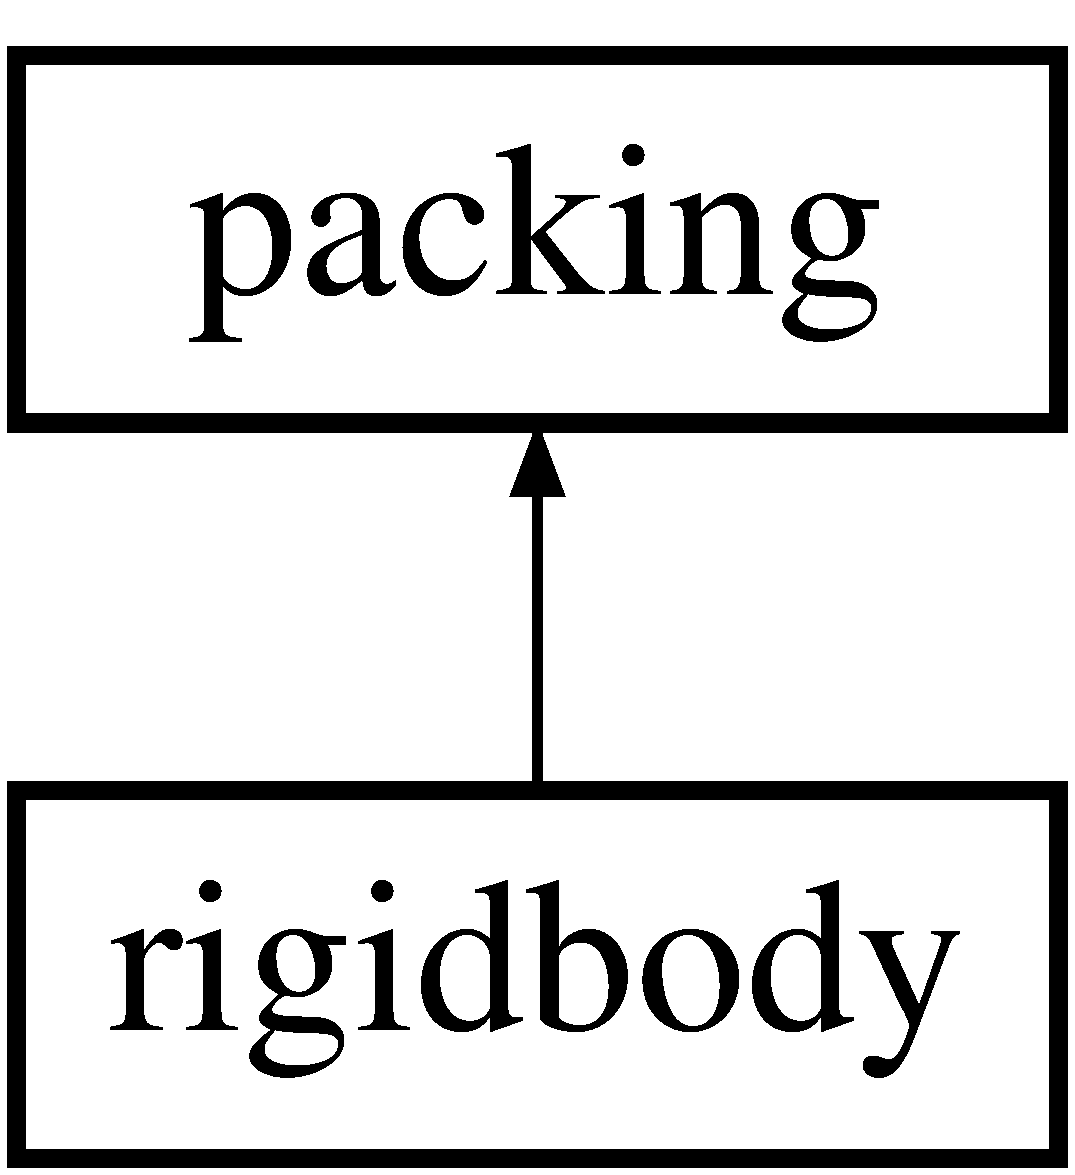
\includegraphics[height=2.000000cm]{classrigidbody}
\end{center}
\end{figure}
\subsection*{Public Member Functions}
\begin{DoxyCompactItemize}
\item 
\mbox{\hyperlink{classrigidbody_a2d1f12365075606f81a18c3ce9454246}{rigidbody}} (string \&rbstr, int n, int dof, int nc, int s)
\item 
\mbox{\hyperlink{classrigidbody_a70821dc58b283f257e84016962f06381}{$\sim$rigidbody}} ()
\item 
void \mbox{\hyperlink{classrigidbody_a3e81aee584c1f57c729d68000637df37}{reset\+\_\+cm}} ()
\item 
void \mbox{\hyperlink{classrigidbody_af5b3f78c77e8535e2d3f065f66225d3c}{update\+\_\+phi}} ()
\item 
void \mbox{\hyperlink{classrigidbody_a30fc1a6f7cc98cee01b1a0b284c9a461}{update\+\_\+euler}} ()
\item 
int \mbox{\hyperlink{classrigidbody_a9287ef3ed29115edff7a823300b7623d}{get\+\_\+ac\+\_\+sum}} ()
\item 
double \mbox{\hyperlink{classrigidbody_ab60de6c5a1f3595ab4b6c87a2518acf6}{get\+\_\+atomic\+\_\+distance}} (int i, int j, int ai, int aj, double aij\mbox{[}$\,$\mbox{]})
\item 
double \mbox{\hyperlink{classrigidbody_afdbc4769886ebdd81947d3f9cdb5a905}{get\+\_\+\+Natot}} ()
\item 
double \mbox{\hyperlink{classrigidbody_ae697251dbe67f538682959ccc7aacec0}{get\+\_\+\+L\+WX}} ()
\item 
double \mbox{\hyperlink{classrigidbody_a922325c42744a3e26fafe69e34c884ab}{get\+\_\+\+L\+WY}} ()
\item 
double \mbox{\hyperlink{classrigidbody_aa97f66b8147830cf83b2298ab8c2b286}{get\+\_\+\+L\+WZ}} ()
\item 
void \mbox{\hyperlink{classrigidbody_a0f3f1cbb05a92009e5831e657ee608cc}{get\+\_\+file\+\_\+header}} (string \&rbstr)
\item 
void \mbox{\hyperlink{classrigidbody_a948adf54e71037640543643bbfd1a7c5}{initialize\+\_\+particles}} ()
\item 
void \mbox{\hyperlink{classrigidbody_a41b996f7b9d8064b3c14a2613293873c}{initialize\+\_\+dynamics}} ()
\item 
void \mbox{\hyperlink{classrigidbody_a84c05d9190b4cab031ca9ab7cd18cd9e}{read\+\_\+in\+\_\+info}} (string \&rbstr)
\item 
void \mbox{\hyperlink{classrigidbody_ae4020098663edf7350e3f7061dacb82a}{initialize\+\_\+quaternions}} ()
\item 
void \mbox{\hyperlink{classrigidbody_a4367ebfbba9658e93277b388c346ef6d}{q\+\_\+step}} ()
\item 
void \mbox{\hyperlink{classrigidbody_ab0dbd8ea400ec317677675c6298d1243}{rotation\+\_\+\+W2M}} ()
\item 
void \mbox{\hyperlink{classrigidbody_a0329c2b25c20317b7e869e35adc27b0a}{euler\+\_\+q}} ()
\item 
void \mbox{\hyperlink{classrigidbody_a839b5b063891c8fc71ad3dd990cfbf4a}{pos\+\_\+frot}} ()
\item 
void \mbox{\hyperlink{classrigidbody_aff843c0c9e358e2d33b0c7ff02c37573}{pos\+\_\+brot}} ()
\item 
void \mbox{\hyperlink{classrigidbody_a0855a20a0df2aa086f24f2a383cf8189}{free\+\_\+md}} (double tmp0, double tend)
\item 
void \mbox{\hyperlink{classrigidbody_adcb984a4d69585e1c617d9506218ac9c}{free\+\_\+fire}} (double tmp0, double tend)
\item 
void \mbox{\hyperlink{classrigidbody_afabb8a8ca32317fc8fdb534932e0de88}{verlet\+\_\+first}} ()
\item 
void \mbox{\hyperlink{classrigidbody_a284a5d8bbc75fe6fd81217c6f861ae60}{verlet\+\_\+second}} ()
\item 
void \mbox{\hyperlink{classrigidbody_a6fd9a15863ae304469f28e4ef7274058}{force\+\_\+update}} ()
\item 
int \mbox{\hyperlink{classrigidbody_a8bb19f9f20480add2468b3b9376f7e7a}{rmv\+\_\+rattlers}} (int \&krcrs)
\item 
int \mbox{\hyperlink{classrigidbody_a69d75bd6de90bb5b9a446b8aa23741de}{id\+\_\+rattlers}} ()
\item 
void \mbox{\hyperlink{classrigidbody_ab2d23acd630aa36261f68b7c01ce3dd4}{rb\+\_\+jamming\+\_\+finder}} (double tmp0, int NT, double dphi, double Utol, double Ktol)
\item 
void \mbox{\hyperlink{classrigidbody_aede3f62a6b910a9bc10641de08a1f329}{rb\+\_\+scale}} (double phinew)
\item 
void \mbox{\hyperlink{classrigidbody_ace2c7ef24606c9912fd004a293569b6c}{rb\+\_\+root\+\_\+search}} (double \&phiH, double \&phiL, int \&check\+\_\+rattlers, int epconst, int \mbox{\hyperlink{classpacking_a31eede3d604c45fef6021170ee506c77}{nr}}, double dphi0, double Ktol, double Utol, int t)
\item 
void \mbox{\hyperlink{classrigidbody_a11a83ecf91f922faff8e2f26c8eace54}{rb\+\_\+fire}} ()
\item 
void \mbox{\hyperlink{classrigidbody_aa00fc3768317e6852643a37cbe19c76a}{print\+\_\+stat}} ()
\item 
void \mbox{\hyperlink{classrigidbody_a24ffb7711348dc2813b8c07e899d065f}{print\+\_\+ac}} (std\+::ofstream \&obj, int w)
\item 
void \mbox{\hyperlink{classrigidbody_aa486e3fa6409f5031188193e37eadc10}{print\+\_\+config}} ()
\item 
void \mbox{\hyperlink{classrigidbody_aecb6c9283be568ba2c303d82d174d987}{monitor\+\_\+scale}} (double dphi, double phiL, double phiH)
\item 
void \mbox{\hyperlink{classrigidbody_a0af56b5a8e3c6550c9a45b6a59c262ef}{rigidbody\+\_\+md\+\_\+monitor}} ()
\item 
void \mbox{\hyperlink{classrigidbody_a05123548826f40f3737bd9f0fce21a85}{rigidbody\+\_\+xyz}} ()
\item 
void \mbox{\hyperlink{classrigidbody_ae7af1f93b40b47c9e855bcb0adb74434}{rigidbody\+\_\+print\+\_\+vars}} ()
\end{DoxyCompactItemize}
\subsection*{Additional Inherited Members}


\subsection{Detailed Description}
The rigidbody class inherits from the packing class and contains functionality to simulate a packing experiement consisting of rigidbodies. 

Definition at line 17 of file rigidbody.\+h.



\subsection{Constructor \& Destructor Documentation}
\mbox{\Hypertarget{classrigidbody_a2d1f12365075606f81a18c3ce9454246}\label{classrigidbody_a2d1f12365075606f81a18c3ce9454246}} 
\index{rigidbody@{rigidbody}!rigidbody@{rigidbody}}
\index{rigidbody@{rigidbody}!rigidbody@{rigidbody}}
\subsubsection{\texorpdfstring{rigidbody()}{rigidbody()}}
{\footnotesize\ttfamily rigidbody\+::rigidbody (\begin{DoxyParamCaption}\item[{string \&}]{rbstr,  }\item[{int}]{n,  }\item[{int}]{dof,  }\item[{int}]{nc,  }\item[{int}]{s }\end{DoxyParamCaption})}



Definition at line 36 of file rigidbody.\+cpp.

\mbox{\Hypertarget{classrigidbody_a70821dc58b283f257e84016962f06381}\label{classrigidbody_a70821dc58b283f257e84016962f06381}} 
\index{rigidbody@{rigidbody}!````~rigidbody@{$\sim$rigidbody}}
\index{````~rigidbody@{$\sim$rigidbody}!rigidbody@{rigidbody}}
\subsubsection{\texorpdfstring{$\sim$rigidbody()}{~rigidbody()}}
{\footnotesize\ttfamily rigidbody\+::$\sim$rigidbody (\begin{DoxyParamCaption}{ }\end{DoxyParamCaption})}



Definition at line 72 of file rigidbody.\+cpp.



\subsection{Member Function Documentation}
\mbox{\Hypertarget{classrigidbody_a0329c2b25c20317b7e869e35adc27b0a}\label{classrigidbody_a0329c2b25c20317b7e869e35adc27b0a}} 
\index{rigidbody@{rigidbody}!euler\+\_\+q@{euler\+\_\+q}}
\index{euler\+\_\+q@{euler\+\_\+q}!rigidbody@{rigidbody}}
\subsubsection{\texorpdfstring{euler\+\_\+q()}{euler\_q()}}
{\footnotesize\ttfamily void rigidbody\+::euler\+\_\+q (\begin{DoxyParamCaption}{ }\end{DoxyParamCaption})}



Definition at line 813 of file rigidbody.\+cpp.

\mbox{\Hypertarget{classrigidbody_a6fd9a15863ae304469f28e4ef7274058}\label{classrigidbody_a6fd9a15863ae304469f28e4ef7274058}} 
\index{rigidbody@{rigidbody}!force\+\_\+update@{force\+\_\+update}}
\index{force\+\_\+update@{force\+\_\+update}!rigidbody@{rigidbody}}
\subsubsection{\texorpdfstring{force\+\_\+update()}{force\_update()}}
{\footnotesize\ttfamily void rigidbody\+::force\+\_\+update (\begin{DoxyParamCaption}{ }\end{DoxyParamCaption})}



Definition at line 972 of file rigidbody.\+cpp.

\mbox{\Hypertarget{classrigidbody_adcb984a4d69585e1c617d9506218ac9c}\label{classrigidbody_adcb984a4d69585e1c617d9506218ac9c}} 
\index{rigidbody@{rigidbody}!free\+\_\+fire@{free\+\_\+fire}}
\index{free\+\_\+fire@{free\+\_\+fire}!rigidbody@{rigidbody}}
\subsubsection{\texorpdfstring{free\+\_\+fire()}{free\_fire()}}
{\footnotesize\ttfamily void rigidbody\+::free\+\_\+fire (\begin{DoxyParamCaption}\item[{double}]{tmp0,  }\item[{double}]{tend }\end{DoxyParamCaption})}



Definition at line 558 of file rigidbody.\+cpp.

\mbox{\Hypertarget{classrigidbody_a0855a20a0df2aa086f24f2a383cf8189}\label{classrigidbody_a0855a20a0df2aa086f24f2a383cf8189}} 
\index{rigidbody@{rigidbody}!free\+\_\+md@{free\+\_\+md}}
\index{free\+\_\+md@{free\+\_\+md}!rigidbody@{rigidbody}}
\subsubsection{\texorpdfstring{free\+\_\+md()}{free\_md()}}
{\footnotesize\ttfamily void rigidbody\+::free\+\_\+md (\begin{DoxyParamCaption}\item[{double}]{tmp0,  }\item[{double}]{tend }\end{DoxyParamCaption})}



Definition at line 506 of file rigidbody.\+cpp.

\mbox{\Hypertarget{classrigidbody_a9287ef3ed29115edff7a823300b7623d}\label{classrigidbody_a9287ef3ed29115edff7a823300b7623d}} 
\index{rigidbody@{rigidbody}!get\+\_\+ac\+\_\+sum@{get\+\_\+ac\+\_\+sum}}
\index{get\+\_\+ac\+\_\+sum@{get\+\_\+ac\+\_\+sum}!rigidbody@{rigidbody}}
\subsubsection{\texorpdfstring{get\+\_\+ac\+\_\+sum()}{get\_ac\_sum()}}
{\footnotesize\ttfamily int rigidbody\+::get\+\_\+ac\+\_\+sum (\begin{DoxyParamCaption}{ }\end{DoxyParamCaption})}



Definition at line 187 of file rigidbody.\+cpp.

\mbox{\Hypertarget{classrigidbody_ab60de6c5a1f3595ab4b6c87a2518acf6}\label{classrigidbody_ab60de6c5a1f3595ab4b6c87a2518acf6}} 
\index{rigidbody@{rigidbody}!get\+\_\+atomic\+\_\+distance@{get\+\_\+atomic\+\_\+distance}}
\index{get\+\_\+atomic\+\_\+distance@{get\+\_\+atomic\+\_\+distance}!rigidbody@{rigidbody}}
\subsubsection{\texorpdfstring{get\+\_\+atomic\+\_\+distance()}{get\_atomic\_distance()}}
{\footnotesize\ttfamily double rigidbody\+::get\+\_\+atomic\+\_\+distance (\begin{DoxyParamCaption}\item[{int}]{i,  }\item[{int}]{j,  }\item[{int}]{ai,  }\item[{int}]{aj,  }\item[{double}]{aij\mbox{[}$\,$\mbox{]} }\end{DoxyParamCaption})}



Definition at line 195 of file rigidbody.\+cpp.

\mbox{\Hypertarget{classrigidbody_a0f3f1cbb05a92009e5831e657ee608cc}\label{classrigidbody_a0f3f1cbb05a92009e5831e657ee608cc}} 
\index{rigidbody@{rigidbody}!get\+\_\+file\+\_\+header@{get\+\_\+file\+\_\+header}}
\index{get\+\_\+file\+\_\+header@{get\+\_\+file\+\_\+header}!rigidbody@{rigidbody}}
\subsubsection{\texorpdfstring{get\+\_\+file\+\_\+header()}{get\_file\_header()}}
{\footnotesize\ttfamily void rigidbody\+::get\+\_\+file\+\_\+header (\begin{DoxyParamCaption}\item[{string \&}]{rbstr }\end{DoxyParamCaption})}



Definition at line 268 of file rigidbody.\+cpp.

\mbox{\Hypertarget{classrigidbody_ae697251dbe67f538682959ccc7aacec0}\label{classrigidbody_ae697251dbe67f538682959ccc7aacec0}} 
\index{rigidbody@{rigidbody}!get\+\_\+\+L\+WX@{get\+\_\+\+L\+WX}}
\index{get\+\_\+\+L\+WX@{get\+\_\+\+L\+WX}!rigidbody@{rigidbody}}
\subsubsection{\texorpdfstring{get\+\_\+\+L\+W\+X()}{get\_LWX()}}
{\footnotesize\ttfamily double rigidbody\+::get\+\_\+\+L\+WX (\begin{DoxyParamCaption}{ }\end{DoxyParamCaption})}



Definition at line 229 of file rigidbody.\+cpp.

\mbox{\Hypertarget{classrigidbody_a922325c42744a3e26fafe69e34c884ab}\label{classrigidbody_a922325c42744a3e26fafe69e34c884ab}} 
\index{rigidbody@{rigidbody}!get\+\_\+\+L\+WY@{get\+\_\+\+L\+WY}}
\index{get\+\_\+\+L\+WY@{get\+\_\+\+L\+WY}!rigidbody@{rigidbody}}
\subsubsection{\texorpdfstring{get\+\_\+\+L\+W\+Y()}{get\_LWY()}}
{\footnotesize\ttfamily double rigidbody\+::get\+\_\+\+L\+WY (\begin{DoxyParamCaption}{ }\end{DoxyParamCaption})}



Definition at line 239 of file rigidbody.\+cpp.

\mbox{\Hypertarget{classrigidbody_aa97f66b8147830cf83b2298ab8c2b286}\label{classrigidbody_aa97f66b8147830cf83b2298ab8c2b286}} 
\index{rigidbody@{rigidbody}!get\+\_\+\+L\+WZ@{get\+\_\+\+L\+WZ}}
\index{get\+\_\+\+L\+WZ@{get\+\_\+\+L\+WZ}!rigidbody@{rigidbody}}
\subsubsection{\texorpdfstring{get\+\_\+\+L\+W\+Z()}{get\_LWZ()}}
{\footnotesize\ttfamily double rigidbody\+::get\+\_\+\+L\+WZ (\begin{DoxyParamCaption}{ }\end{DoxyParamCaption})}



Definition at line 249 of file rigidbody.\+cpp.

\mbox{\Hypertarget{classrigidbody_afdbc4769886ebdd81947d3f9cdb5a905}\label{classrigidbody_afdbc4769886ebdd81947d3f9cdb5a905}} 
\index{rigidbody@{rigidbody}!get\+\_\+\+Natot@{get\+\_\+\+Natot}}
\index{get\+\_\+\+Natot@{get\+\_\+\+Natot}!rigidbody@{rigidbody}}
\subsubsection{\texorpdfstring{get\+\_\+\+Natot()}{get\_Natot()}}
{\footnotesize\ttfamily double rigidbody\+::get\+\_\+\+Natot (\begin{DoxyParamCaption}{ }\end{DoxyParamCaption})}



Definition at line 219 of file rigidbody.\+cpp.

\mbox{\Hypertarget{classrigidbody_a69d75bd6de90bb5b9a446b8aa23741de}\label{classrigidbody_a69d75bd6de90bb5b9a446b8aa23741de}} 
\index{rigidbody@{rigidbody}!id\+\_\+rattlers@{id\+\_\+rattlers}}
\index{id\+\_\+rattlers@{id\+\_\+rattlers}!rigidbody@{rigidbody}}
\subsubsection{\texorpdfstring{id\+\_\+rattlers()}{id\_rattlers()}}
{\footnotesize\ttfamily int rigidbody\+::id\+\_\+rattlers (\begin{DoxyParamCaption}{ }\end{DoxyParamCaption})}



Definition at line 1261 of file rigidbody.\+cpp.

\mbox{\Hypertarget{classrigidbody_a41b996f7b9d8064b3c14a2613293873c}\label{classrigidbody_a41b996f7b9d8064b3c14a2613293873c}} 
\index{rigidbody@{rigidbody}!initialize\+\_\+dynamics@{initialize\+\_\+dynamics}}
\index{initialize\+\_\+dynamics@{initialize\+\_\+dynamics}!rigidbody@{rigidbody}}
\subsubsection{\texorpdfstring{initialize\+\_\+dynamics()}{initialize\_dynamics()}}
{\footnotesize\ttfamily void rigidbody\+::initialize\+\_\+dynamics (\begin{DoxyParamCaption}{ }\end{DoxyParamCaption})}



Definition at line 368 of file rigidbody.\+cpp.

\mbox{\Hypertarget{classrigidbody_a948adf54e71037640543643bbfd1a7c5}\label{classrigidbody_a948adf54e71037640543643bbfd1a7c5}} 
\index{rigidbody@{rigidbody}!initialize\+\_\+particles@{initialize\+\_\+particles}}
\index{initialize\+\_\+particles@{initialize\+\_\+particles}!rigidbody@{rigidbody}}
\subsubsection{\texorpdfstring{initialize\+\_\+particles()}{initialize\_particles()}}
{\footnotesize\ttfamily void rigidbody\+::initialize\+\_\+particles (\begin{DoxyParamCaption}{ }\end{DoxyParamCaption})}



Definition at line 326 of file rigidbody.\+cpp.

\mbox{\Hypertarget{classrigidbody_ae4020098663edf7350e3f7061dacb82a}\label{classrigidbody_ae4020098663edf7350e3f7061dacb82a}} 
\index{rigidbody@{rigidbody}!initialize\+\_\+quaternions@{initialize\+\_\+quaternions}}
\index{initialize\+\_\+quaternions@{initialize\+\_\+quaternions}!rigidbody@{rigidbody}}
\subsubsection{\texorpdfstring{initialize\+\_\+quaternions()}{initialize\_quaternions()}}
{\footnotesize\ttfamily void rigidbody\+::initialize\+\_\+quaternions (\begin{DoxyParamCaption}{ }\end{DoxyParamCaption})}



Definition at line 481 of file rigidbody.\+cpp.

\mbox{\Hypertarget{classrigidbody_aecb6c9283be568ba2c303d82d174d987}\label{classrigidbody_aecb6c9283be568ba2c303d82d174d987}} 
\index{rigidbody@{rigidbody}!monitor\+\_\+scale@{monitor\+\_\+scale}}
\index{monitor\+\_\+scale@{monitor\+\_\+scale}!rigidbody@{rigidbody}}
\subsubsection{\texorpdfstring{monitor\+\_\+scale()}{monitor\_scale()}}
{\footnotesize\ttfamily void rigidbody\+::monitor\+\_\+scale (\begin{DoxyParamCaption}\item[{double}]{dphi,  }\item[{double}]{phiL,  }\item[{double}]{phiH }\end{DoxyParamCaption})}



Definition at line 1768 of file rigidbody.\+cpp.

\mbox{\Hypertarget{classrigidbody_aff843c0c9e358e2d33b0c7ff02c37573}\label{classrigidbody_aff843c0c9e358e2d33b0c7ff02c37573}} 
\index{rigidbody@{rigidbody}!pos\+\_\+brot@{pos\+\_\+brot}}
\index{pos\+\_\+brot@{pos\+\_\+brot}!rigidbody@{rigidbody}}
\subsubsection{\texorpdfstring{pos\+\_\+brot()}{pos\_brot()}}
{\footnotesize\ttfamily void rigidbody\+::pos\+\_\+brot (\begin{DoxyParamCaption}{ }\end{DoxyParamCaption})}



Definition at line 945 of file rigidbody.\+cpp.

\mbox{\Hypertarget{classrigidbody_a839b5b063891c8fc71ad3dd990cfbf4a}\label{classrigidbody_a839b5b063891c8fc71ad3dd990cfbf4a}} 
\index{rigidbody@{rigidbody}!pos\+\_\+frot@{pos\+\_\+frot}}
\index{pos\+\_\+frot@{pos\+\_\+frot}!rigidbody@{rigidbody}}
\subsubsection{\texorpdfstring{pos\+\_\+frot()}{pos\_frot()}}
{\footnotesize\ttfamily void rigidbody\+::pos\+\_\+frot (\begin{DoxyParamCaption}{ }\end{DoxyParamCaption})}



Definition at line 919 of file rigidbody.\+cpp.

\mbox{\Hypertarget{classrigidbody_a24ffb7711348dc2813b8c07e899d065f}\label{classrigidbody_a24ffb7711348dc2813b8c07e899d065f}} 
\index{rigidbody@{rigidbody}!print\+\_\+ac@{print\+\_\+ac}}
\index{print\+\_\+ac@{print\+\_\+ac}!rigidbody@{rigidbody}}
\subsubsection{\texorpdfstring{print\+\_\+ac()}{print\_ac()}}
{\footnotesize\ttfamily void rigidbody\+::print\+\_\+ac (\begin{DoxyParamCaption}\item[{std\+::ofstream \&}]{obj,  }\item[{int}]{w }\end{DoxyParamCaption})}



Definition at line 1647 of file rigidbody.\+cpp.

\mbox{\Hypertarget{classrigidbody_aa486e3fa6409f5031188193e37eadc10}\label{classrigidbody_aa486e3fa6409f5031188193e37eadc10}} 
\index{rigidbody@{rigidbody}!print\+\_\+config@{print\+\_\+config}}
\index{print\+\_\+config@{print\+\_\+config}!rigidbody@{rigidbody}}
\subsubsection{\texorpdfstring{print\+\_\+config()}{print\_config()}}
{\footnotesize\ttfamily void rigidbody\+::print\+\_\+config (\begin{DoxyParamCaption}{ }\end{DoxyParamCaption})}



Definition at line 1654 of file rigidbody.\+cpp.

\mbox{\Hypertarget{classrigidbody_aa00fc3768317e6852643a37cbe19c76a}\label{classrigidbody_aa00fc3768317e6852643a37cbe19c76a}} 
\index{rigidbody@{rigidbody}!print\+\_\+stat@{print\+\_\+stat}}
\index{print\+\_\+stat@{print\+\_\+stat}!rigidbody@{rigidbody}}
\subsubsection{\texorpdfstring{print\+\_\+stat()}{print\_stat()}}
{\footnotesize\ttfamily void rigidbody\+::print\+\_\+stat (\begin{DoxyParamCaption}{ }\end{DoxyParamCaption})}



Definition at line 1611 of file rigidbody.\+cpp.

\mbox{\Hypertarget{classrigidbody_a4367ebfbba9658e93277b388c346ef6d}\label{classrigidbody_a4367ebfbba9658e93277b388c346ef6d}} 
\index{rigidbody@{rigidbody}!q\+\_\+step@{q\+\_\+step}}
\index{q\+\_\+step@{q\+\_\+step}!rigidbody@{rigidbody}}
\subsubsection{\texorpdfstring{q\+\_\+step()}{q\_step()}}
{\footnotesize\ttfamily void rigidbody\+::q\+\_\+step (\begin{DoxyParamCaption}{ }\end{DoxyParamCaption})}



Definition at line 758 of file rigidbody.\+cpp.

\mbox{\Hypertarget{classrigidbody_a11a83ecf91f922faff8e2f26c8eace54}\label{classrigidbody_a11a83ecf91f922faff8e2f26c8eace54}} 
\index{rigidbody@{rigidbody}!rb\+\_\+fire@{rb\+\_\+fire}}
\index{rb\+\_\+fire@{rb\+\_\+fire}!rigidbody@{rigidbody}}
\subsubsection{\texorpdfstring{rb\+\_\+fire()}{rb\_fire()}}
{\footnotesize\ttfamily void rigidbody\+::rb\+\_\+fire (\begin{DoxyParamCaption}{ }\end{DoxyParamCaption})}



Definition at line 1318 of file rigidbody.\+cpp.

\mbox{\Hypertarget{classrigidbody_ab2d23acd630aa36261f68b7c01ce3dd4}\label{classrigidbody_ab2d23acd630aa36261f68b7c01ce3dd4}} 
\index{rigidbody@{rigidbody}!rb\+\_\+jamming\+\_\+finder@{rb\+\_\+jamming\+\_\+finder}}
\index{rb\+\_\+jamming\+\_\+finder@{rb\+\_\+jamming\+\_\+finder}!rigidbody@{rigidbody}}
\subsubsection{\texorpdfstring{rb\+\_\+jamming\+\_\+finder()}{rb\_jamming\_finder()}}
{\footnotesize\ttfamily void rigidbody\+::rb\+\_\+jamming\+\_\+finder (\begin{DoxyParamCaption}\item[{double}]{tmp0,  }\item[{int}]{NT,  }\item[{double}]{dphi,  }\item[{double}]{Utol,  }\item[{double}]{Ktol }\end{DoxyParamCaption})}



Definition at line 619 of file rigidbody.\+cpp.

\mbox{\Hypertarget{classrigidbody_ace2c7ef24606c9912fd004a293569b6c}\label{classrigidbody_ace2c7ef24606c9912fd004a293569b6c}} 
\index{rigidbody@{rigidbody}!rb\+\_\+root\+\_\+search@{rb\+\_\+root\+\_\+search}}
\index{rb\+\_\+root\+\_\+search@{rb\+\_\+root\+\_\+search}!rigidbody@{rigidbody}}
\subsubsection{\texorpdfstring{rb\+\_\+root\+\_\+search()}{rb\_root\_search()}}
{\footnotesize\ttfamily void rigidbody\+::rb\+\_\+root\+\_\+search (\begin{DoxyParamCaption}\item[{double \&}]{phiH,  }\item[{double \&}]{phiL,  }\item[{int \&}]{check\+\_\+rattlers,  }\item[{int}]{epconst,  }\item[{int}]{nr,  }\item[{double}]{dphi0,  }\item[{double}]{Ktol,  }\item[{double}]{Utol,  }\item[{int}]{t }\end{DoxyParamCaption})}



Definition at line 1420 of file rigidbody.\+cpp.

\mbox{\Hypertarget{classrigidbody_aede3f62a6b910a9bc10641de08a1f329}\label{classrigidbody_aede3f62a6b910a9bc10641de08a1f329}} 
\index{rigidbody@{rigidbody}!rb\+\_\+scale@{rb\+\_\+scale}}
\index{rb\+\_\+scale@{rb\+\_\+scale}!rigidbody@{rigidbody}}
\subsubsection{\texorpdfstring{rb\+\_\+scale()}{rb\_scale()}}
{\footnotesize\ttfamily void rigidbody\+::rb\+\_\+scale (\begin{DoxyParamCaption}\item[{double}]{phinew }\end{DoxyParamCaption})}



Definition at line 1275 of file rigidbody.\+cpp.

\mbox{\Hypertarget{classrigidbody_a84c05d9190b4cab031ca9ab7cd18cd9e}\label{classrigidbody_a84c05d9190b4cab031ca9ab7cd18cd9e}} 
\index{rigidbody@{rigidbody}!read\+\_\+in\+\_\+info@{read\+\_\+in\+\_\+info}}
\index{read\+\_\+in\+\_\+info@{read\+\_\+in\+\_\+info}!rigidbody@{rigidbody}}
\subsubsection{\texorpdfstring{read\+\_\+in\+\_\+info()}{read\_in\_info()}}
{\footnotesize\ttfamily void rigidbody\+::read\+\_\+in\+\_\+info (\begin{DoxyParamCaption}\item[{string \&}]{rbstr }\end{DoxyParamCaption})}



Definition at line 415 of file rigidbody.\+cpp.

\mbox{\Hypertarget{classrigidbody_a3e81aee584c1f57c729d68000637df37}\label{classrigidbody_a3e81aee584c1f57c729d68000637df37}} 
\index{rigidbody@{rigidbody}!reset\+\_\+cm@{reset\+\_\+cm}}
\index{reset\+\_\+cm@{reset\+\_\+cm}!rigidbody@{rigidbody}}
\subsubsection{\texorpdfstring{reset\+\_\+cm()}{reset\_cm()}}
{\footnotesize\ttfamily void rigidbody\+::reset\+\_\+cm (\begin{DoxyParamCaption}{ }\end{DoxyParamCaption})}



Definition at line 148 of file rigidbody.\+cpp.

\mbox{\Hypertarget{classrigidbody_a0af56b5a8e3c6550c9a45b6a59c262ef}\label{classrigidbody_a0af56b5a8e3c6550c9a45b6a59c262ef}} 
\index{rigidbody@{rigidbody}!rigidbody\+\_\+md\+\_\+monitor@{rigidbody\+\_\+md\+\_\+monitor}}
\index{rigidbody\+\_\+md\+\_\+monitor@{rigidbody\+\_\+md\+\_\+monitor}!rigidbody@{rigidbody}}
\subsubsection{\texorpdfstring{rigidbody\+\_\+md\+\_\+monitor()}{rigidbody\_md\_monitor()}}
{\footnotesize\ttfamily void rigidbody\+::rigidbody\+\_\+md\+\_\+monitor (\begin{DoxyParamCaption}{ }\end{DoxyParamCaption})}



Definition at line 1718 of file rigidbody.\+cpp.

\mbox{\Hypertarget{classrigidbody_ae7af1f93b40b47c9e855bcb0adb74434}\label{classrigidbody_ae7af1f93b40b47c9e855bcb0adb74434}} 
\index{rigidbody@{rigidbody}!rigidbody\+\_\+print\+\_\+vars@{rigidbody\+\_\+print\+\_\+vars}}
\index{rigidbody\+\_\+print\+\_\+vars@{rigidbody\+\_\+print\+\_\+vars}!rigidbody@{rigidbody}}
\subsubsection{\texorpdfstring{rigidbody\+\_\+print\+\_\+vars()}{rigidbody\_print\_vars()}}
{\footnotesize\ttfamily void rigidbody\+::rigidbody\+\_\+print\+\_\+vars (\begin{DoxyParamCaption}{ }\end{DoxyParamCaption})}



Definition at line 1866 of file rigidbody.\+cpp.

\mbox{\Hypertarget{classrigidbody_a05123548826f40f3737bd9f0fce21a85}\label{classrigidbody_a05123548826f40f3737bd9f0fce21a85}} 
\index{rigidbody@{rigidbody}!rigidbody\+\_\+xyz@{rigidbody\+\_\+xyz}}
\index{rigidbody\+\_\+xyz@{rigidbody\+\_\+xyz}!rigidbody@{rigidbody}}
\subsubsection{\texorpdfstring{rigidbody\+\_\+xyz()}{rigidbody\_xyz()}}
{\footnotesize\ttfamily void rigidbody\+::rigidbody\+\_\+xyz (\begin{DoxyParamCaption}{ }\end{DoxyParamCaption})}



Definition at line 1779 of file rigidbody.\+cpp.

\mbox{\Hypertarget{classrigidbody_a8bb19f9f20480add2468b3b9376f7e7a}\label{classrigidbody_a8bb19f9f20480add2468b3b9376f7e7a}} 
\index{rigidbody@{rigidbody}!rmv\+\_\+rattlers@{rmv\+\_\+rattlers}}
\index{rmv\+\_\+rattlers@{rmv\+\_\+rattlers}!rigidbody@{rigidbody}}
\subsubsection{\texorpdfstring{rmv\+\_\+rattlers()}{rmv\_rattlers()}}
{\footnotesize\ttfamily int rigidbody\+::rmv\+\_\+rattlers (\begin{DoxyParamCaption}\item[{int \&}]{krcrs }\end{DoxyParamCaption})}



Definition at line 1194 of file rigidbody.\+cpp.

\mbox{\Hypertarget{classrigidbody_ab0dbd8ea400ec317677675c6298d1243}\label{classrigidbody_ab0dbd8ea400ec317677675c6298d1243}} 
\index{rigidbody@{rigidbody}!rotation\+\_\+\+W2M@{rotation\+\_\+\+W2M}}
\index{rotation\+\_\+\+W2M@{rotation\+\_\+\+W2M}!rigidbody@{rigidbody}}
\subsubsection{\texorpdfstring{rotation\+\_\+\+W2\+M()}{rotation\_W2M()}}
{\footnotesize\ttfamily void rigidbody\+::rotation\+\_\+\+W2M (\begin{DoxyParamCaption}{ }\end{DoxyParamCaption})}



Definition at line 769 of file rigidbody.\+cpp.

\mbox{\Hypertarget{classrigidbody_a30fc1a6f7cc98cee01b1a0b284c9a461}\label{classrigidbody_a30fc1a6f7cc98cee01b1a0b284c9a461}} 
\index{rigidbody@{rigidbody}!update\+\_\+euler@{update\+\_\+euler}}
\index{update\+\_\+euler@{update\+\_\+euler}!rigidbody@{rigidbody}}
\subsubsection{\texorpdfstring{update\+\_\+euler()}{update\_euler()}}
{\footnotesize\ttfamily void rigidbody\+::update\+\_\+euler (\begin{DoxyParamCaption}{ }\end{DoxyParamCaption})}



Definition at line 169 of file rigidbody.\+cpp.

\mbox{\Hypertarget{classrigidbody_af5b3f78c77e8535e2d3f065f66225d3c}\label{classrigidbody_af5b3f78c77e8535e2d3f065f66225d3c}} 
\index{rigidbody@{rigidbody}!update\+\_\+phi@{update\+\_\+phi}}
\index{update\+\_\+phi@{update\+\_\+phi}!rigidbody@{rigidbody}}
\subsubsection{\texorpdfstring{update\+\_\+phi()}{update\_phi()}}
{\footnotesize\ttfamily void rigidbody\+::update\+\_\+phi (\begin{DoxyParamCaption}{ }\end{DoxyParamCaption})}



Definition at line 155 of file rigidbody.\+cpp.

\mbox{\Hypertarget{classrigidbody_afabb8a8ca32317fc8fdb534932e0de88}\label{classrigidbody_afabb8a8ca32317fc8fdb534932e0de88}} 
\index{rigidbody@{rigidbody}!verlet\+\_\+first@{verlet\+\_\+first}}
\index{verlet\+\_\+first@{verlet\+\_\+first}!rigidbody@{rigidbody}}
\subsubsection{\texorpdfstring{verlet\+\_\+first()}{verlet\_first()}}
{\footnotesize\ttfamily void rigidbody\+::verlet\+\_\+first (\begin{DoxyParamCaption}{ }\end{DoxyParamCaption})}



Definition at line 719 of file rigidbody.\+cpp.

\mbox{\Hypertarget{classrigidbody_a284a5d8bbc75fe6fd81217c6f861ae60}\label{classrigidbody_a284a5d8bbc75fe6fd81217c6f861ae60}} 
\index{rigidbody@{rigidbody}!verlet\+\_\+second@{verlet\+\_\+second}}
\index{verlet\+\_\+second@{verlet\+\_\+second}!rigidbody@{rigidbody}}
\subsubsection{\texorpdfstring{verlet\+\_\+second()}{verlet\_second()}}
{\footnotesize\ttfamily void rigidbody\+::verlet\+\_\+second (\begin{DoxyParamCaption}{ }\end{DoxyParamCaption})}



Definition at line 738 of file rigidbody.\+cpp.



The documentation for this class was generated from the following files\+:\begin{DoxyCompactItemize}
\item 
src/\mbox{\hyperlink{rigidbody_8h}{rigidbody.\+h}}\item 
src/\mbox{\hyperlink{rigidbody_8cpp}{rigidbody.\+cpp}}\end{DoxyCompactItemize}

\chapter{File Documentation}
\hypertarget{homepage_8dox}{}\section{src/homepage.dox File Reference}
\label{homepage_8dox}\index{src/homepage.\+dox@{src/homepage.\+dox}}

\hypertarget{packing_8cpp}{}\section{src/packing.cpp File Reference}
\label{packing_8cpp}\index{src/packing.\+cpp@{src/packing.\+cpp}}
{\ttfamily \#include \char`\"{}packing.\+h\char`\"{}}\newline
{\ttfamily \#include $<$stdio.\+h$>$}\newline
{\ttfamily \#include $<$iostream$>$}\newline
{\ttfamily \#include $<$iomanip$>$}\newline
{\ttfamily \#include $<$fstream$>$}\newline
{\ttfamily \#include $<$stdlib.\+h$>$}\newline
{\ttfamily \#include $<$string$>$}\newline
{\ttfamily \#include $<$cmath$>$}\newline
{\ttfamily \#include $<$vector$>$}\newline
\subsection*{Macros}
\begin{DoxyCompactItemize}
\item 
\#define \mbox{\hyperlink{packing_8cpp_afff2c6be67c226eb2b1359a3cd2042b2}{D\+E\+B\+U\+G\+\_\+\+O\+FF}}
\end{DoxyCompactItemize}
\subsection*{Variables}
\begin{DoxyCompactItemize}
\item 
const double \mbox{\hyperlink{packing_8cpp_a952eac791b596a61bba0a133a3bb439f}{PI}} = 3.\+1415926
\end{DoxyCompactItemize}


\subsection{Macro Definition Documentation}
\mbox{\Hypertarget{packing_8cpp_afff2c6be67c226eb2b1359a3cd2042b2}\label{packing_8cpp_afff2c6be67c226eb2b1359a3cd2042b2}} 
\index{packing.\+cpp@{packing.\+cpp}!D\+E\+B\+U\+G\+\_\+\+O\+FF@{D\+E\+B\+U\+G\+\_\+\+O\+FF}}
\index{D\+E\+B\+U\+G\+\_\+\+O\+FF@{D\+E\+B\+U\+G\+\_\+\+O\+FF}!packing.\+cpp@{packing.\+cpp}}
\subsubsection{\texorpdfstring{D\+E\+B\+U\+G\+\_\+\+O\+FF}{DEBUG\_OFF}}
{\footnotesize\ttfamily \#define D\+E\+B\+U\+G\+\_\+\+O\+FF}



Definition at line 22 of file packing.\+cpp.



\subsection{Variable Documentation}
\mbox{\Hypertarget{packing_8cpp_a952eac791b596a61bba0a133a3bb439f}\label{packing_8cpp_a952eac791b596a61bba0a133a3bb439f}} 
\index{packing.\+cpp@{packing.\+cpp}!PI@{PI}}
\index{PI@{PI}!packing.\+cpp@{packing.\+cpp}}
\subsubsection{\texorpdfstring{PI}{PI}}
{\footnotesize\ttfamily const double PI = 3.\+1415926}



Definition at line 24 of file packing.\+cpp.


\hypertarget{packing_8h}{}\section{src/packing.h File Reference}
\label{packing_8h}\index{src/packing.\+h@{src/packing.\+h}}
{\ttfamily \#include $<$iostream$>$}\newline
{\ttfamily \#include $<$cmath$>$}\newline
{\ttfamily \#include $<$fstream$>$}\newline
{\ttfamily \#include $<$string$>$}\newline
{\ttfamily \#include $<$vector$>$}\newline
\subsection*{Classes}
\begin{DoxyCompactItemize}
\item 
class \mbox{\hyperlink{classpacking}{packing}}
\end{DoxyCompactItemize}

\hypertarget{packing__meas_8cpp}{}\section{src/packing\+\_\+meas.cpp File Reference}
\label{packing__meas_8cpp}\index{src/packing\+\_\+meas.\+cpp@{src/packing\+\_\+meas.\+cpp}}
{\ttfamily \#include \char`\"{}packing.\+h\char`\"{}}\newline
{\ttfamily \#include $<$stdio.\+h$>$}\newline
{\ttfamily \#include $<$iostream$>$}\newline
{\ttfamily \#include $<$iomanip$>$}\newline
{\ttfamily \#include $<$fstream$>$}\newline
{\ttfamily \#include $<$stdlib.\+h$>$}\newline
{\ttfamily \#include $<$string$>$}\newline
{\ttfamily \#include $<$cmath$>$}\newline
{\ttfamily \#include $<$vector$>$}\newline
\subsection*{Variables}
\begin{DoxyCompactItemize}
\item 
const double \mbox{\hyperlink{packing__meas_8cpp_a952eac791b596a61bba0a133a3bb439f}{PI}} = 3.\+1415926
\end{DoxyCompactItemize}


\subsection{Variable Documentation}
\mbox{\Hypertarget{packing__meas_8cpp_a952eac791b596a61bba0a133a3bb439f}\label{packing__meas_8cpp_a952eac791b596a61bba0a133a3bb439f}} 
\index{packing\+\_\+meas.\+cpp@{packing\+\_\+meas.\+cpp}!PI@{PI}}
\index{PI@{PI}!packing\+\_\+meas.\+cpp@{packing\+\_\+meas.\+cpp}}
\subsubsection{\texorpdfstring{PI}{PI}}
{\footnotesize\ttfamily const double PI = 3.\+1415926}



Definition at line 22 of file packing\+\_\+meas.\+cpp.


\hypertarget{packing__sim_8cpp}{}\section{src/packing\+\_\+sim.cpp File Reference}
\label{packing__sim_8cpp}\index{src/packing\+\_\+sim.\+cpp@{src/packing\+\_\+sim.\+cpp}}
{\ttfamily \#include \char`\"{}packing.\+h\char`\"{}}\newline
{\ttfamily \#include $<$stdio.\+h$>$}\newline
{\ttfamily \#include $<$iostream$>$}\newline
{\ttfamily \#include $<$iomanip$>$}\newline
{\ttfamily \#include $<$fstream$>$}\newline
{\ttfamily \#include $<$stdlib.\+h$>$}\newline
{\ttfamily \#include $<$string$>$}\newline
{\ttfamily \#include $<$cmath$>$}\newline
{\ttfamily \#include $<$vector$>$}\newline
\subsection*{Functions}
\begin{DoxyCompactItemize}
\item 
void \mbox{\hyperlink{packing__sim_8cpp_a9ed09732ec9f0a19d770b9ae0f86adaf}{grnf}} (double \&x)
\end{DoxyCompactItemize}
\subsection*{Variables}
\begin{DoxyCompactItemize}
\item 
const double \mbox{\hyperlink{packing__sim_8cpp_a952eac791b596a61bba0a133a3bb439f}{PI}} = 3.\+1415926
\end{DoxyCompactItemize}


\subsection{Function Documentation}
\mbox{\Hypertarget{packing__sim_8cpp_a9ed09732ec9f0a19d770b9ae0f86adaf}\label{packing__sim_8cpp_a9ed09732ec9f0a19d770b9ae0f86adaf}} 
\index{packing\+\_\+sim.\+cpp@{packing\+\_\+sim.\+cpp}!grnf@{grnf}}
\index{grnf@{grnf}!packing\+\_\+sim.\+cpp@{packing\+\_\+sim.\+cpp}}
\subsubsection{\texorpdfstring{grnf()}{grnf()}}
{\footnotesize\ttfamily void grnf (\begin{DoxyParamCaption}\item[{double \&}]{x }\end{DoxyParamCaption})}



Definition at line 75 of file packing\+\_\+sim.\+cpp.



\subsection{Variable Documentation}
\mbox{\Hypertarget{packing__sim_8cpp_a952eac791b596a61bba0a133a3bb439f}\label{packing__sim_8cpp_a952eac791b596a61bba0a133a3bb439f}} 
\index{packing\+\_\+sim.\+cpp@{packing\+\_\+sim.\+cpp}!PI@{PI}}
\index{PI@{PI}!packing\+\_\+sim.\+cpp@{packing\+\_\+sim.\+cpp}}
\subsubsection{\texorpdfstring{PI}{PI}}
{\footnotesize\ttfamily const double PI = 3.\+1415926}



Definition at line 22 of file packing\+\_\+sim.\+cpp.


\hypertarget{packing__test_8cpp}{}\section{src/packing\+\_\+test.cpp File Reference}
\label{packing__test_8cpp}\index{src/packing\+\_\+test.\+cpp@{src/packing\+\_\+test.\+cpp}}
{\ttfamily \#include \char`\"{}packing.\+h\char`\"{}}\newline
{\ttfamily \#include $<$stdio.\+h$>$}\newline
{\ttfamily \#include $<$iostream$>$}\newline
{\ttfamily \#include $<$iomanip$>$}\newline
{\ttfamily \#include $<$fstream$>$}\newline
{\ttfamily \#include $<$stdlib.\+h$>$}\newline
{\ttfamily \#include $<$string$>$}\newline
{\ttfamily \#include $<$cmath$>$}\newline
{\ttfamily \#include $<$vector$>$}\newline
\subsection*{Macros}
\begin{DoxyCompactItemize}
\item 
\#define \mbox{\hyperlink{packing__test_8cpp_afff2c6be67c226eb2b1359a3cd2042b2}{D\+E\+B\+U\+G\+\_\+\+O\+FF}}
\end{DoxyCompactItemize}
\subsection*{Variables}
\begin{DoxyCompactItemize}
\item 
const double \mbox{\hyperlink{packing__test_8cpp_a952eac791b596a61bba0a133a3bb439f}{PI}} = 3.\+1415926
\end{DoxyCompactItemize}


\subsection{Macro Definition Documentation}
\mbox{\Hypertarget{packing__test_8cpp_afff2c6be67c226eb2b1359a3cd2042b2}\label{packing__test_8cpp_afff2c6be67c226eb2b1359a3cd2042b2}} 
\index{packing\+\_\+test.\+cpp@{packing\+\_\+test.\+cpp}!D\+E\+B\+U\+G\+\_\+\+O\+FF@{D\+E\+B\+U\+G\+\_\+\+O\+FF}}
\index{D\+E\+B\+U\+G\+\_\+\+O\+FF@{D\+E\+B\+U\+G\+\_\+\+O\+FF}!packing\+\_\+test.\+cpp@{packing\+\_\+test.\+cpp}}
\subsubsection{\texorpdfstring{D\+E\+B\+U\+G\+\_\+\+O\+FF}{DEBUG\_OFF}}
{\footnotesize\ttfamily \#define D\+E\+B\+U\+G\+\_\+\+O\+FF}



Definition at line 22 of file packing\+\_\+test.\+cpp.



\subsection{Variable Documentation}
\mbox{\Hypertarget{packing__test_8cpp_a952eac791b596a61bba0a133a3bb439f}\label{packing__test_8cpp_a952eac791b596a61bba0a133a3bb439f}} 
\index{packing\+\_\+test.\+cpp@{packing\+\_\+test.\+cpp}!PI@{PI}}
\index{PI@{PI}!packing\+\_\+test.\+cpp@{packing\+\_\+test.\+cpp}}
\subsubsection{\texorpdfstring{PI}{PI}}
{\footnotesize\ttfamily const double PI = 3.\+1415926}



Definition at line 24 of file packing\+\_\+test.\+cpp.


\hypertarget{_quaternion_8cpp}{}\section{src/\+Quaternion.cpp File Reference}
\label{_quaternion_8cpp}\index{src/\+Quaternion.\+cpp@{src/\+Quaternion.\+cpp}}
{\ttfamily \#include \char`\"{}Quaternion.\+h\char`\"{}}\newline
{\ttfamily \#include $<$stdio.\+h$>$}\newline
{\ttfamily \#include $<$iostream$>$}\newline
{\ttfamily \#include $<$stdlib.\+h$>$}\newline
{\ttfamily \#include $<$string$>$}\newline
{\ttfamily \#include $<$cmath$>$}\newline

\hypertarget{_quaternion_8h}{}\section{src/\+Quaternion.h File Reference}
\label{_quaternion_8h}\index{src/\+Quaternion.\+h@{src/\+Quaternion.\+h}}
{\ttfamily \#include $<$iostream$>$}\newline
\subsection*{Classes}
\begin{DoxyCompactItemize}
\item 
class \mbox{\hyperlink{class_quaternion}{Quaternion}}
\end{DoxyCompactItemize}

\hypertarget{rigidbody_8cpp}{}\section{src/rigidbody.cpp File Reference}
\label{rigidbody_8cpp}\index{src/rigidbody.\+cpp@{src/rigidbody.\+cpp}}
{\ttfamily \#include \char`\"{}Quaternion.\+h\char`\"{}}\newline
{\ttfamily \#include \char`\"{}rigidbody.\+h\char`\"{}}\newline
{\ttfamily \#include \char`\"{}packing.\+h\char`\"{}}\newline
{\ttfamily \#include $<$stdio.\+h$>$}\newline
{\ttfamily \#include $<$iostream$>$}\newline
{\ttfamily \#include $<$iomanip$>$}\newline
{\ttfamily \#include $<$fstream$>$}\newline
{\ttfamily \#include $<$stdlib.\+h$>$}\newline
{\ttfamily \#include $<$string$>$}\newline
{\ttfamily \#include $<$cmath$>$}\newline
{\ttfamily \#include $<$vector$>$}\newline
\subsection*{Macros}
\begin{DoxyCompactItemize}
\item 
\#define \mbox{\hyperlink{rigidbody_8cpp_afff2c6be67c226eb2b1359a3cd2042b2}{D\+E\+B\+U\+G\+\_\+\+O\+FF}}
\end{DoxyCompactItemize}
\subsection*{Variables}
\begin{DoxyCompactItemize}
\item 
const double \mbox{\hyperlink{rigidbody_8cpp_a952eac791b596a61bba0a133a3bb439f}{PI}} = 3.\+1415926
\end{DoxyCompactItemize}


\subsection{Macro Definition Documentation}
\mbox{\Hypertarget{rigidbody_8cpp_afff2c6be67c226eb2b1359a3cd2042b2}\label{rigidbody_8cpp_afff2c6be67c226eb2b1359a3cd2042b2}} 
\index{rigidbody.\+cpp@{rigidbody.\+cpp}!D\+E\+B\+U\+G\+\_\+\+O\+FF@{D\+E\+B\+U\+G\+\_\+\+O\+FF}}
\index{D\+E\+B\+U\+G\+\_\+\+O\+FF@{D\+E\+B\+U\+G\+\_\+\+O\+FF}!rigidbody.\+cpp@{rigidbody.\+cpp}}
\subsubsection{\texorpdfstring{D\+E\+B\+U\+G\+\_\+\+O\+FF}{DEBUG\_OFF}}
{\footnotesize\ttfamily \#define D\+E\+B\+U\+G\+\_\+\+O\+FF}



Definition at line 22 of file rigidbody.\+cpp.



\subsection{Variable Documentation}
\mbox{\Hypertarget{rigidbody_8cpp_a952eac791b596a61bba0a133a3bb439f}\label{rigidbody_8cpp_a952eac791b596a61bba0a133a3bb439f}} 
\index{rigidbody.\+cpp@{rigidbody.\+cpp}!PI@{PI}}
\index{PI@{PI}!rigidbody.\+cpp@{rigidbody.\+cpp}}
\subsubsection{\texorpdfstring{PI}{PI}}
{\footnotesize\ttfamily const double PI = 3.\+1415926}



Definition at line 26 of file rigidbody.\+cpp.


\hypertarget{rigidbody_8h}{}\section{src/rigidbody.h File Reference}
\label{rigidbody_8h}\index{src/rigidbody.\+h@{src/rigidbody.\+h}}
{\ttfamily \#include \char`\"{}Quaternion.\+h\char`\"{}}\newline
{\ttfamily \#include \char`\"{}packing.\+h\char`\"{}}\newline
{\ttfamily \#include $<$iostream$>$}\newline
{\ttfamily \#include $<$cmath$>$}\newline
{\ttfamily \#include $<$fstream$>$}\newline
{\ttfamily \#include $<$string$>$}\newline
{\ttfamily \#include $<$vector$>$}\newline
\subsection*{Classes}
\begin{DoxyCompactItemize}
\item 
class \mbox{\hyperlink{classrigidbody}{rigidbody}}
\end{DoxyCompactItemize}

%--- End generated contents ---

% Index
\backmatter
\newpage
\phantomsection
\clearemptydoublepage
\addcontentsline{toc}{chapter}{Index}
\printindex

\end{document}
